\documentclass[11pt,a4paper]{article}
\usepackage[a4paper,margin=2.2cm]{geometry}
\usepackage[T1]{fontenc}
\usepackage{lmodern}
\usepackage{microtype}
\usepackage{amsmath,amssymb}
\usepackage{graphicx}
\usepackage[table]{xcolor}
\usepackage{booktabs,tabularx,longtable,multirow,makecell,array}
\usepackage{pdflscape}
\usepackage{float}
\usepackage{enumitem}
\usepackage{ragged2e}
\usepackage{caption}
\usepackage{fancyhdr}
\usepackage{titlesec}
\usepackage{tikz}
\usetikzlibrary{positioning,arrows.meta,calc,shapes.misc}
\usepackage{url}
\makeatletter\g@addto@macro{\UrlBreaks}{\do\/\do-\do_\do.\do=\do?\do&}\makeatother
\usepackage{amssymb}
\usepackage[hidelinks]{hyperref}
\usepackage{cite}

\definecolor{navy}{RGB}{24,39,77}
\definecolor{rowgray}{RGB}{245,245,245}
\definecolor{boxline}{RGB}{90,90,90}
\titleformat{\section}{\large\bfseries\color{navy}}{\thesection.}{0.5em}{}
\titleformat{\subsection}{\normalsize\bfseries\color{navy}}{\thesubsection}{0.5em}{}
\titlespacing*{\section}{0pt}{10pt}{4pt}
\titlespacing*{\subsection}{0pt}{7pt}{3pt}
\setlist{nosep,leftmargin=1.4em}
\setlength{\parskip}{3pt}
\setlength{\parindent}{0pt}
\captionsetup{font=small,labelfont=bf,skip=4pt}
\newcolumntype{L}{>{\RaggedRight\arraybackslash}X}
\newcolumntype{P}[1]{>{\RaggedRight\arraybackslash}p{#1}}
\renewcommand{\arraystretch}{1.12}
\pagestyle{fancy}
\fancyhf{}
\fancyhead[L]{\small MG 3010 Assignment 2: Literature Search, Screening and Evidence Review}
\fancyhead[R]{\small Shahoud \& Saif}
\fancyfoot[C]{\small\thepage}
\renewcommand{\headrulewidth}{0.4pt}
\urlstyle{same}
% generated by build_tex.py from the review data; do not edit by hand
\newcommand{\idIEEE}{48}
\newcommand{\idSD}{96}
\newcommand{\idArxiv}{29}
\newcommand{\idSS}{364}
\newcommand{\idDBLP}{157}
\newcommand{\idTotal}{694}
\newcommand{\nUnique}{592}
\newcommand{\dupRemoved}{102}
\newcommand{\taScreened}{592}
\newcommand{\taExcluded}{485}
\newcommand{\taExOne}{328}
\newcommand{\taExTwo}{64}
\newcommand{\taExThree}{40}
\newcommand{\taExFour}{1}
\newcommand{\taExFive}{52}
\newcommand{\taInclude}{68}
\newcommand{\taUncertain}{39}
\newcommand{\dbSought}{107}
\newcommand{\dbNotRetrieved}{37}
\newcommand{\dbAssessed}{70}
\newcommand{\dbFtExcluded}{13}
\newcommand{\dbFtExOne}{8}
\newcommand{\dbFtExTwo}{2}
\newcommand{\dbFtExThree}{3}
\newcommand{\dbIncluded}{57}
\newcommand{\csHarvested}{723}
\newcommand{\csYear}{95}
\newcommand{\csAlready}{44}
\newcommand{\csDupWithin}{12}
\newcommand{\csTitleFilter}{502}
\newcommand{\csCandidates}{70}
\newcommand{\csDupManual}{6}
\newcommand{\csDupAll}{62}
\newcommand{\csScreened}{64}
\newcommand{\csSought}{19}
\newcommand{\csTaExcluded}{45}
\newcommand{\csNotRetrieved}{5}
\newcommand{\csAssessed}{14}
\newcommand{\csFtExcluded}{2}
\newcommand{\csIncluded}{12}
\newcommand{\spIEEE}{289}
\newcommand{\spArxiv}{37}
\newcommand{\spSS}{494}
\newcommand{\spDBLP}{35}
\newcommand{\spTotal}{855}
\newcommand{\spDupMain}{55}
\newcommand{\spScreened}{719}
\newcommand{\spDupWithin}{81}
\newcommand{\spDupRemoved}{136}
\newcommand{\spExcluded}{696}
\newcommand{\spExOne}{618}
\newcommand{\spExTwo}{50}
\newcommand{\spExThree}{12}
\newcommand{\spExFour}{1}
\newcommand{\spExFive}{15}
\newcommand{\spSought}{23}
\newcommand{\spNotRetrieved}{10}
\newcommand{\spAssessed}{13}
\newcommand{\spFtExcluded}{3}
\newcommand{\spFtExOne}{1}
\newcommand{\spFtExThree}{1}
\newcommand{\spFtExFour}{1}
\newcommand{\spIncluded}{10}
\newcommand{\dbAllId}{1549}
\newcommand{\dbAllDup}{238}
\newcommand{\dbAllScreened}{1311}
\newcommand{\dbAllExcluded}{1181}
\newcommand{\dbAllExOne}{946}
\newcommand{\dbAllExTwo}{114}
\newcommand{\dbAllExThree}{52}
\newcommand{\dbAllExFour}{2}
\newcommand{\dbAllExFive}{67}
\newcommand{\dbAllSought}{130}
\newcommand{\dbAllNotRetrieved}{47}
\newcommand{\dbAllAssessed}{83}
\newcommand{\dbAllFtExcluded}{16}
\newcommand{\dbAllFtExOne}{9}
\newcommand{\dbAllFtExTwo}{2}
\newcommand{\dbAllFtExThree}{4}
\newcommand{\dbAllFtExFour}{1}
\newcommand{\dbAllIncluded}{67}
\newcommand{\totalIncluded}{79}
\newcommand{\totalSought}{149}
\newcommand{\totalNotRetrieved}{52}
\newcommand{\totalAssessed}{97}
\newcommand{\totalScreened}{1375}
\newcommand{\incSinceTwentyTwo}{70}
\newcommand{\incSinceTwentyFive}{47}
\newcommand{\incBeforeTwentyTwo}{9}
\newcommand{\pctSinceTwentyTwo}{89}
\newcommand{\incJournal}{35}
\newcommand{\incConference}{18}
\newcommand{\incWorkshop}{5}
\newcommand{\incPreprint}{21}
\newcommand{\nKnown}{16}
\newcommand{\knownDb}{9}
\newcommand{\knownCs}{2}
\newcommand{\knownAll}{11}
\newcommand{\mapsrcnoise}{25}
\newcommand{\mapsrcretrain}{31}
\newcommand{\mapsrcperturb}{24}
\newcommand{\mapsrcadversarial}{8}
\newcommand{\mapsrcdatacond}{18}
\newcommand{\mapsrctheory}{11}
\newcommand{\mapshaponly}{38}
\newcommand{\maplimeonly}{17}
\newcommand{\mapboth}{24}
\newcommand{\mappp}{3}
\newcommand{\mappe}{12}
\newcommand{\mapmThree}{8}
\newcommand{\mapst}{16}
\newcommand{\mapreview}{2}
\newcommand{\mapppandboth}{1}
\newcommand{\mapppandmThree}{1}
\newcommand{\mapppbothmThree}{0}
\newcommand{\mapnoiseandperturb}{3}
\newcommand{\mapmechthr}{7}
\newcommand{\mapmechcoll}{4}
\newcommand{\mapmechsamp}{19}
\newcommand{\mapmechdist}{3}
\newcommand{\mapmechsmooth}{3}
\newcommand{\mapmechadv}{3}
\newcommand{\mapmechany}{35}
\newcommand{\mapdiag}{14}
\newcommand{\mapdiagfree}{3}
\newcommand{\rqOne}{61}
\newcommand{\rqTwo}{31}
\newcommand{\rqThree}{44}
\newcommand{\qaMean}{82.2}
\newcommand{\qaHigh}{54}
\newcommand{\qaMod}{23}
\newcommand{\qaLow}{2}
\newcommand{\dualPool}{1311}
\newcommand{\dualN}{197}
\newcommand{\dualPct}{15.0}
\newcommand{\suppKnown}{8}
\newcommand{\suppKnownFound}{6}

% generated lists of Study IDs; \list* prints them, \ev* cites them
\newcommand{\listpp}{S09, S25, S62}
\newcommand{\listpe}{S09, S23, S27, S42, S50, S51, S52, S59, S60, S75, S77, S79}
\newcommand{\listmThree}{S29, S50, S51, S54, S61, S62, S69, S79}
\newcommand{\listnoiseandperturb}{S05, S12, S64}
\newcommand{\listst}{S05, S10, S11, S13, S31, S34, S36, S41, S43, S48, S52, S57, S58, S65, S75, S77}
\newcommand{\listreview}{S16, S33}
\newcommand{\listsrcadversarial}{S03, S04, S16, S52, S59, S60, S62, S70}
\newcommand{\listmechthr}{S02, S19, S23, S25, S59, S75, S77}
\newcommand{\listmechcoll}{S43, S53, S66, S75}
\newcommand{\listdiag}{S05, S11, S19, S24, S35, S47, S48, S52, S68, S71, S73, S74, S75, S77}
\newcommand{\listdiagfree}{S52, S75, S77}
\newcommand{\evpp}{\cite{S09,S25,S62}}
\newcommand{\evpe}{\cite{S09,S23,S27,S42,S50,S51,S52,S59,S60,S75,S77,S79}}
\newcommand{\evmThree}{\cite{S29,S50,S51,S54,S61,S62,S69,S79}}
\newcommand{\evnoiseandperturb}{\cite{S05,S12,S64}}
\newcommand{\evst}{\cite{S05,S10,S11,S13,S31,S34,S36,S41,S43,S48,S52,S57,S58,S65,S75,S77}}
\newcommand{\evreview}{\cite{S16,S33}}
\newcommand{\evsrcadversarial}{\cite{S03,S04,S16,S52,S59,S60,S62,S70}}
\newcommand{\evmechthr}{\cite{S02,S19,S23,S25,S59,S75,S77}}
\newcommand{\evmechcoll}{\cite{S43,S53,S66,S75}}
\newcommand{\evdiag}{\cite{S05,S11,S19,S24,S35,S47,S48,S52,S68,S71,S73,S74,S75,S77}}
\newcommand{\evdiagfree}{\cite{S52,S75,S77}}

\newcommand{\checkmarkx}{\ensuremath{\checkmark}}


\begin{document}
\nocite{S01,S02,S03,S04,S05,S06,S07,S08,S09,S10,S11,S12,S13,S14,S15,S16,S17,S18,S19,S20,S21,S22,S23,S24,S25,S26,S27,S28,S29,S30,S31,S32,S33,S34,S35,S36,S37,S38,S39,S40,S41,S42,S43,S44,S45,S46,S47,S48,S49,S50,S51,S52,S53,S54,S55,S56,S57,S58,S59,S60,S61,S62,S63,S64,S65,S66,S67,S68,S69,S70,S71,S72,S73,S74,S75,S76,S77,S78,S79}

\begin{center}
{\Large\bfseries\color{navy} Stability of SHAP and LIME Explanations for Tabular Models:\\[2pt] Literature Search, Screening and Evidence Review}\\[6pt]
{\small MG 3010 Methods in Business Research \,|\, Assignment 2 \,|\, Prepared 25 October 2026}\\[3pt]
{\small Shahoud Shahid (23i-2515) \quad Saif Shahzad (23i-2634) \quad FAST-NUCES Islamabad}
\end{center}
\vspace{-4pt}
{\small\noindent\textbf{Summary.} We searched five databases and ran citation searching (24 October 2026), then ran a supplementary search in four databases (24--25 October 2026) for the refined third question on mechanisms and predictors of instability. Together these map what is known about the stability of SHAP and LIME explanations for tabular models. From \dbAllId{} database records and \csHarvested{} citation records, \totalScreened{} were screened, \totalSought{} reports were sought, \totalAssessed{} were assessed in full text and \totalIncluded{} studies were included (\pctSinceTwentyTwo\% published 2022 or later). Study IDs S01--S79 equal reference numbers [1]--[79]. Workbook, libraries and scripts accompany this report (Appendix~E).}

\section{Problem and research questions}
\textbf{Problem (unchanged from Assignment 1 \cite{a1proposal}).} In tabular, high-stakes classification such as fraud detection and credit scoring, practitioners treat a prediction that barely changes under a small input change as a sign that its SHAP \cite{lundberg2017} or LIME \cite{ribeiro2016} explanation is also reliable. Whether this inference holds for linear and tree-ensemble classifiers has not been tested with a controlled design. This review establishes what the literature already shows before the empirical study is built. We use PICOC rather than PICO because the context, tabular data in high-stakes business settings, is part of the problem itself; the Context element is what limits the search to tabular models (Table~\ref{tab:picoc}).

\begin{table}[H]
\centering\small
\caption{PICOC framework \cite{petticrew2006}.}\label{tab:picoc}
\begin{tabularx}{\textwidth}{@{}P{2.3cm}L@{}}
\toprule
Population & Machine-learning models trained on tabular (structured) data, especially linear models and tree ensembles in business, finance, security and health settings \\
Intervention & SHAP- and LIME-family post-hoc feature attributions (KernelSHAP, TreeSHAP, LIME and their variants) \\
Comparison & Other explainers, model families, perturbation or resampling regimes, stabilised variants, or a repeated-call baseline \\
Outcome & Stability, robustness, consistency or uncertainty of explanations (rank agreement, top-$k$ overlap, Lipschitz ratios, variance), its relation to prediction change, the mechanisms that cause it and scores that predict it \\
Context & Empirical, methodological, theoretical or review studies in English, 2016--2026 \\
\bottomrule
\end{tabularx}
\end{table}
\vspace{-6pt}
\begin{table}[H]
\centering\small
\caption{Review questions (one sentence each), key terms, rationale and lead member.}\label{tab:rq}
\begin{tabularx}{\textwidth}{@{}P{0.75cm}P{5.6cm}P{3.2cm}LP{1.2cm}@{}}
\toprule
RQ & Question & Key terms & Rationale & Lead \\ \midrule
RQ1 & How do studies measure the stability of SHAP and LIME explanations for tabular models, and under which perturbation or resampling regimes? & stability metric; perturbation regime; prediction-preserving; noise floor & The empirical study needs defensible metrics and a perturbation protocol & Shahoud \\
RQ2 & What evidence shows whether stable or accurate predictions indicate stable SHAP and LIME explanations, and when does that link break? & prediction change; explanation drift; decoupling & This is the assumption the empirical study tests & Saif \\
RQ3 & Which mechanisms (split thresholds, bin edges, decision boundaries, collinearity, sampling) explain SHAP and LIME instability on tabular models, and can instability be predicted without running perturbations? & split threshold; bin edge; decision boundary; fragility score; uncertainty score & Explains \textit{why} explanations change and tests whether a cheap warning score is possible & Joint \\
\bottomrule
\end{tabularx}
\end{table}
\vspace{-4pt}
{\small RQ1 and RQ2 are unchanged. RQ3 follows the refined questions agreed in the project strategy review: the earlier ``drivers and remedies'' question was replaced by the mechanism and fragility-score question, and a logged supplementary search was run for it (Sections~\ref{sec:sources}--\ref{sec:search}).
\textbf{Key terms.} \textit{Split threshold}: the cut-point at which a tree node sends an instance left or right. \textit{Bin edge}: a boundary of LIME's discretisation of a continuous feature. \textit{Fragility score}: a per-instance score, computed from the model alone, that predicts how much an explanation will change. \textit{Stability}: how similar the explanations of the same instance stay across repeated runs, retraining or small input changes. \textit{Perturbation regime}: what is varied (explainer sampling, model refits or input values). \textit{Prediction-preserving}: a perturbation that leaves the predicted class, and nearly the predicted probability, unchanged. \textit{Noise floor}: the change between repeated explainer calls when nothing is perturbed. \textit{Explanation drift} or \textit{decoupling}: explanations change while predictions stay the same. \textit{Collinearity}: strong correlation between features. \textit{Manipulation}: deliberate attacks that change explanations.}

\section{Review framework and information sources}\label{sec:sources}
The review follows the systematic-review guidelines of Kitchenham and Charters \cite{kitchenham2007}, frames the question with PICOC \cite{petticrew2006} and reports with PRISMA 2020 \cite{page2021}. Five databases were searched (Table~\ref{tab:sources}): IEEE Xplore and DBLP cover computer-science journals and conferences; ScienceDirect covers Elsevier journals, including operational-research and business titles; arXiv captures fast-moving machine-learning preprints; Semantic Scholar provides multidisciplinary coverage. Backward and forward citation searching from seven seed studies was added as a second route (PRISMA ``other methods''). OpenAlex was used only to pilot strings because its free API budget ran out. ACM Digital Library showed a bot-verification page, which we did not bypass; Scopus and Web of Science were not available to us. The supplementary RQ3 search used IEEE Xplore, arXiv, Semantic Scholar and DBLP; ScienceDirect was tried but dropped because its phrase matching stayed loose (Appendix~A).

\begin{table}[H]
\centering\small
\caption{Sources, syntax adaptation and results (full strings in Appendix~A, Table~\ref{tab:searchlog}).}\label{tab:sources}
\begin{tabularx}{\textwidth}{@{}P{2.4cm}LP{3.2cm}P{1.4cm}@{}}
\toprule
Source & Adaptation of the generic string & Fields; filters & Records \\ \midrule
IEEE Xplore & All three concepts as entered; \texttt{*} truncation & All Metadata; 2016--2026 & \idIEEE \\
ScienceDirect & Exact phrases in braces; stability concept split into three queries because of the 8-connector limit & Title-abstract-keywords; 2016--2026 & \idSD{} (59+37+0) \\
arXiv & \texttt{abs:} prefix on every term; no truncation & Abstract; submitted 2016--2026 & \idArxiv \\
Semantic Scholar & \texttt{|} for OR, \texttt{+} for AND & Title and abstract; 2016--2026 & \idSS \\
DBLP & Title words only; \texttt{\$} exact-word operator; stability $\times$ explanation words & Title; years filtered after export & \idDBLP{} (of 174) \\
Citation search & References and citations of 7 seeds via the Semantic Scholar graph & 2016--2026; title filter & \csHarvested \\ \midrule
Supplementary (RQ3) & Explainer AND word-level stability AND mechanism/diagnostic AND tabular/tree concepts, adapted as above; DBLP: SHAP/LIME/Shapley AND mechanism words in titles & As above & IEEE \spIEEE; arXiv \spArxiv; S2 \spSS; DBLP \spDBLP{} \\
\bottomrule
\end{tabularx}
\end{table}

\section{Search terms, strings and validation}\label{sec:search}
Table~\ref{tab:terms} lists the terms for each framework element. The generic string is \textit{(Intervention terms) AND (Outcome terms) AND (Population/Context terms)}: terms within a concept are joined with OR, exact phrases are quoted and \texttt{*} truncates where the database supports it. NOT was not used, so that no relevant record was removed by accident. No language, subject or publication-type filters were applied; only the 2016--2026 year range was used.
\begin{table}[!htb]
\centering\footnotesize
\caption{Term lists by framework element (the 41 main-search terms are all used except the Comparison row; the mechanism row is used only in the supplementary search).}\label{tab:terms}
\begin{tabularx}{\textwidth}{@{}P{2.2cm}P{2.6cm}LP{3.6cm}@{}}
\toprule
Element (RQs) & Primary terms & Synonyms and variants & Related (broader/narrower) \\ \midrule
Intervention: explainer (RQ1--3) & SHAP; LIME & ``Shapley additive'', ``Shapley values'', TreeSHAP, KernelSHAP, ``local interpretable model-agnostic'' & ``feature attribution*'', ``post-hoc explanation*'', ``local explanation*'' \\
Outcome: stability (RQ1--3) & ``explanation stability''; ``explanation robustness'' & ``stability of explanations'', ``stability of model explanations'', ``stability of LIME'', ``LIME stability'', ``stability of SHAP'', ``SHAP stability'', ``attribution stability'', ``robustness of explanations'', ``robust explanations'', ``explanation instability'', ``unstable explanations'', ``stable explanations'' & ``attribution robustness'', ``robustness of interpretability'', ``explanation consistency'', ``explanation fragility'', ``stability indices'' \\
Population / Context: tabular (RQ1--3) & tabular; ``structured data'' & ``tree ensemble*'', ``tree-based'', ``random forest*'', XGBoost, ``gradient boosting'', LightGBM, ``logistic regression'' & ``credit scoring'', ``credit risk'', fraud \\
Comparison (RQ2--3) & not searched as a concept & perturbation, noise, adversarial (piloted) & dropped: it removed benchmark papers (Table~\ref{tab:refine}) \\ \midrule
Outcome: mechanism and predictor (RQ3, supplementary) & ``split threshold*'', ``decision boundar*'', discretiz* & ``split point*'', ``bin edge*'', binning, ``piecewise constant'', ``tree structure'', ``weak learner*'', smoothness, lipschitz* & ``fragility score'' and other score, uncertainty and interval terms (28 terms; Table~\ref{tab:searchlog}) \\
\bottomrule
\end{tabularx}
\end{table}
\textbf{Refinement (Appendix~A, Table~\ref{tab:refine}).} Single-word stability terms (\textit{stable, robust}) returned 892--3,589 OpenAlex records, mostly about model performance, so the outcome concept was rebuilt from phrases. Adding a perturbation concept cut recall (Semantic Scholar: 49 records, 3 of the 12 pilot benchmarks) and was dropped. ScienceDirect matched quoted phrases loosely, so braces were used; DBLP prefix matching (``shap'' matched ``shape'') was replaced by exact words. For the supplementary search the stability concept was widened to single words (stability, robust, fragility, uncertainty and similar), because the mechanism concept already narrows the set. Its first version found 4 of 8 RQ3 benchmarks, so smoothness, Lipschitz, weak-learner, interval and sampling terms were added (5 of 8 in Semantic Scholar).

\textbf{Validation.} The final results were checked against \nKnown{} benchmark papers (Appendix~A, Table~\ref{tab:validation}): twelve known before piloting, plus the four remaining stability papers cited in Assignment 1 (marked \dag). The database searches retrieved \knownDb{}, and citation searching added \knownCs{}. One retrieved paper, Jin et al.\ \cite{jin2025}, was later excluded because it uses vision and language data (EC2). Five were missed. Hwang et al.\ \cite{hwang2025}, Decker et al.\ \cite{decker2025} and Lin et al.\ \cite{lin2023} frame their work as sensitivity to feature representation, uncertainty calibration and ``robustness of removal-based feature attributions'', so none matches a stability phrase. Takefuji's abstract \cite{takefuji2025} speaks of ``feature selection stability'' and names no SHAP or LIME term. The abstract of Hasnain et al.\ \cite{hasnain2026} contains no tabular term; its explanations are image maps, including Grad-CAM. These misses mark the limits of phrase-based recall (Section~\ref{sec:lim}).
\textbf{Supplementary validation.} The supplementary results were checked against \suppKnown{} RQ3 benchmark papers that study thresholds, smoothness or uncertainty (Appendix~A, Table~\ref{tab:suppval}); the four searches together retrieved \suppKnownFound. Khan et al.\ \cite{S23} and Slack et al.\ \cite{S05} were missed because their abstracts contain no tabular or tree term; both were already included through citation searching.

\section{Inclusion and exclusion criteria}
\begin{table}[!htb]
\centering\small
\caption{Eligibility criteria with reasons. A study had to meet all inclusion criteria; any one exclusion criterion was enough to exclude it.}\label{tab:criteria}
\begin{tabularx}{\textwidth}{@{}P{0.9cm}P{6.6cm}L@{}}
\toprule
Code & Criterion & Reason \\ \midrule
IC1 & At least one tabular dataset (or a review covering tabular models) & The empirical study is tabular \\
IC2 & SHAP- or LIME-family explainer studied or compared & These are the explainers under test \\
IC3 & Explanation stability, robustness or uncertainty is a stated aim or a separately reported outcome & Core outcome of the review \\
IC4 & Empirical, methodological, theoretical or review study & All can inform metrics and design \\
IC5 & Published or posted 2016--2026, in English & LIME and SHAP date from 2016--2017 \\
IC6 & Full text obtainable; version read is recorded & Decisions need full-text evidence \\ \midrule
EC1 & Stability incidental: asserted without measurement, a regulariser or convergence term, or folded into a composite score without separate results & Not evidence about stability \\
EC2 & Non-tabular data only (images, text, signals, graphs, code) & Instability mechanisms differ by modality \\
EC3 & Explainer outside the SHAP/LIME family (gradient, rule, concept, Gini importance) or cross-method agreement instead of stability & Agreement $\neq$ stability \\
EC4 & Not a full research report (abstract, poster, editorial) or not in English & Insufficient detail \\
EC5 & Homonym: ``stability'' in a physical, chemical or engineering sense & Off topic \\
\bottomrule
\end{tabularx}
\end{table}
\textbf{Worked examples.} \textit{Included:} Ballegeer et al.\ \cite{S29} measure SHAP and LIME stability (coefficient of variation, sequential rank agreement) for four model types on four credit datasets, so it meets IC1--IC6. \textit{Excluded:} An et al.\ (U145, Appendix~B) state that their method improves LIME stability but report no stability measure (EC1); Lee et al.\ (U025) rank features by Gini importance (EC3). \textit{Borderline:} where stability was one of several dimensions, we included the study only if stability had its own reported result. Zhao \cite{S69} and Piyavechvirat et al.\ \cite{S57} report a separate stability score and were included; Kundu and Hoque (U324) merge a Lipschitz term into a single trust score and were excluded (EC1).

\section{Results and de-duplication}
The searches returned \idTotal{} records (Table~\ref{tab:sources}). Records were merged on DOI (58 removals), arXiv identifier (42), normalised title (1) and one manual check of a paper split into two Semantic Scholar entries (1). This removed \dupRemoved{} duplicates and left \nUnique{} unique records. When versions differed, the peer-reviewed version was kept as the record of reference. Citation searching harvested \csHarvested{} records. Of these, \csYear{} fell outside 2016--2026, \csAlready{} were already identified, \the\numexpr\csDupWithin+\csDupManual\relax{} were duplicates within the citation set, and \csTitleFilter{} lacked both a stability term and an explanation term in the title. That left \csScreened{} records for manual screening. The supplementary search returned \spTotal{} records; \spDupWithin{} duplicates within the set and \spDupMain{} records already found by the main search were removed, leaving \spScreened{} new records (record IDs N001--N719). Combined, the database searches gave \dbAllId{} records, \dbAllDup{} duplicates and \dbAllScreened{} records to screen.

\section{Screening process and PRISMA flow}
\textbf{Stage 1 (title and abstract).} Each record received one code: include, uncertain or an exclusion code with a short reason. Records coded include or uncertain went forward to full text.
\textbf{Stage 2 (full text).} Each report was read and its decision recorded with page or section evidence (Appendix~B). For \totalNotRetrieved{} reports no full text could be obtained: most were paywalled, and 14 open-access papers and 2 others sat behind publisher bot checks that we did not bypass. These are reported as not retrieved, not as excluded.
\textbf{Dual screening.} A random \dualPct\% subset (\dualN{} of the \dualPool{} database records, seed 2515) is set up in the workbook for each member to screen independently. Cohen's kappa \cite{cohen1960} is computed by formula once both columns are filled in; it has not been calculated yet, so no agreement figure is reported here. First-pass decisions were prepared with AI assistance (Section~\ref{sec:contrib}) and must be checked by the team.

\begin{figure}[H]
\centering
\resizebox{\textwidth}{!}{%
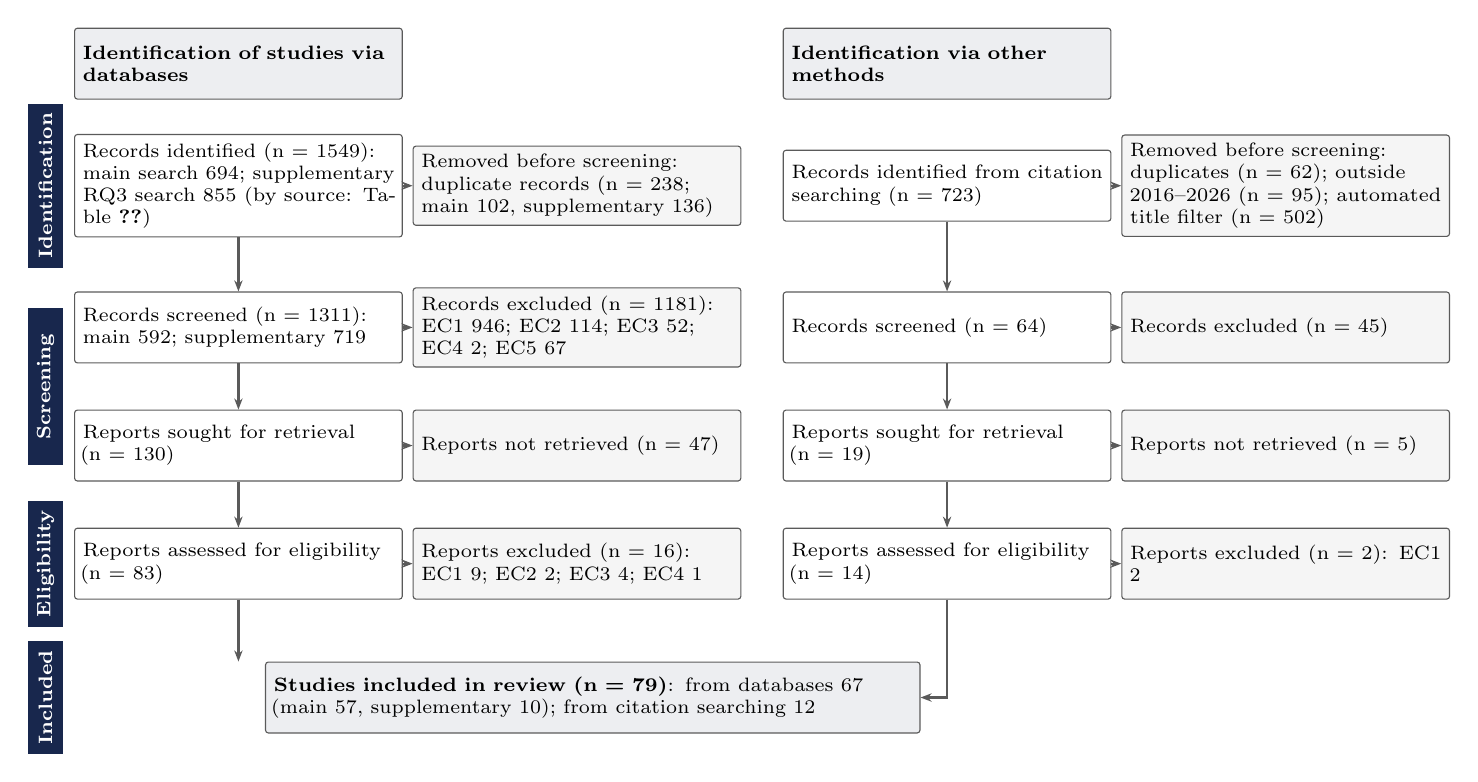
\begin{tikzpicture}[font=\scriptsize, box/.style={draw=boxline, rounded corners=1pt, align=left, text width=3.95cm, inner sep=3pt, minimum height=0.9cm}, ex/.style={box, fill=rowgray}, arr/.style={-{Stealth[length=4pt]}, thick, boxline}, stage/.style={fill=navy, text=white, font=\scriptsize\bfseries, rotate=90, minimum width=2.0cm, minimum height=0.45cm, align=center}]
\node[box, fill=navy!8] (h1) at (0.9,0.95) {\textbf{Identification of studies via databases}};
\node[box, fill=navy!8] (h2) at (9.9,0.95) {\textbf{Identification via other methods}};
\node[box] (a1) at (0.9,-0.6) {Records identified (n~=~\dbAllId):\\ main search \idTotal; supplementary RQ3 search \spTotal{} (by source: Table~\ref{tab:sources})};
\node[ex] (b1) at (5.2,-0.6) {Removed before screening:\\ duplicate records (n~=~\dbAllDup; main \dupRemoved, supplementary \spDupRemoved)};
\node[box] (c1) at (9.9,-0.6) {Records identified from citation searching (n~=~\csHarvested)};
\node[ex] (d1) at (14.2,-0.6) {Removed before screening:\\ duplicates (n~=~\csDupAll); outside 2016--2026 (n~=~\csYear); automated title filter (n~=~\csTitleFilter)};
\node[box] (a2) at (0.9,-2.4) {Records screened (n~=~\dbAllScreened):\\ main \taScreened; supplementary \spScreened};
\node[ex] (b2) at (5.2,-2.4) {Records excluded (n~=~\dbAllExcluded): EC1 \dbAllExOne; EC2 \dbAllExTwo; EC3 \dbAllExThree; EC4 \dbAllExFour; EC5 \dbAllExFive};
\node[box] (c2) at (9.9,-2.4) {Records screened (n~=~\csScreened)};
\node[ex] (d2) at (14.2,-2.4) {Records excluded (n~=~\csTaExcluded)};
\node[box] (a3) at (0.9,-3.9) {Reports sought for retrieval (n~=~\dbAllSought)};
\node[ex] (b3) at (5.2,-3.9) {Reports not retrieved (n~=~\dbAllNotRetrieved)};
\node[box] (c3) at (9.9,-3.9) {Reports sought for retrieval (n~=~\csSought)};
\node[ex] (d3) at (14.2,-3.9) {Reports not retrieved (n~=~\csNotRetrieved)};
\node[box] (a4) at (0.9,-5.4) {Reports assessed for eligibility (n~=~\dbAllAssessed)};
\node[ex] (b4) at (5.2,-5.4) {Reports excluded (n~=~\dbAllFtExcluded): EC1 \dbAllFtExOne; EC2 \dbAllFtExTwo; EC3 \dbAllFtExThree; EC4 \dbAllFtExFour};
\node[box] (c4) at (9.9,-5.4) {Reports assessed for eligibility (n~=~\csAssessed)};
\node[ex] (d4) at (14.2,-5.4) {Reports excluded (n~=~\csFtExcluded): EC1 \csFtExcluded};
\node[box, fill=navy!8, text width=8.1cm] (inc) at (5.4,-7.1) {\textbf{Studies included in review (n~=~\totalIncluded)}: from databases \dbAllIncluded{} (main \dbIncluded, supplementary \spIncluded); from citation searching \csIncluded};
\foreach \u/\v in {a1/b1,a2/b2,a3/b3,a4/b4,c1/d1,c2/d2,c3/d3,c4/d4} \draw[arr] (\u) -- (\v);
\foreach \u/\v in {a1/a2,a2/a3,a3/a4,c1/c2,c2/c3,c3/c4} \draw[arr] (\u) -- (\v);
\draw[arr] (a4.south) -- (a4.south |- inc.north);
\draw[arr] (c4.south) |- (inc.east);
\node[stage] at (-1.55,-0.6) {Identification};
\node[stage] at (-1.55,-3.15) {Screening};
\node[stage, minimum width=1.2cm] at (-1.55,-5.4) {Eligibility};
\node[stage, minimum width=1.2cm] at (-1.55,-7.1) {Included};
\end{tikzpicture}}
\caption{PRISMA 2020 flow diagram \cite{page2021}. Counts are generated from the screening workbook (sheet \texttt{PRISMA\_Counts}), and every arithmetic step is checked by formula.}\label{fig:prisma}
\end{figure}

\section{Data extraction and quality appraisal}
For each included study we extracted the Study ID, full citation, publication details and verified peer-review status (Crossref, the arXiv record, the PDF itself or Semantic Scholar), problem, RQs informed, method, datasets, evaluation, findings, limitations, reproducibility, quality scores with notes, and the decision evidence. Items a paper does not report are marked ``Not reported'' (Appendix~C; workbook sheets \texttt{Extraction}, \texttt{Quality}). Quality was appraised with ten items scored Yes = 1, Partial = 0.5, No = 0 or N/A: Q1 clear aims; Q2 replicable method; Q3 datasets described; Q4 appropriate comparison; Q5 well-defined stability measure; Q6 evidence sufficient (scale, repetitions, statistics); Q7 limitations discussed; Q8 code or data available; Q9 ethics, privacy or regulation addressed where relevant; Q10 randomness controlled and reported. The score is the share of applicable items; we rate 80\% or above as high, 60--79\% as moderate and below 60\% as low. Scores weight the synthesis but did not exclude any study; a note explains every score below 1. The mean score was \qaMean\%: \qaHigh{} studies were high, \qaMod{} moderate and \qaLow{} low \cite{S15,S55}. The weakest items were code or data availability (Q8, mean 0.59), ethics where applicable (Q9, 0.60 over 25 studies) and limitations (Q7, 0.70). The included set meets the recency targets: \incSinceTwentyTwo{} of \totalIncluded{} studies are from 2022 or later and \incSinceTwentyFive{} from 2025 or later. It also contains \incBeforeTwentyTwo{} studies from before 2022, among them foundational work on explainer stability \cite{S01,S04,S08}, and \mapreview{} reviews \evreview. By type, there are \incJournal{} journal articles, \incConference{} conference papers, \incWorkshop{} workshop papers and \incPreprint{} preprints; the preprints are labelled as not peer reviewed. The set exceeds the minimum target because the topic is very active and RQ3 added a supplementary search. By question, \rqOne{} studies inform RQ1, \rqTwo{} RQ2 and \rqThree{} RQ3.

\section{Thematic synthesis and research gap}\label{sec:synth}
% SYNTHESIS-START
\textbf{Theme 1: measurement is fragmented (RQ1).} Studies use at least five families of stability measure: top-$k$ overlap \cite{S07,S08,S21,S36,S54}, rank agreement (Spearman, Kendall, sequential) \cite{S29,S34,S53,S56}, dispersion of attribution values \cite{S24,S38,S47}, LIME-specific indices \cite{S10,S39} and Lipschitz-type ratios \cite{S01,S05,S09,S23,S25}. Regimes vary as much: \mapsrcretrain{} vary the model, \mapsrcnoise{} only the explainer's sampling, \mapsrcperturb{} perturb inputs and \mapsrcadversarial{} use attacks. Only \mapst{} apply inferential statistics, and only \mapnoiseandperturb{} measure run-to-run explainer noise alongside perturbation effects \evnoiseandperturb, none using it as a floor.

\textbf{Theme 2: stable predictions do not guarantee stable explanations (RQ2).} The \mappe{} studies relating prediction-side quantities to explanation change agree the link is weak. Under attack, prediction robustness and explanation stability were distinct axes \cite{S59}; quantised models kept their ROC-AUC while SHAP rankings changed \cite{S50}; prediction-equivalent models from different hypothesis classes gave different attributions \cite{S75}; and better accuracy did not bring more reliable explanations \cite{S51,S79}. Only \mappp{} studies keep perturbations that leave the prediction unchanged \evpp, and none in our extraction tests at the instance level whether the size of the prediction change predicts that of the explanation change.

\textbf{Theme 3: instability has identifiable mechanisms (RQ3).} Instability is tied to a threshold or boundary in \mapmechthr{} studies \evmechthr. Crossing a split in a single tree makes the Lipschitz ratio of random-forest SHAP diverge, which combining weak-learner explanations reduces \cite{S25}. XGBoost's piecewise-constant surface defeats gradient-free attacks yet leaves explanations unstable \cite{S59}; gradient-boosted trees show the same instability near segment boundaries as smooth non-linear models \cite{S77}. Explainer uncertainty grows with decision-boundary complexity \cite{S19} and falls with predictor smoothness \cite{S23}. For LIME, the random neighbourhood with its sample-size and proximity settings drives repeated-call variation \cite{S02,S08,S10}. Collinearity is the best-documented data mechanism (\mapmechcoll{} studies) \evmechcoll: 68\% of 77 datasets showed SHAP instability, with rankings of correlated pairs close to a coin flip \cite{S43}. KernelSHAP adds Monte-Carlo error \cite{S18,S21,S31}, whereas TreeSHAP was near-deterministic \cite{S45,S46}. No study, however, counts how many split thresholds or bin edges a perturbation crosses.

\textbf{Theme 4: predicting instability is possible but rarely cheap (RQ3).} \mapdiag{} studies attach an uncertainty or reliability estimate, for example Bayesian or bootstrap intervals \cite{S05,S11,S35}, distributional SHAP \cite{S73,S74}, model-set importance clouds \cite{S71} and tree-ensemble epistemic uncertainty \cite{S47}. Most need resampling or repeated calls, the cost a warning score should avoid. Only \mapdiagfree{} validate a perturbation-free predictor against observed instability: epistemic uncertainty correlated strongly and negatively with stability \cite{S52}, instability was lower where forecast uncertainty was low \cite{S77}, and a reliability score built from feature-interaction density and axis-aligned tree splits tracked disagreement between prediction-equivalent models \cite{S75}, which is related to but distinct from perturbation stability.

\textbf{Strength of evidence.} \incPreprint{} included studies are preprints, \incWorkshop{} workshop papers. Themes 1--3 also rest on peer-reviewed studies, but all three cheap predictors in Theme 4 are preprints, so that evidence is weak. Domains concentrate on credit, fraud, intrusion detection and health.

\textbf{Evidence-based gap.} No included study (i) combines an instance-level prediction-preserving filter with both SHAP and LIME, linear and tree-ensemble classifiers and a statistical test; the closest, Tolay \cite{S62}, uses TreeSHAP only and is a preprint. No study (ii) counts split-threshold or bin-edge crossings as the cause of a change, or (iii) builds a fragility score from the trained trees alone and validates it against observed instability with a discrimination measure such as AUROC.

\textbf{How this changes the Assignment 1 problem.} The problem stays; its framing is sharpened. Novelty must be narrowed: prediction-preserving filters exist \cite{S09,S25,S62}; what is new is testing the prediction-to-explanation link for SHAP and LIME together on linear and tree-ensemble models against each explainer's noise floor. It should explain instability, not only measure it, by logging threshold and bin-edge crossings and controlling collinearity and class imbalance \cite{S29,S43,S53}. Finally, it should test whether a score computed from the trees alone can flag fragile explanations before any perturbation, with uncertainty-based scores \cite{S52,S77} as comparison. The revised statement reads: \textit{under prediction-preserving perturbations, does the size of a prediction change indicate the size of the SHAP or LIME explanation change for logistic regression, random forest and XGBoost beyond each explainer's own noise; is the change explained by split-threshold and bin-edge crossings; and can a score computed from the model alone predict it?}
% SYNTHESIS-END

\section{Limitations}\label{sec:lim}
(1) ACM Digital Library, Scopus and Web of Science were not searched, and OpenAlex was used only for piloting; Semantic Scholar and DBLP cover much of the same literature, but gaps remain. (2) Phrase-based terms missed five of the \nKnown{} benchmark papers \cite{hwang2025,decker2025,lin2023,takefuji2025,hasnain2026}, four of them cited in Assignment 1. They were not added, because the documented search did not retrieve them; they are flagged for the next search update. Takefuji and Hasnain et al.\ remain relevant context for RQ2. (3) \totalNotRetrieved{} of \totalSought{} reports (\the\numexpr(\totalNotRetrieved*100+\totalSought/2)/\totalSought\relax\%) could not be retrieved, \spNotRetrieved{} of them from the supplementary search, mostly paywalled IEEE conference papers and open-access papers behind bot checks. The list (workbook sheet \texttt{FullText}; \texttt{links/reports\_not\_retrieved.csv}) can be completed through the HEC Digital Library. (4) Dual screening and the kappa statistic are pending. (5) Citation searching used an automated title filter before manual screening, which may have dropped relevant titles that use other wording. (6) Many included studies (\incSinceTwentyFive{}) are from 2025--2026 and \incPreprint{} are preprints, so their findings may change. (7) The supplementary RQ3 search omitted ScienceDirect, and papers that discuss thresholds or uncertainty only in the full text may have been missed.

\section{Contribution statement and AI-use disclosure}\label{sec:contrib}
\textit{Proposed division, to be confirmed or edited by the team before submission.} \textbf{Shahoud Shahid:} leads RQ1; owns the IEEE Xplore, ScienceDirect and DBLP searches; confirms the title-abstract decisions; verifies extraction and quality scores for S01--S35. \textbf{Saif Shahzad:} leads RQ2; owns the arXiv and Semantic Scholar searches and citation searching; performs the independent dual screening; verifies S36--S79. \textbf{Both:} RQ3 (mechanisms and fragility predictors) and its supplementary search, the synthesis and the final edit. \textbf{AI use:} with the team's direction, an AI assistant (Claude, Anthropic) ran the documented searches through public APIs and web interfaces, de-duplicated records, drafted the screening and full-text decisions with page or section evidence, extracted data, scored quality and drafted this report. No source, result or count was invented: every figure is generated from the logged data files in the accompanying workbook and scripts. The team should verify the decisions and disclose this assistance as course policy requires.

{\small
\bibliographystyle{IEEEtran}
\bibliography{included_studies,refs_methods}
}

\clearpage
\appendix
\counterwithin{table}{section}
\renewcommand{\thetable}{\Alph{section}.\arabic{table}}
\section{Search log and refinement log}
{\footnotesize\setlength{\tabcolsep}{2pt}\begin{longtable}{@{}P{0.4cm}P{2.2cm}P{8.0cm}P{2.5cm}P{1.0cm}P{1.1cm}@{}}
\caption{Search log (main searches 24 October 2026; supplementary RQ3 searches 24--25 October 2026). Exact strings as submitted.}\label{tab:searchlog}\\
\toprule \# & Source & Exact search string & Fields; filters & Results & Exported \\ \midrule \endfirsthead
\toprule \# & Source & Exact search string & Fields; filters & Results & Exported \\ \midrule \endhead
\bottomrule \endfoot
1 & IEEE Xplore (REST search, web interface) & {\ttfamily\scriptsize (\textquotedbl{}All Metadata\textquotedbl{}:SHAP OR\allowbreak{} \textquotedbl{}All Metadata\textquotedbl{}:\textquotedbl{}Shapley additive\textquotedbl{} OR\allowbreak{} \textquotedbl{}All Metadata\textquotedbl{}:\textquotedbl{}Shapley values\textquotedbl{} OR\allowbreak{} \textquotedbl{}All Metadata\textquotedbl{}:TreeSHAP OR\allowbreak{} \textquotedbl{}All Metadata\textquotedbl{}:KernelSHAP OR\allowbreak{} \textquotedbl{}All Metadata\textquotedbl{}:LIME OR\allowbreak{} \textquotedbl{}All Metadata\textquotedbl{}:\textquotedbl{}local interpretable model-agnostic\textquotedbl{} OR\allowbreak{} \textquotedbl{}All Metadata\textquotedbl{}:\textquotedbl{}feature attribution*\textquotedbl{} OR\allowbreak{} \textquotedbl{}All Metadata\textquotedbl{}:\textquotedbl{}post-hoc explanation*\textquotedbl{} OR\allowbreak{} \textquotedbl{}All Metadata\textquotedbl{}:\textquotedbl{}local explanation*\textquotedbl{}) AND\allowbreak{} (\textquotedbl{}All Metadata\textquotedbl{}:\textquotedbl{}explanation stability\textquotedbl{} OR\allowbreak{} \textquotedbl{}All Metadata\textquotedbl{}:\textquotedbl{}stability of explanations\textquotedbl{} OR\allowbreak{} \textquotedbl{}All Metadata\textquotedbl{}:\textquotedbl{}stability of model explanations\textquotedbl{} OR\allowbreak{} \textquotedbl{}All Metadata\textquotedbl{}:\textquotedbl{}stability of LIME\textquotedbl{} OR\allowbreak{} \textquotedbl{}All Metadata\textquotedbl{}:\textquotedbl{}LIME stability\textquotedbl{} OR\allowbreak{} \textquotedbl{}All Metadata\textquotedbl{}:\textquotedbl{}stability of SHAP\textquotedbl{} OR\allowbreak{} \textquotedbl{}All Metadata\textquotedbl{}:\textquotedbl{}SHAP stability\textquotedbl{} OR\allowbreak{} \textquotedbl{}All Metadata\textquotedbl{}:\textquotedbl{}attribution stability\textquotedbl{} OR\allowbreak{} \textquotedbl{}All Metadata\textquotedbl{}:\textquotedbl{}explanation instability\textquotedbl{} OR\allowbreak{} \textquotedbl{}All Metadata\textquotedbl{}:\textquotedbl{}unstable explanations\textquotedbl{} OR\allowbreak{} \textquotedbl{}All Metadata\textquotedbl{}:\textquotedbl{}stable explanations\textquotedbl{} OR\allowbreak{} \textquotedbl{}All Metadata\textquotedbl{}:\textquotedbl{}explanation robustness\textquotedbl{} OR\allowbreak{} \textquotedbl{}All Metadata\textquotedbl{}:\textquotedbl{}robustness of explanations\textquotedbl{} OR\allowbreak{} \textquotedbl{}All Metadata\textquotedbl{}:\textquotedbl{}robust explanations\textquotedbl{} OR\allowbreak{} \textquotedbl{}All Metadata\textquotedbl{}:\textquotedbl{}robustness of interpretability\textquotedbl{} OR\allowbreak{} \textquotedbl{}All Metadata\textquotedbl{}:\textquotedbl{}attribution robustness\textquotedbl{} OR\allowbreak{} \textquotedbl{}All Metadata\textquotedbl{}:\textquotedbl{}explanation consistency\textquotedbl{} OR\allowbreak{} \textquotedbl{}All Metadata\textquotedbl{}:\textquotedbl{}explanation fragility\textquotedbl{} OR\allowbreak{} \textquotedbl{}All Metadata\textquotedbl{}:\textquotedbl{}stability indices\textquotedbl{}) AND\allowbreak{} (\textquotedbl{}All Metadata\textquotedbl{}:tabular OR\allowbreak{} \textquotedbl{}All Metadata\textquotedbl{}:\textquotedbl{}structured data\textquotedbl{} OR\allowbreak{} \textquotedbl{}All Metadata\textquotedbl{}:\textquotedbl{}tree ensemble*\textquotedbl{} OR\allowbreak{} \textquotedbl{}All Metadata\textquotedbl{}:\textquotedbl{}tree-based\textquotedbl{} OR\allowbreak{} \textquotedbl{}All Metadata\textquotedbl{}:\textquotedbl{}random forest*\textquotedbl{} OR\allowbreak{} \textquotedbl{}All Metadata\textquotedbl{}:XGBoost OR\allowbreak{} \textquotedbl{}All Metadata\textquotedbl{}:\textquotedbl{}gradient boosting\textquotedbl{} OR\allowbreak{} \textquotedbl{}All Metadata\textquotedbl{}:LightGBM OR\allowbreak{} \textquotedbl{}All Metadata\textquotedbl{}:\textquotedbl{}logistic regression\textquotedbl{} OR\allowbreak{} \textquotedbl{}All Metadata\textquotedbl{}:\textquotedbl{}credit scoring\textquotedbl{} OR\allowbreak{} \textquotedbl{}All Metadata\textquotedbl{}:\textquotedbl{}credit risk\textquotedbl{} OR\allowbreak{} \textquotedbl{}All Metadata\textquotedbl{}:fraud)} & All Metadata; Publication year 2016-2026 & 48 & 48 \\
\multicolumn{6}{@{}p{15.9cm}@{}}{\scriptsize\textit{Note:} Final string after piloting (see Refinement\_\allowbreak{}Log). Trailing * used for truncation.} \\[2pt]
2 & ScienceDirect (web search) SD1 & {\ttfamily\scriptsize Find articles with these terms: (SHAP OR\allowbreak{} \textquotedbl{}Shapley additive\textquotedbl{} OR\allowbreak{} \textquotedbl{}Shapley values\textquotedbl{} OR\allowbreak{} LIME OR\allowbreak{} \textquotedbl{}local interpretable model-agnostic\textquotedbl{} OR\allowbreak{} \textquotedbl{}feature attribution\textquotedbl{} OR\allowbreak{} \textquotedbl{}post-hoc explanation\textquotedbl{} OR\allowbreak{} \textquotedbl{}local explanation\textquotedbl{} OR\allowbreak{} \textquotedbl{}post hoc explanation\textquotedbl{})  \textbar{}\allowbreak{}  Title, abstract or author-specified keywords: (\{explanation stability\} OR\allowbreak{} \{stability of explanations\} OR\allowbreak{} \{stability of model explanations\} OR\allowbreak{} \{stability of LIME\} OR\allowbreak{} \{LIME stability\} OR\allowbreak{} \{stability of SHAP\} OR\allowbreak{} \{SHAP stability\})} & qs: full record; tak: title-abstract-keywords; Years 2016-2026 & 59 & 59 \\
\multicolumn{6}{@{}p{15.9cm}@{}}{\scriptsize\textit{Note:} Braces force exact phrases. ScienceDirect allows at most 8 Boolean connectors per field, so the stability concept was split across SD1-SD3.} \\[2pt]
3 & ScienceDirect (web search) SD2 & {\ttfamily\scriptsize Find articles with these terms: (SHAP OR\allowbreak{} \textquotedbl{}Shapley additive\textquotedbl{} OR\allowbreak{} \textquotedbl{}Shapley values\textquotedbl{} OR\allowbreak{} LIME OR\allowbreak{} \textquotedbl{}local interpretable model-agnostic\textquotedbl{} OR\allowbreak{} \textquotedbl{}feature attribution\textquotedbl{} OR\allowbreak{} \textquotedbl{}post-hoc explanation\textquotedbl{} OR\allowbreak{} \textquotedbl{}local explanation\textquotedbl{} OR\allowbreak{} \textquotedbl{}post hoc explanation\textquotedbl{})  \textbar{}\allowbreak{}  Title, abstract or author-specified keywords: (\{attribution stability\} OR\allowbreak{} \{explanation instability\} OR\allowbreak{} \{unstable explanations\} OR\allowbreak{} \{stable explanations\} OR\allowbreak{} \{explanation robustness\} OR\allowbreak{} \{robustness of explanations\})} & qs: full record; tak: title-abstract-keywords; Years 2016-2026 & 37 & 37 \\
\multicolumn{6}{@{}p{15.9cm}@{}}{\scriptsize\textit{Note:} Second part of the stability concept.} \\[2pt]
4 & ScienceDirect (web search) SD3 & {\ttfamily\scriptsize Find articles with these terms: (SHAP OR\allowbreak{} \textquotedbl{}Shapley additive\textquotedbl{} OR\allowbreak{} \textquotedbl{}Shapley values\textquotedbl{} OR\allowbreak{} LIME OR\allowbreak{} \textquotedbl{}local interpretable model-agnostic\textquotedbl{} OR\allowbreak{} \textquotedbl{}feature attribution\textquotedbl{} OR\allowbreak{} \textquotedbl{}post-hoc explanation\textquotedbl{} OR\allowbreak{} \textquotedbl{}local explanation\textquotedbl{} OR\allowbreak{} \textquotedbl{}post hoc explanation\textquotedbl{})  \textbar{}\allowbreak{}  Title, abstract or author-specified keywords: (\{robust explanations\} OR\allowbreak{} \{robustness of interpretability\} OR\allowbreak{} \{attribution robustness\} OR\allowbreak{} \{explanation consistency\} OR\allowbreak{} \{explanation fragility\} OR\allowbreak{} \{stability indices\})} & qs: full record; tak: title-abstract-keywords; Years 2016-2026 & 0 & 0 \\
\multicolumn{6}{@{}p{15.9cm}@{}}{\scriptsize\textit{Note:} Third part of the stability concept; no records.} \\[2pt]
5 & arXiv (export API) & {\ttfamily\scriptsize (abs:SHAP OR\allowbreak{} abs:\textquotedbl{}Shapley additive\textquotedbl{} OR\allowbreak{} abs:\textquotedbl{}Shapley values\textquotedbl{} OR\allowbreak{} abs:TreeSHAP OR\allowbreak{} abs:KernelSHAP OR\allowbreak{} abs:LIME OR\allowbreak{} abs:\textquotedbl{}local interpretable model-agnostic\textquotedbl{} OR\allowbreak{} abs:\textquotedbl{}feature attribution\textquotedbl{} OR\allowbreak{} abs:\textquotedbl{}post-hoc explanation\textquotedbl{} OR\allowbreak{} abs:\textquotedbl{}local explanation\textquotedbl{}) AND\allowbreak{} (abs:\textquotedbl{}explanation stability\textquotedbl{} OR\allowbreak{} abs:\textquotedbl{}stability of explanations\textquotedbl{} OR\allowbreak{} abs:\textquotedbl{}stability of model explanations\textquotedbl{} OR\allowbreak{} abs:\textquotedbl{}stability of LIME\textquotedbl{} OR\allowbreak{} abs:\textquotedbl{}LIME stability\textquotedbl{} OR\allowbreak{} abs:\textquotedbl{}stability of SHAP\textquotedbl{} OR\allowbreak{} abs:\textquotedbl{}SHAP stability\textquotedbl{} OR\allowbreak{} abs:\textquotedbl{}attribution stability\textquotedbl{} OR\allowbreak{} abs:\textquotedbl{}explanation instability\textquotedbl{} OR\allowbreak{} abs:\textquotedbl{}unstable explanations\textquotedbl{} OR\allowbreak{} abs:\textquotedbl{}stable explanations\textquotedbl{} OR\allowbreak{} abs:\textquotedbl{}explanation robustness\textquotedbl{} OR\allowbreak{} abs:\textquotedbl{}robustness of explanations\textquotedbl{} OR\allowbreak{} abs:\textquotedbl{}robust explanations\textquotedbl{} OR\allowbreak{} abs:\textquotedbl{}robustness of interpretability\textquotedbl{} OR\allowbreak{} abs:\textquotedbl{}attribution robustness\textquotedbl{} OR\allowbreak{} abs:\textquotedbl{}explanation consistency\textquotedbl{} OR\allowbreak{} abs:\textquotedbl{}explanation fragility\textquotedbl{} OR\allowbreak{} abs:\textquotedbl{}stability indices\textquotedbl{}) AND\allowbreak{} (abs:tabular OR\allowbreak{} abs:\textquotedbl{}structured data\textquotedbl{} OR\allowbreak{} abs:\textquotedbl{}tree ensemble\textquotedbl{} OR\allowbreak{} abs:\textquotedbl{}tree-based\textquotedbl{} OR\allowbreak{} abs:\textquotedbl{}random forest\textquotedbl{} OR\allowbreak{} abs:XGBoost OR\allowbreak{} abs:\textquotedbl{}gradient boosting\textquotedbl{} OR\allowbreak{} abs:LightGBM OR\allowbreak{} abs:\textquotedbl{}logistic regression\textquotedbl{} OR\allowbreak{} abs:\textquotedbl{}credit scoring\textquotedbl{} OR\allowbreak{} abs:\textquotedbl{}credit risk\textquotedbl{} OR\allowbreak{} abs:fraud) AND\allowbreak{} submittedDate:[201601010000 TO 202612312359]} & abs (abstract); submittedDate 2016-01-01 to 2026-12-31 & 29 & 29 \\
\multicolumn{6}{@{}p{15.9cm}@{}}{\scriptsize\textit{Note:} arXiv does not support truncation, so * was removed.} \\[2pt]
6 & Semantic Scholar (Graph API, bulk search) & {\ttfamily\scriptsize (SHAP \textbar{}\allowbreak{} \textquotedbl{}Shapley additive\textquotedbl{} \textbar{}\allowbreak{} \textquotedbl{}Shapley values\textquotedbl{} \textbar{}\allowbreak{} TreeSHAP \textbar{}\allowbreak{} KernelSHAP \textbar{}\allowbreak{} LIME \textbar{}\allowbreak{} \textquotedbl{}local interpretable model-agnostic\textquotedbl{} \textbar{}\allowbreak{} \textquotedbl{}feature attribution\textquotedbl{} \textbar{}\allowbreak{} \textquotedbl{}post-hoc explanation\textquotedbl{} \textbar{}\allowbreak{} \textquotedbl{}local explanation\textquotedbl{}) + (\textquotedbl{}explanation stability\textquotedbl{} \textbar{}\allowbreak{} \textquotedbl{}stability of explanations\textquotedbl{} \textbar{}\allowbreak{} \textquotedbl{}stability of model explanations\textquotedbl{} \textbar{}\allowbreak{} \textquotedbl{}stability of LIME\textquotedbl{} \textbar{}\allowbreak{} \textquotedbl{}LIME stability\textquotedbl{} \textbar{}\allowbreak{} \textquotedbl{}stability of SHAP\textquotedbl{} \textbar{}\allowbreak{} \textquotedbl{}SHAP stability\textquotedbl{} \textbar{}\allowbreak{} \textquotedbl{}attribution stability\textquotedbl{} \textbar{}\allowbreak{} \textquotedbl{}explanation instability\textquotedbl{} \textbar{}\allowbreak{} \textquotedbl{}unstable explanations\textquotedbl{} \textbar{}\allowbreak{} \textquotedbl{}stable explanations\textquotedbl{} \textbar{}\allowbreak{} \textquotedbl{}explanation robustness\textquotedbl{} \textbar{}\allowbreak{} \textquotedbl{}robustness of explanations\textquotedbl{} \textbar{}\allowbreak{} \textquotedbl{}robust explanations\textquotedbl{} \textbar{}\allowbreak{} \textquotedbl{}robustness of interpretability\textquotedbl{} \textbar{}\allowbreak{} \textquotedbl{}attribution robustness\textquotedbl{} \textbar{}\allowbreak{} \textquotedbl{}explanation consistency\textquotedbl{} \textbar{}\allowbreak{} \textquotedbl{}explanation fragility\textquotedbl{} \textbar{}\allowbreak{} \textquotedbl{}stability indices\textquotedbl{}) + (tabular \textbar{}\allowbreak{} \textquotedbl{}structured data\textquotedbl{} \textbar{}\allowbreak{} \textquotedbl{}tree ensemble\textquotedbl{} \textbar{}\allowbreak{} \textquotedbl{}tree-based\textquotedbl{} \textbar{}\allowbreak{} \textquotedbl{}random forest\textquotedbl{} \textbar{}\allowbreak{} XGBoost \textbar{}\allowbreak{} \textquotedbl{}gradient boosting\textquotedbl{} \textbar{}\allowbreak{} LightGBM \textbar{}\allowbreak{} \textquotedbl{}logistic regression\textquotedbl{} \textbar{}\allowbreak{} \textquotedbl{}credit scoring\textquotedbl{} \textbar{}\allowbreak{} \textquotedbl{}credit risk\textquotedbl{} \textbar{}\allowbreak{} fraud)} & Title and abstract (API default); year 2016-2026 & 364 & 364 \\
\multicolumn{6}{@{}p{15.9cm}@{}}{\scriptsize\textit{Note:} Multidisciplinary source used in place of OpenAlex after the OpenAlex daily API budget ran out during piloting. \textbar{} = OR, + = AND.} \\[2pt]
7 & DBLP (web search) & {\ttfamily\scriptsize stability\$\textbar{}\allowbreak{}stable\$\textbar{}\allowbreak{}unstable\$\textbar{}\allowbreak{}instability\$\textbar{}\allowbreak{}stabilized\$\textbar{}\allowbreak{}stabilizing\$\textbar{}\allowbreak{}stabilised\$\textbar{}\allowbreak{}fragility\$\textbar{}\allowbreak{}fragile\$ shap\$\textbar{}\allowbreak{}lime\$\textbar{}\allowbreak{}shapley\$\textbar{}\allowbreak{}explanation\$\textbar{}\allowbreak{}explanations\$\textbar{}\allowbreak{}attribution\$\textbar{}\allowbreak{}attributions\$} & Title (DBLP indexes titles only); Year 2016-2026 applied after export & 174 & 157 \\
\multicolumn{6}{@{}p{15.9cm}@{}}{\scriptsize\textit{Note:} \$ = exact word, \textbar{} = OR, space = AND. 17 records before 2016 removed.} \\[2pt]
8 & Citation searching (Semantic Scholar citation graph) & {\ttfamily\scriptsize Backward (references) and forward (citations) of 7 seed studies: Ballegeer 2025, Agarwal 2022, Visani 2022, Zhou 2021, Tzionis 2026, Rajhans 2026, Pala 2024} & Reference and citation lists; Year 2016-2026; title must contain a stability term AND an explanation term; not already identified & 723 & 70 \\
\multicolumn{6}{@{}p{15.9cm}@{}}{\scriptsize\textit{Note:} Reported in the PRISMA \textquotedbl{}other methods\textquotedbl{} column.} \\[2pt]
9 & ACM Digital Library & {\ttfamily\scriptsize Prepared (see acm\_\allowbreak{}q.txt in search\_\allowbreak{}scripts) but not executed} & Title, Abstract, Keyword; - & Not run & 0 \\
\multicolumn{6}{@{}p{15.9cm}@{}}{\scriptsize\textit{Note:} The site showed a Cloudflare bot check; it was not bypassed. ACM conference papers are partly covered through DBLP and Semantic Scholar.} \\[2pt]
10 & SpringerLink & {\ttfamily\scriptsize Prepared (see springer\_\allowbreak{}q.txt) but not used} & -; - & Not run & 0 \\
\multicolumn{6}{@{}p{15.9cm}@{}}{\scriptsize\textit{Note:} No title/\allowbreak{}abstract field restriction (searches full text), so results could not be made comparable.} \\[2pt]
11 & IEEE Xplore - supplementary (RQ3) & {\ttfamily\scriptsize (\textquotedbl{}All Metadata\textquotedbl{}:SHAP OR\allowbreak{} \textquotedbl{}All Metadata\textquotedbl{}:\textquotedbl{}Shapley additive\textquotedbl{} OR\allowbreak{} \textquotedbl{}All Metadata\textquotedbl{}:\textquotedbl{}Shapley values\textquotedbl{} OR\allowbreak{} \textquotedbl{}All Metadata\textquotedbl{}:TreeSHAP OR\allowbreak{} \textquotedbl{}All Metadata\textquotedbl{}:KernelSHAP OR\allowbreak{} \textquotedbl{}All Metadata\textquotedbl{}:LIME OR\allowbreak{} \textquotedbl{}All Metadata\textquotedbl{}:\textquotedbl{}local interpretable model-agnostic\textquotedbl{} OR\allowbreak{} \textquotedbl{}All Metadata\textquotedbl{}:\textquotedbl{}feature attribution*\textquotedbl{} OR\allowbreak{} \textquotedbl{}All Metadata\textquotedbl{}:\textquotedbl{}post-hoc explanation*\textquotedbl{} OR\allowbreak{} \textquotedbl{}All Metadata\textquotedbl{}:\textquotedbl{}local explanation*\textquotedbl{}) AND\allowbreak{} (\textquotedbl{}All Metadata\textquotedbl{}:stability OR\allowbreak{} \textquotedbl{}All Metadata\textquotedbl{}:stable OR\allowbreak{} \textquotedbl{}All Metadata\textquotedbl{}:unstable OR\allowbreak{} \textquotedbl{}All Metadata\textquotedbl{}:instability OR\allowbreak{} \textquotedbl{}All Metadata\textquotedbl{}:robustness OR\allowbreak{} \textquotedbl{}All Metadata\textquotedbl{}:robust OR\allowbreak{} \textquotedbl{}All Metadata\textquotedbl{}:fragility OR\allowbreak{} \textquotedbl{}All Metadata\textquotedbl{}:fragile OR\allowbreak{} \textquotedbl{}All Metadata\textquotedbl{}:consistency OR\allowbreak{} \textquotedbl{}All Metadata\textquotedbl{}:uncertainty) AND\allowbreak{} (\textquotedbl{}All Metadata\textquotedbl{}:\textquotedbl{}split threshold*\textquotedbl{} OR\allowbreak{} \textquotedbl{}All Metadata\textquotedbl{}:\textquotedbl{}split point*\textquotedbl{} OR\allowbreak{} \textquotedbl{}All Metadata\textquotedbl{}:\textquotedbl{}decision threshold*\textquotedbl{} OR\allowbreak{} \textquotedbl{}All Metadata\textquotedbl{}:\textquotedbl{}decision boundar*\textquotedbl{} OR\allowbreak{} \textquotedbl{}All Metadata\textquotedbl{}:discretiz* OR\allowbreak{} \textquotedbl{}All Metadata\textquotedbl{}:discretis* OR\allowbreak{} \textquotedbl{}All Metadata\textquotedbl{}:\textquotedbl{}bin edge*\textquotedbl{} OR\allowbreak{} \textquotedbl{}All Metadata\textquotedbl{}:binning OR\allowbreak{} \textquotedbl{}All Metadata\textquotedbl{}:\textquotedbl{}piecewise constant\textquotedbl{} OR\allowbreak{} \textquotedbl{}All Metadata\textquotedbl{}:\textquotedbl{}tree structure\textquotedbl{} OR\allowbreak{} \textquotedbl{}All Metadata\textquotedbl{}:\textquotedbl{}decision path*\textquotedbl{} OR\allowbreak{} \textquotedbl{}All Metadata\textquotedbl{}:\textquotedbl{}fragility score\textquotedbl{} OR\allowbreak{} \textquotedbl{}All Metadata\textquotedbl{}:\textquotedbl{}instability score\textquotedbl{} OR\allowbreak{} \textquotedbl{}All Metadata\textquotedbl{}:\textquotedbl{}stability score\textquotedbl{} OR\allowbreak{} \textquotedbl{}All Metadata\textquotedbl{}:\textquotedbl{}reliability score\textquotedbl{} OR\allowbreak{} \textquotedbl{}All Metadata\textquotedbl{}:\textquotedbl{}uncertainty estimat*\textquotedbl{} OR\allowbreak{} \textquotedbl{}All Metadata\textquotedbl{}:\textquotedbl{}uncertainty quantification\textquotedbl{} OR\allowbreak{} \textquotedbl{}All Metadata\textquotedbl{}:\textquotedbl{}epistemic uncertainty\textquotedbl{} OR\allowbreak{} \textquotedbl{}All Metadata\textquotedbl{}:\textquotedbl{}explanation uncertainty\textquotedbl{} OR\allowbreak{} \textquotedbl{}All Metadata\textquotedbl{}:\textquotedbl{}predict* instability\textquotedbl{} OR\allowbreak{} \textquotedbl{}All Metadata\textquotedbl{}:\textquotedbl{}weak learner*\textquotedbl{} OR\allowbreak{} \textquotedbl{}All Metadata\textquotedbl{}:smoothness OR\allowbreak{} \textquotedbl{}All Metadata\textquotedbl{}:lipschitz* OR\allowbreak{} \textquotedbl{}All Metadata\textquotedbl{}:\textquotedbl{}credible interval*\textquotedbl{} OR\allowbreak{} \textquotedbl{}All Metadata\textquotedbl{}:\textquotedbl{}uncertainty interval*\textquotedbl{} OR\allowbreak{} \textquotedbl{}All Metadata\textquotedbl{}:\textquotedbl{}sampling variance\textquotedbl{} OR\allowbreak{} \textquotedbl{}All Metadata\textquotedbl{}:\textquotedbl{}sampling noise\textquotedbl{} OR\allowbreak{} \textquotedbl{}All Metadata\textquotedbl{}:\textquotedbl{}sampling randomness\textquotedbl{}) AND\allowbreak{} (\textquotedbl{}All Metadata\textquotedbl{}:tabular OR\allowbreak{} \textquotedbl{}All Metadata\textquotedbl{}:\textquotedbl{}structured data\textquotedbl{} OR\allowbreak{} \textquotedbl{}All Metadata\textquotedbl{}:\textquotedbl{}tree ensemble*\textquotedbl{} OR\allowbreak{} \textquotedbl{}All Metadata\textquotedbl{}:\textquotedbl{}tree-based\textquotedbl{} OR\allowbreak{} \textquotedbl{}All Metadata\textquotedbl{}:\textquotedbl{}random forest*\textquotedbl{} OR\allowbreak{} \textquotedbl{}All Metadata\textquotedbl{}:XGBoost OR\allowbreak{} \textquotedbl{}All Metadata\textquotedbl{}:\textquotedbl{}gradient boost*\textquotedbl{} OR\allowbreak{} \textquotedbl{}All Metadata\textquotedbl{}:LightGBM OR\allowbreak{} \textquotedbl{}All Metadata\textquotedbl{}:\textquotedbl{}decision tree*\textquotedbl{} OR\allowbreak{} \textquotedbl{}All Metadata\textquotedbl{}:\textquotedbl{}logistic regression\textquotedbl{})} & All Metadata; Publication year 2016-2026 & 289 & 289 \\
\multicolumn{6}{@{}p{15.9cm}@{}}{\scriptsize\textit{Note:} Explainer AND word-level stability AND mechanism/\allowbreak{}diagnostic AND tabular/\allowbreak{}tree concepts. First run 24 Oct (289); rerun 25 Oct with identical results after the working files were lost.} \\[2pt]
12 & arXiv - supplementary (RQ3) & {\ttfamily\scriptsize (abs:SHAP OR\allowbreak{} abs:\textquotedbl{}Shapley additive\textquotedbl{} OR\allowbreak{} abs:\textquotedbl{}Shapley values\textquotedbl{} OR\allowbreak{} abs:TreeSHAP OR\allowbreak{} abs:KernelSHAP OR\allowbreak{} abs:LIME OR\allowbreak{} abs:\textquotedbl{}local interpretable model-agnostic\textquotedbl{} OR\allowbreak{} abs:\textquotedbl{}feature attribution\textquotedbl{} OR\allowbreak{} abs:\textquotedbl{}post-hoc explanation\textquotedbl{} OR\allowbreak{} abs:\textquotedbl{}local explanation\textquotedbl{}) AND\allowbreak{} (abs:stability OR\allowbreak{} abs:stable OR\allowbreak{} abs:unstable OR\allowbreak{} abs:instability OR\allowbreak{} abs:robustness OR\allowbreak{} abs:robust OR\allowbreak{} abs:fragility OR\allowbreak{} abs:fragile OR\allowbreak{} abs:consistency OR\allowbreak{} abs:uncertainty) AND\allowbreak{} (abs:\textquotedbl{}split threshold\textquotedbl{} OR\allowbreak{} abs:\textquotedbl{}split thresholds\textquotedbl{} OR\allowbreak{} abs:\textquotedbl{}split point\textquotedbl{} OR\allowbreak{} abs:\textquotedbl{}split points\textquotedbl{} OR\allowbreak{} abs:\textquotedbl{}decision threshold\textquotedbl{} OR\allowbreak{} abs:\textquotedbl{}decision boundary\textquotedbl{} OR\allowbreak{} abs:\textquotedbl{}decision boundaries\textquotedbl{} OR\allowbreak{} abs:discretization OR\allowbreak{} abs:discretisation OR\allowbreak{} abs:discretized OR\allowbreak{} abs:\textquotedbl{}bin edges\textquotedbl{} OR\allowbreak{} abs:binning OR\allowbreak{} abs:\textquotedbl{}piecewise constant\textquotedbl{} OR\allowbreak{} abs:\textquotedbl{}tree structure\textquotedbl{} OR\allowbreak{} abs:\textquotedbl{}decision path\textquotedbl{} OR\allowbreak{} abs:\textquotedbl{}decision paths\textquotedbl{} OR\allowbreak{} abs:\textquotedbl{}fragility score\textquotedbl{} OR\allowbreak{} abs:\textquotedbl{}instability score\textquotedbl{} OR\allowbreak{} abs:\textquotedbl{}stability score\textquotedbl{} OR\allowbreak{} abs:\textquotedbl{}reliability score\textquotedbl{} OR\allowbreak{} abs:\textquotedbl{}uncertainty estimation\textquotedbl{} OR\allowbreak{} abs:\textquotedbl{}uncertainty estimates\textquotedbl{} OR\allowbreak{} abs:\textquotedbl{}uncertainty quantification\textquotedbl{} OR\allowbreak{} abs:\textquotedbl{}epistemic uncertainty\textquotedbl{} OR\allowbreak{} abs:\textquotedbl{}explanation uncertainty\textquotedbl{} OR\allowbreak{} abs:\textquotedbl{}predict instability\textquotedbl{} OR\allowbreak{} abs:\textquotedbl{}predicting instability\textquotedbl{} OR\allowbreak{} abs:\textquotedbl{}weak learner\textquotedbl{} OR\allowbreak{} abs:\textquotedbl{}weak learners\textquotedbl{} OR\allowbreak{} abs:smoothness OR\allowbreak{} abs:Lipschitz OR\allowbreak{} abs:\textquotedbl{}credible intervals\textquotedbl{} OR\allowbreak{} abs:\textquotedbl{}uncertainty intervals\textquotedbl{} OR\allowbreak{} abs:\textquotedbl{}sampling variance\textquotedbl{} OR\allowbreak{} abs:\textquotedbl{}sampling noise\textquotedbl{} OR\allowbreak{} abs:\textquotedbl{}sampling randomness\textquotedbl{}) AND\allowbreak{} (abs:tabular OR\allowbreak{} abs:\textquotedbl{}structured data\textquotedbl{} OR\allowbreak{} abs:\textquotedbl{}tree ensemble\textquotedbl{} OR\allowbreak{} abs:\textquotedbl{}tree ensembles\textquotedbl{} OR\allowbreak{} abs:\textquotedbl{}tree-based\textquotedbl{} OR\allowbreak{} abs:\textquotedbl{}random forest\textquotedbl{} OR\allowbreak{} abs:\textquotedbl{}random forests\textquotedbl{} OR\allowbreak{} abs:XGBoost OR\allowbreak{} abs:\textquotedbl{}gradient boosting\textquotedbl{} OR\allowbreak{} abs:\textquotedbl{}gradient boosted\textquotedbl{} OR\allowbreak{} abs:LightGBM OR\allowbreak{} abs:\textquotedbl{}decision tree\textquotedbl{} OR\allowbreak{} abs:\textquotedbl{}decision trees\textquotedbl{} OR\allowbreak{} abs:\textquotedbl{}logistic regression\textquotedbl{}) AND\allowbreak{} submittedDate:[201601010000 TO 202612312359]} & abs (abstract); submittedDate 2016-2026 & 37 & 37 \\
\multicolumn{6}{@{}p{15.9cm}@{}}{\scriptsize\textit{Note:} Same concepts with truncated terms spelled out.} \\[2pt]
13 & Semantic Scholar - supplementary (RQ3) & {\ttfamily\scriptsize (SHAP \textbar{}\allowbreak{} \textquotedbl{}Shapley additive\textquotedbl{} \textbar{}\allowbreak{} \textquotedbl{}Shapley values\textquotedbl{} \textbar{}\allowbreak{} TreeSHAP \textbar{}\allowbreak{} KernelSHAP \textbar{}\allowbreak{} LIME \textbar{}\allowbreak{} \textquotedbl{}local interpretable model-agnostic\textquotedbl{} \textbar{}\allowbreak{} \textquotedbl{}feature attribution\textquotedbl{} \textbar{}\allowbreak{} \textquotedbl{}post-hoc explanation\textquotedbl{} \textbar{}\allowbreak{} \textquotedbl{}local explanation\textquotedbl{}) + (stability \textbar{}\allowbreak{} stable \textbar{}\allowbreak{} unstable \textbar{}\allowbreak{} instability \textbar{}\allowbreak{} robustness \textbar{}\allowbreak{} robust \textbar{}\allowbreak{} fragility \textbar{}\allowbreak{} fragile \textbar{}\allowbreak{} consistency \textbar{}\allowbreak{} uncertainty) + (\textquotedbl{}split threshold\textquotedbl{} \textbar{}\allowbreak{} \textquotedbl{}split thresholds\textquotedbl{} \textbar{}\allowbreak{} \textquotedbl{}split point\textquotedbl{} \textbar{}\allowbreak{} \textquotedbl{}split points\textquotedbl{} \textbar{}\allowbreak{} \textquotedbl{}decision threshold\textquotedbl{} \textbar{}\allowbreak{} \textquotedbl{}decision boundary\textquotedbl{} \textbar{}\allowbreak{} \textquotedbl{}decision boundaries\textquotedbl{} \textbar{}\allowbreak{} discretization \textbar{}\allowbreak{} discretisation \textbar{}\allowbreak{} discretized \textbar{}\allowbreak{} \textquotedbl{}bin edges\textquotedbl{} \textbar{}\allowbreak{} binning \textbar{}\allowbreak{} \textquotedbl{}piecewise constant\textquotedbl{} \textbar{}\allowbreak{} \textquotedbl{}tree structure\textquotedbl{} \textbar{}\allowbreak{} \textquotedbl{}decision path\textquotedbl{} \textbar{}\allowbreak{} \textquotedbl{}decision paths\textquotedbl{} \textbar{}\allowbreak{} \textquotedbl{}fragility score\textquotedbl{} \textbar{}\allowbreak{} \textquotedbl{}instability score\textquotedbl{} \textbar{}\allowbreak{} \textquotedbl{}stability score\textquotedbl{} \textbar{}\allowbreak{} \textquotedbl{}reliability score\textquotedbl{} \textbar{}\allowbreak{} \textquotedbl{}uncertainty estimation\textquotedbl{} \textbar{}\allowbreak{} \textquotedbl{}uncertainty estimates\textquotedbl{} \textbar{}\allowbreak{} \textquotedbl{}uncertainty quantification\textquotedbl{} \textbar{}\allowbreak{} \textquotedbl{}epistemic uncertainty\textquotedbl{} \textbar{}\allowbreak{} \textquotedbl{}explanation uncertainty\textquotedbl{} \textbar{}\allowbreak{} \textquotedbl{}predict instability\textquotedbl{} \textbar{}\allowbreak{} \textquotedbl{}predicting instability\textquotedbl{} \textbar{}\allowbreak{} \textquotedbl{}weak learner\textquotedbl{} \textbar{}\allowbreak{} \textquotedbl{}weak learners\textquotedbl{} \textbar{}\allowbreak{} smoothness \textbar{}\allowbreak{} Lipschitz \textbar{}\allowbreak{} \textquotedbl{}credible intervals\textquotedbl{} \textbar{}\allowbreak{} \textquotedbl{}uncertainty intervals\textquotedbl{} \textbar{}\allowbreak{} \textquotedbl{}sampling variance\textquotedbl{} \textbar{}\allowbreak{} \textquotedbl{}sampling noise\textquotedbl{} \textbar{}\allowbreak{} \textquotedbl{}sampling randomness\textquotedbl{}) + (tabular \textbar{}\allowbreak{} \textquotedbl{}structured data\textquotedbl{} \textbar{}\allowbreak{} \textquotedbl{}tree ensemble\textquotedbl{} \textbar{}\allowbreak{} \textquotedbl{}tree ensembles\textquotedbl{} \textbar{}\allowbreak{} \textquotedbl{}tree-based\textquotedbl{} \textbar{}\allowbreak{} \textquotedbl{}random forest\textquotedbl{} \textbar{}\allowbreak{} \textquotedbl{}random forests\textquotedbl{} \textbar{}\allowbreak{} XGBoost \textbar{}\allowbreak{} \textquotedbl{}gradient boosting\textquotedbl{} \textbar{}\allowbreak{} \textquotedbl{}gradient boosted\textquotedbl{} \textbar{}\allowbreak{} LightGBM \textbar{}\allowbreak{} \textquotedbl{}decision tree\textquotedbl{} \textbar{}\allowbreak{} \textquotedbl{}decision trees\textquotedbl{} \textbar{}\allowbreak{} \textquotedbl{}logistic regression\textquotedbl{})} & Title and abstract (API default); year 2016-2026 & 494 & 494 \\
\multicolumn{6}{@{}p{15.9cm}@{}}{\scriptsize\textit{Note:} \textbar{} = OR, + = AND.} \\[2pt]
14 & DBLP - supplementary (RQ3) & {\ttfamily\scriptsize shap\$\textbar{}\allowbreak{}lime\$\textbar{}\allowbreak{}shapley\$ threshold\$\textbar{}\allowbreak{}thresholds\$\textbar{}\allowbreak{}boundary\$\textbar{}\allowbreak{}boundaries\$\textbar{}\allowbreak{}discretization\$\textbar{}\allowbreak{}discretisation\$\textbar{}\allowbreak{}fragility\$\textbar{}\allowbreak{}uncertainty\$\textbar{}\allowbreak{}lipschitz\$\textbar{}\allowbreak{}smoothness\$\textbar{}\allowbreak{}piecewise\$} & Title; Year 2016-2026 applied after export & 41 & 35 \\
\multicolumn{6}{@{}p{15.9cm}@{}}{\scriptsize\textit{Note:} Explainer names AND mechanism/\allowbreak{}diagnostic words in titles.} \\[2pt]
15 & ScienceDirect - supplementary (attempted, not used) & {\ttfamily\scriptsize Find articles with these terms: (stability OR\allowbreak{} instability OR\allowbreak{} robustness OR\allowbreak{} fragility) AND\allowbreak{} (tabular OR\allowbreak{} \textquotedbl{}random forest\textquotedbl{} OR\allowbreak{} XGBoost OR\allowbreak{} \textquotedbl{}gradient boosting\textquotedbl{})  \textbar{}\allowbreak{}  Title, abstract or author-specified keywords: (SHAP OR\allowbreak{} LIME) AND\allowbreak{} (\{split threshold\} OR\allowbreak{} \{decision boundary\} OR\allowbreak{} \{piecewise constant\} OR\allowbreak{} \{weak learner\} OR\allowbreak{} \{tree structure\} OR\allowbreak{} \{decision path\})} & qs: full record; tak: title-abstract-keywords; Years 2016-2026 & 464 (variants: 4,928; 343; 540; 645) & 0 \\
\multicolumn{6}{@{}p{15.9cm}@{}}{\scriptsize\textit{Note:} Every variant returned mostly applied studies because phrase matching stayed loose; not used. Elsevier journals remain covered through Semantic Scholar.} \\[2pt]
\end{longtable}
}
{\footnotesize\setlength{\tabcolsep}{2pt}\begin{longtable}{@{}P{0.4cm}P{1.9cm}P{6.2cm}P{1.3cm}P{1.2cm}P{4.6cm}@{}}
\caption{Search refinement log (pilot strings tested before the final searches).}\label{tab:refine}\\
\toprule Step & Source & Variant & Results & Known found & Decision \\ \midrule \endfirsthead
\toprule Step & Source & Variant & Results & Known found & Decision \\ \midrule \endhead
\bottomrule \endfoot
1 & OpenAlex & SHAP/\allowbreak{}LIME terms AND stability phrases AND perturbation terms AND tabular terms (V1) & 40 & 2 & Too narrow: the perturbation concept removed most benchmark papers. \\
2 & OpenAlex & SHAP/\allowbreak{}LIME terms AND single-word stability terms AND perturbation terms AND tabular terms (V2) & 892 & 3 & Single words such as stable/\allowbreak{}robust add noise; recall still low. \\
3 & OpenAlex & SHAP/\allowbreak{}LIME terms AND single-word stability terms AND tabular terms, no perturbation concept (V5) & 3589 & 5 & Too broad to screen: stability words often describe model performance, not explanations. \\
4 & OpenAlex & Stability words in title AND (SHAP/\allowbreak{}LIME terms AND tabular terms) in title/\allowbreak{}abstract (V6) & 1177 & 6 & Better recall (the only variant that found Hwang et al. 2025) but still broad; the free OpenAlex API budget then ran out, so OpenAlex was used for piloting only. \\
5 & Semantic Scholar & SHAP/\allowbreak{}LIME terms + 19 stability phrases + perturbation terms + tabular terms (T2) & 49 & 3 & Dropped the perturbation concept: it lost benchmark papers. \\
6 & Semantic Scholar & SHAP/\allowbreak{}LIME terms + 19 stability phrases + tabular terms (T1) & 364 & 6 & Adopted. The phrase-level stability concept was then used in every database. \\
7 & ScienceDirect & Stability phrases in double quotes & 257-344 & - & ScienceDirect matched quoted phrases loosely; switched to braces for exact phrases and split into SD1-SD3 because of the 8-connector limit. \\
8 & DBLP & Prefix matching on shap/\allowbreak{}lime & - & - & Prefix matching added noise (e.g., \textquotedbl{}shap\textquotedbl{} matched \textquotedbl{}shape\textquotedbl{}); switched to exact words with \$. \\
9 & Semantic Scholar (suppl.) & Explainer + word-level stability + 20 mechanism/\allowbreak{}diagnostic terms + tabular/\allowbreak{}tree terms (v1) & 388 & 4 of 8 (RQ3 set) & Missed papers framed by smoothness/\allowbreak{}Lipschitz, weak learners or credible intervals; added those terms. \\
10 & Semantic Scholar (suppl.) & v1 + weak learner, smoothness, Lipschitz, credible/\allowbreak{}uncertainty intervals, sampling variance/\allowbreak{}noise/\allowbreak{}randomness (v2) & 494 & 5 of 8 & Adopted for IEEE, arXiv and Semantic Scholar. The 3 papers still missed have no tabular term in their abstracts and were already included through citation searching. \\
11 & Semantic Scholar (suppl.) & v2 without the tabular/\allowbreak{}tree concept & 1089 & - & Not used: doubles the set with mostly non-tabular work; kept the tabular concept for consistency with the main search. \\
12 & ScienceDirect (suppl.) & Five variants (explainer in full text, title or title-abstract field; phrase or word-level mechanism terms) & 343-4,928 & - & Dropped: braces did not enforce exact phrases, so results were dominated by applied studies. \\
13 & DBLP (suppl.) & Generic explanation/\allowbreak{}attribution words AND mechanism words in titles & 247 & - & Mostly uncertainty-explanation and decision-theory titles; narrowed to SHAP/\allowbreak{}LIME/\allowbreak{}Shapley in the title (41 records). \\
\end{longtable}
}
\begin{table}[H]
\centering\footnotesize
\caption{Search validation against known benchmark papers (\checkmarkx{} = retrieved).}\label{tab:validation}
\begin{tabular}{@{}lccccccc@{}}
\toprule Benchmark paper & IEEE & SD & arXiv & S2 & DBLP & Any DB & Citation \\ \midrule
Ballegeer et al. 2025 \cite{S29}\textsuperscript{\dag} & -- & \checkmarkx & \checkmarkx & \checkmarkx & \checkmarkx & \checkmarkx & -- \\
Visani et al. 2022 \cite{S10} & -- & -- & \checkmarkx & \checkmarkx & \checkmarkx & \checkmarkx & -- \\
Alvarez-Melis \& Jaakkola 2018 \cite{S01} & -- & -- & -- & -- & -- & -- & \checkmarkx \\
Agarwal et al. 2022 \cite{S09} & -- & -- & -- & -- & \checkmarkx & \checkmarkx & -- \\
Zhou et al. 2021 \cite{S08}\textsuperscript{\dag} & -- & -- & -- & -- & \checkmarkx & \checkmarkx & -- \\
Tzionis et al. 2026 \cite{S64}\textsuperscript{\dag} & -- & -- & -- & \checkmarkx & -- & \checkmarkx & -- \\
Slack et al. 2020 \cite{S04} & -- & -- & -- & -- & -- & -- & \checkmarkx \\
Hwang et al. 2025 \cite{hwang2025}\textsuperscript{\dag} & -- & -- & -- & -- & -- & -- & -- \\
Lin et al. 2023 \cite{lin2023} & -- & -- & -- & -- & -- & -- & -- \\
Rajhans \& Khawarey 2026 \cite{S59} & -- & -- & \checkmarkx & \checkmarkx & -- & \checkmarkx & -- \\
Vaduva et al. 2026 \cite{S65} & -- & -- & \checkmarkx & \checkmarkx & \checkmarkx & \checkmarkx & -- \\
Pala \& Garc\'ia-Cuesta 2024 \cite{S25} & -- & -- & \checkmarkx & \checkmarkx & -- & \checkmarkx & -- \\
Jin et al. 2025 \cite{jin2025}\textsuperscript{\dag} & -- & -- & -- & -- & \checkmarkx & \checkmarkx & -- \\
Decker et al. 2025 \cite{decker2025}\textsuperscript{\dag} & -- & -- & -- & -- & -- & -- & -- \\
Takefuji 2025 \cite{takefuji2025}\textsuperscript{\dag} & -- & -- & -- & -- & -- & -- & -- \\
Hasnain et al. 2026 \cite{hasnain2026}\textsuperscript{\dag} & -- & -- & -- & -- & -- & -- & -- \\
\midrule Found & 0 & 1 & 5 & 6 & 6 & 9 & 2 \\ \bottomrule \end{tabular}

\end{table}
\begin{table}[H]
\centering\footnotesize
\caption{Supplementary search validation against RQ3 benchmark papers (\checkmarkx{} = retrieved).}\label{tab:suppval}
\begin{tabular}{@{}lccccc@{}}
\toprule RQ3 benchmark paper & IEEE & arXiv & S2 & DBLP & Any \\ \midrule
Pala \& Garc\'ia-Cuesta 2024 \cite{S25} & -- & \checkmarkx & \checkmarkx & -- & \checkmarkx \\
Zhang et al. 2019 \cite{S02} & -- & -- & -- & \checkmarkx & \checkmarkx \\
Khan et al. 2024 \cite{S23} & -- & -- & -- & -- & -- \\
Hill et al. 2024 \cite{S19} & -- & \checkmarkx & \checkmarkx & -- & \checkmarkx \\
Mikriukov et al. 2026 \cite{S52} & -- & \checkmarkx & \checkmarkx & -- & \checkmarkx \\
Slack et al. 2021 \cite{S05} & -- & -- & -- & -- & -- \\
Rajhans \& Khawarey 2026 \cite{S59} & -- & \checkmarkx & \checkmarkx & -- & \checkmarkx \\
Dubey et al. 2026 \cite{S47} & -- & \checkmarkx & \checkmarkx & -- & \checkmarkx \\
\midrule Found & 0 & 5 & 5 & 1 & 6 \\ \bottomrule \end{tabular}

\end{table}

\clearpage
\section{Screening sheet}
Title and abstract decisions for all \totalScreened{} screened records (\taScreened{} from the main database search, \spScreened{} from the supplementary search and \csScreened{} from citation searching) are in the workbook sheet \texttt{TA\_Screening}, with a reason for each exclusion. Exclusion counts at this stage were EC1 \dbAllExOne, EC2 \dbAllExTwo, EC3 \dbAllExThree, EC4 \dbAllExFour{} and EC5 \dbAllExFive{} for database records (supplementary: EC1 \spExOne, EC2 \spExTwo, EC3 \spExThree, EC4 \spExFour, EC5 \spExFive), and \csTaExcluded{} for citation-search records. Table~\ref{tab:ftsheet} lists every report sought for retrieval, with its decision and the evidence for it.
{\scriptsize\setlength{\tabcolsep}{2pt}\begin{longtable}{@{}P{1.0cm}P{6.3cm}P{0.7cm}P{1.6cm}P{6.1cm}@{}}
\caption{Full-text screening sheet: every report sought for retrieval (database IDs U\ldots, citation-search IDs C\ldots).}\label{tab:ftsheet}\\
\toprule ID & Title & Year & Decision & Reason / evidence (page or section) \\ \midrule \endfirsthead
\toprule ID & Title & Year & Decision & Reason / evidence (page or section) \\ \midrule \endhead
\bottomrule \endfoot
U001 & Stability and Consistency Analysis of SHAP and LIME Explanations Across... & 2025 & Not retrieved & No open-access version found (Unpaywall/\allowbreak{}Semantic Scholar not OA; publisher returned an access or sign-in page; no arXiv version) \\
U005 & Towards More Stable LIME For Explainable AI & 2022 & Not retrieved & No open-access version found (Unpaywall/\allowbreak{}Semantic Scholar not OA; publisher returned an access or sign-in page; no arXiv version) \\
U009 & Adversarial Robustness and Explainability in Intrusion Detection Systems:... & 2026 & Not retrieved & No open-access version found (Unpaywall/\allowbreak{}Semantic Scholar not OA; publisher returned an access or sign-in page; no arXiv version) \\
U012 & Auditable Credit Scoring: Explainable Models with Stable Rationales on... & 2026 & Not retrieved & No open-access version found (Unpaywall/\allowbreak{}Semantic Scholar not OA; publisher returned an access or sign-in page; no arXiv version) \\
U017 & Towards Quality Measures for xAI algorithms: Explanation Stability & 2023 & Include (S13) & Abstract, Secs.3-7 (pp.1-10): SHAP stability under shuffling, missingness and Gaussian noise at four levels on four tabular datasets \\
U019 & Can We Explain What We Anonymize? On the Impact of Data Anonymization on... & 2026 & Not retrieved & No open-access version found (Unpaywall/\allowbreak{}Semantic Scholar not OA; publisher returned an access or sign-in page; no arXiv version) \\
U025 & Validity of Feature Importance in Low-Performing Machine Learning for Tabular... & 2025 & Exclude EC3 & Fig.5 caption and Sec.3.3 (pp.5-9): importance measured with random-forest Gini impurity, not SHAP/\allowbreak{}LIME-type attributions \\
U028 & Explainable Inverse NaïVe Bayes (EINB): A Fast and Trustworthy Approach to... & 2025 & Not retrieved & No open-access version found (Unpaywall/\allowbreak{}Semantic Scholar not OA; publisher returned an access or sign-in page; no arXiv version) \\
U029 & Quantifying the Consistency of Explainable Cardiovascular Screening through... & 2026 & Not retrieved & No open-access version found (Unpaywall/\allowbreak{}Semantic Scholar not OA; publisher returned an access or sign-in page; no arXiv version) \\
U030 & Interpretability vs Accuracy: Stability Using SHAP Explanations Under Noisy... & 2026 & Not retrieved & No open-access version found (Unpaywall/\allowbreak{}Semantic Scholar not OA; publisher returned an access or sign-in page; no arXiv version) \\
U031 & Explanation Consistency as a Trust Signal in Human--AI Teaming & 2026 & Not retrieved & No open-access version found (Unpaywall/\allowbreak{}Semantic Scholar not OA; publisher returned an access or sign-in page; no arXiv version) \\
U032 & The Rigidity Paradox: Decoupled Drift and Attribution in Cross-Domain... & 2026 & Not retrieved & No open-access version found (Unpaywall/\allowbreak{}Semantic Scholar not OA; publisher returned an access or sign-in page; no arXiv version) \\
U041 & Critical Analysis of Explainable AI Deficiencies and Proposal for a Causal... & 2026 & Not retrieved & No open-access version found (Unpaywall/\allowbreak{}Semantic Scholar not OA; publisher returned an access or sign-in page; no arXiv version) \\
U042 & Bayesian-AIME: Quantifying Uncertainty and Enhancing Stability in Approximate... & 2025 & Include (S35) & Abstract, Secs.I-IV (pp.1-3,7-8): bootstrap stability of Bayesian-AIME vs SHAP and LIME on tabular Titanic, breast-cancer and synthetic data \\
U045 & A Multi-World Synthetic Benchmark for Evaluating RSCE in Clinical Machine... & 2026 & Include (S57) & Abstract, Secs.I and III.E (pp.1,3-4,8): SHAP explainability stability (E) reported as a separate score across perturbed synthetic clinical worlds (borderline) \\
U053 & MeLIME: Meaningful Local Explanation for Machine Learning Models & 2020 & Exclude EC1 & Sec. on local interpretable model (p.8): 'stability' is only a convergence criterion for the local mini-batch fit; no stability outcome is measured \\
U055 & GMM-LIME explainable machine learning model for interpreting sensor-based... & 2024 & Not retrieved & Open access, but automated access was stopped by the publisher's bot verification or CAPTCHA, which was not bypassed \\
U077 & Stabilising Explainability Fragility in Cybersecurity AI: The Impact and... & 2026 & Include (S66) & Abstract, Secs.3-6: multicollinearity-induced SHAP/\allowbreak{}LIME instability on UNSW-NB15 across four model families \\
U081 & Cost-sensitive tree SHAP for explaining cost-sensitive tree-based models & 2024 & Not retrieved & No open-access version found (Unpaywall/\allowbreak{}Semantic Scholar not OA; publisher returned an access or sign-in page; no arXiv version) \\
U098 & From association to causation: Integrating stable, subgroup-aware SHAP... & 2026 & Not retrieved & Publisher page did not render its content in the browser \\
U105 & Measuring the Fragility of Trust: Devising Credibility Index via Explanation... & 2026 & Include (S65) & Abstract, Secs.3-5 (pp.1-20): SHAP/\allowbreak{}LIME explanation stability index under business noise on 3 tabular datasets \\
U121 & Explanation Stability in IoT Intrusion Detection: A Comparative Study of SHAP... & 2026 & Not retrieved & Open access, but automated access was stopped by the publisher's bot verification or CAPTCHA, which was not bypassed \\
U123 & The Explainability--Reliability Gap in Fraud Detection: Evidence from SHAP and... & 2026 & Include (S42) & Abstract and Methods (HTML full text): SHAP ranking stability across five biased/\allowbreak{}shifted Bank Account Fraud variants vs permutation importance \\
U124 & Evaluating XAI techniques under class imbalance using CPRD data & 2025 & Include (S36) & Methods 2.1-2.4, Results (pp.2-13): LIME/\allowbreak{}SHAP consistency under class imbalance on tabular CPRD EHR data \\
U126 & SHAP Stability in Credit Risk Management: A Case Study in Credit Card Default... & 2025 & Include (S34) & Secs.2-3 (pp.2-12): SHAP ranking consistency across 100 seed-varied XGBoost models on Taiwan credit data \\
U133 & Explainable Credit Underwriting on FICO HELOC: A Framework for Counterfactual... & 2026 & Include (S69) & Abstract, Sec.3 (pp.1,5-6): bootstrap SHAP stability is one of four evaluated components on tabular FICO HELOC (borderline) \\
U141 & Improving LIME Stability via Density-Awareness: Evaluation and Comparison of... & 2026 & Include (S64) & Abstract, Methods and Results (Europe PMC full text): AKDE-LIME stability and robustness vs LIME, KernelSHAP, TreeSHAP and Anchor across noise levels 5-20\% on five tree... \\
U145 & Specific-Input LIME Explanations for Tabular Data Based on Deep Learning... & 2023 & Exclude EC1 & Abstract, Sec.3 and Sec.4.4 (HTML full text): improved LIME stability is asserted and argued (feature-space partitioning) but no stability metric or repeated-run... \\
U148 & Developing a Hybrid Model to Enhance the Robustness of Interpretability for... & 2025 & Include (S38) & Abstract and Conclusions (HTML full text): SHAP interpretive robustness of a hybrid LightGBM/\allowbreak{}XGBoost/\allowbreak{}RF model measured by coefficient of variation over 10-fold CV on... \\
U155 & Statistical stability indices for LIME: Obtaining reliable explanations for... & 2020 & Include (S10) & Abstract, Secs.4-6 (pp.1,6-15): LIME stability indices on tabular credit-risk data \\
U156 & An integrated evaluation protocol for adversarial robustness, generalization,... & 2026 & Exclude EC2 & Sec.3.5 (HTML full text): models use character n-gram TF-IDF, CharCNN and BERT representations of raw URL strings (text modality), not tabular features \\
U159 & Combination of Weak Learners eXplanations to Improve Random Forest... & 2024 & Include (S25) & Secs.2-3 (pp.2-6): SHAP robustness (local Lipschitz) for RF with prediction-preserving neighbourhoods on 4 UCI tabular datasets \\
U163 & Beyond Gradient-Based Attacks: Adversarial Robustness and Explainability... & 2026 & Include (S59) & Abstract, Secs.3,7-9 (pp.1-20): TreeSHAP stability under adversarial perturbation for RF/\allowbreak{}XGBoost on 4 tabular security datasets \\
U175 & Interpretability in symbolic regression: a benchmark of explanatory methods... & 2022 & Exclude EC1 & Abstract and Secs.5-6 (pp.1,20-25): benchmark of explainer quality for symbolic regression; stability is one of several secondary quality measures, not a primary aim \\
U176 & Comparative Analysis of Perturbation Techniques in LIME for Intrusion... & 2025 & Include (S28) & Abstract and results (HTML full text): LIME stability and fidelity with Weibull, Gamma, Beta and Pareto perturbation distributions on tabular CIC-IDS-2018 \\
U183 & Calibrated and Explainable Gradient Boosting for Road Traffic Crash Severity... & 2026 & Include (S40) & Abstract and SHAP audit Step 4 (HTML full text): perturbation stability of SHAP (10 Gaussian-noise copies per instance) on tabular US-Accidents and UK STATS19... \\
U195 & Uncertainty Gating for Cost-Aware Explainable Artificial Intelligence & 2026 & Include (S52) & Abstract, Sec.4 (pp.1,6-9): explanation stability of four XAI methods on four UCI tabular datasets vs epistemic uncertainty \\
U210 & A multidimensional trustworthiness evaluation framework for AI-enabled... & 2026 & Include (S67) & Abstract and Methods (HTML full text): explanation stability reported as a separate dimension (30 repeated runs) in a five-dimension trustworthiness framework on tabular... \\
U221 & An Empirical Evaluation of Explainability Drift Under Post-Training... & 2026 & Include (S50) & Abstract, Results (pp.1,3-11): SHAP stability under post-training quantisation of LR/\allowbreak{}RF/\allowbreak{}XGBoost on tabular IEEE-CIS fraud data \\
U224 & The Effect of Data Imbalance on the Interpretation Stability of LIME-Based... & 2026 & Include (S55) & Abstract and Results (pp.13-19): stability of LIME interpretations between imbalanced and SMOTE-balanced nutritional-status data \\
U226 & Stability of SHAP-Based Feature Importance Ranking under Class Imbalance,... & 2026 & Include (S53) & Abstract, Methods (pp.113-120): SHAP ranking stability (Sequential Rank Agreement) of XGBoost/\allowbreak{}LightGBM across 64 simulated conditions and BPJS claims data \\
U233 & Explainable AI for Institutional Fraud Decisions: A Cross-Sector Empirical... & 2026 & Include (S61) & Abstract, Secs.4.4-6 (pp.1,6-9): SHAP stability across train/\allowbreak{}test splits for LR/\allowbreak{}RF/\allowbreak{}GB on two tabular fraud datasets \\
U236 & Reliability auditing of explanations for machine-learning-based intrusion... & 2026 & Include (S51) & Abstract and Sec.4 (HTML full text): retraining stability of SHAP rankings (seeds 42-44) within an XAI reliability audit on tabular UNSW-NB15 and IoT-ToN (borderline) \\
U248 & Interpretable Machine Learning for Football Performance Analysis: Evidence of... & 2026 & Include (S63) & Abstract, Secs.3.6-4 (pp.1,7-14): SHAP ranking stability across seeds and domains for RF/\allowbreak{}MLP on tabular event data \\
U255 & Stable local interpretable model-agnostic explanations based on a variational... & 2023 & Not retrieved & No open-access version found (Unpaywall/\allowbreak{}Semantic Scholar not OA; publisher returned an access or sign-in page; no arXiv version) \\
U258 & Enhancing Model Explainability with CTGAN-LIME: A Novel Approach for... & 2024 & Include (S15) & Abstract, Secs.3-4 (pp.1-7): CTGAN-LIME stability vs LIME on Heart Disease, Red Wine Quality and Census Income \\
U274 & Explainable Artificial Intelligence for Tabular Data in Healthcare: A... & 2026 & Exclude EC1 & Abstract and Sec.3 (HTML full text): systematic review of XAI for tabular healthcare classification; stability is one of several evaluation perspectives, not the... \\
U277 & From Loss Landscapes to Explanation Robustness: Linking Parameter-Space... & 2026 & Not retrieved & Open access, but automated access was stopped by the publisher's bot verification or CAPTCHA, which was not bypassed \\
U288 & Reliability-calibrated explainable machine learning for scientific... & 2026 & Include (S48) & Abstract, Secs.2-3 (pp.1-11): SHAP rank stability under station-level bootstrap, predictor perturbation and model class in a reliability performance index (tabular... \\
U291 & Evaluating the stability of model explanations in instance-dependent... & 2025 & Include (S29) & Abstract \& Sec.3 (pp.1,4-8): SHAP/\allowbreak{}LIME stability on 4 tabular credit datasets is the stated aim \\
U308 & TOWARD TRANSPARENT AI IN EPIDEMIOLOGY: IMPROVING LIME FOR INFECTIOUS DISEASE... & 2025 & Not retrieved & Full text offered only as a file download from a script-driven page; not downloaded in this session \\
U311 & Explainable AI for Forensic Analysis: A Comparative Study of SHAP and LIME in... & 2025 & Include (S32) & Abstract and Secs.3-4 (HTML full text): SHAP vs LIME on XGBoost and TabNet with explanation stability and Jaccard consistency metrics on tabular UNSW-NB15 (borderline) \\
U316 & X-GATE: Attribution-Aware Distillation and Hardening for Compressed Edge-IIoT... & 2026 & Exclude EC3 & Abstract and Sec.3 (HTML full text): attribution consistency is measured with Input x Gradient attributions between teacher and compressed student, not SHAP/\allowbreak{}LIME-family... \\
U324 & Explainable Predictive Maintenance is Not Enough: Quantifying Trust in... & 2023 & Exclude EC1 & Abstract and Sec.3.3 (pp.1,5-6): aim is the disagreement problem and a trust score; Lipschitz stability is one of four aggregated component metrics \\
U325 & Unlocking the Black Box: A Five-Dimensional Framework for Evaluating... & 2025 & Exclude EC1 & Sec.VI.C (p.6): authors state that evaluation of explanation stability 'was not performed' \\
U326 & Stable and Faithful Explanations for Knowledge Tracing & 2026 & Include (S56) & RQ2 and Sec.3 (pp.2,9-16): TreeSHAP ranking stability across folds/\allowbreak{}seeds on tabular engineered features \\
U327 & TreeSHAP-Importance-Weighted Feature-Group Fusion for Tabular Regression:... & 2026 & Include (S44) & Title, abstract and Sec.3.1.9 (HTML full text): Lipschitz attribution-stability guarantee for TreeSHAP-importance-weighted group attributions; 7 tabular regression... \\
U332 & Temporal and Behavioural Feature Attribution Analysis for E-commerce... & 2024 & Exclude EC3 & Abstract and Sec.3 (pp.1,6): 'attribution consistency' is cross-method agreement (Spearman between SHAP, LIME and permutation rankings), not stability of one explainer \\
U334 & Feature Importance Stability in Collaborative Learning: A Cross-Model... & 2026 & Not retrieved & No open-access version found (Unpaywall/\allowbreak{}Semantic Scholar not OA; publisher returned an access or sign-in page; no arXiv version) \\
U336 & Beyond Detection Accuracy: Measuring Explanation Cost, Stability, and Utility... & 2026 & Include (S62) & Abstract, Secs.3-5 (pp.1-22): TreeSHAP local stability under prediction-preserving perturbations (LR/\allowbreak{}DT/\allowbreak{}RF/\allowbreak{}XGBoost) on CICIoT2023 \\
U340 & Integrating Shapley Value and Least Core Attribution for Robust Explainable... & 2025 & Include (S37) & Abstract and Secs.3-4 (HTML full text): Shapley/\allowbreak{}Least Core hybrid attribution improves explanation consistency under data perturbations for XGBoost rent prediction... \\
U346 & An Investigation of Feature-Grouping for Robust SHAP Explanations in IoT... & 2025 & Not retrieved & Repository copy exists but the server refused automated download (HTTP 403/\allowbreak{}202 challenge) \\
U351 & Data Leakage Exploration on CICIDS2017 Dataset with SHAP-FSA and Ridge-XGBoost & 2026 & Not retrieved & No open-access version found (Unpaywall/\allowbreak{}Semantic Scholar not OA; publisher returned an access or sign-in page; no arXiv version) \\
U355 & Multi-Algorithm Optimization of Explanation Stability in Ensemble Learning... & 2026 & Include (S58) & Abstract and Secs.3-7 (HTML full text): SHAP global-ranking agreement across bootstrap refits optimised jointly with AUPRC on 5 tabular attrition benchmarks \\
U356 & Class Imbalance Strategies, Calibration, and Explanation Stability in... & 2026 & Include (S41) & Secs.2.4, 3.4 (pp.8,16): TreeSHAP rank stability under training-pool resampling for XGBoost/\allowbreak{}RF on tabular CICIoT2023 \\
U359 & SHAP-Guided Regularization in Machine Learning Models & 2025 & Exclude EC1 & Abstract and Sec.3 (pp.1,5): 'stability across samples' is a regularisation term for attribution concentration; robustness of explanations to perturbation or re-runs is... \\
U362 & Improving Local Interpretable Model-agnostic Explanations Stability & 2024 & Include (S17) & Abstract, Secs.3-4 (pp.1100-1108): ST-LIME fixed-noise sampling and Feature Sequence Stability Index vs five LIME variants on four tabular datasets \\
U373 & On the Trustworthiness of Tree Ensemble Explainability Methods & 2021 & Include (S06) & Abstract, Sec.3 (pp.1,4-6): stability of TreeSHAP/\allowbreak{}gain importances of tree ensembles under input and model perturbation \\
U396 & TransLIME: Towards transfer explainability to explain black-box models on... & 2026 & Not retrieved & Open access, but automated access was stopped by the publisher's bot verification or CAPTCHA, which was not bypassed \\
U397 & Interpretable machine learning for imbalanced credit scoring datasets & 2023 & Not retrieved & Open access, but automated access was stopped by the publisher's bot verification or CAPTCHA, which was not bypassed \\
U404 & Explanation stability assessment for federated explainable intrusion... & 2026 & Not retrieved & Open access, but automated access was stopped by the publisher's bot verification or CAPTCHA, which was not bypassed \\
U406 & Stable and time-aware explanations for supply-chain forecasts: A lean XAI... & 2026 & Not retrieved & Open access, but automated access was stopped by the publisher's bot verification or CAPTCHA, which was not bypassed \\
U408 & Toward temporal stability in explainable AI: A framework for measuring... & 2026 & Not retrieved & Open access, but automated access was stopped by the publisher's bot verification or CAPTCHA, which was not bypassed \\
U409 & UbiQTree: Uncertainty quantification in XAI with tree ensembles & 2025 & Include (S47) & Summary and Methods (pp.1,9-10): decomposes variability (uncertainty) of SHAP values for tree ensembles on tabular clinical datasets \\
U416 & Ensemble-Learning Surrogate Models for the NORSOK M-506 CO\textsubscript{2} Corrosion-Rate... & 2026 & Not retrieved & Open access, but automated access was stopped by the publisher's bot verification or CAPTCHA, which was not bypassed \\
U438 & Comparing expert systems and their explainability through similarity & 2024 & Not retrieved & Open access, but automated access was stopped by the publisher's bot verification or CAPTCHA, which was not bypassed \\
U444 & Early identification of ICU patients at risk of complications: Regularization... & 2022 & Not retrieved & No open-access version found (Unpaywall/\allowbreak{}Semantic Scholar not OA; publisher returned an access or sign-in page; no arXiv version) \\
U453 & Stable rankings, unstable shortlists: A cross-algorithm stability audit of... & 2026 & Not retrieved & Open access, but automated access was stopped by the publisher's bot verification or CAPTCHA, which was not bypassed \\
U454 & Uncertainty-Awareness in Explainable Artificial Intelligence (xAI) for Sensor... & 2026 & Not retrieved & Open access, but automated access was stopped by the publisher's bot verification or CAPTCHA, which was not bypassed \\
U466 & Adversarial Attacks and Defenses in Explainable Artificial Intelligence: A... & 2023 & Include (S16) & Whole paper: survey of adversarial attacks/\allowbreak{}defences on explanations incl. SHAP/\allowbreak{}LIME on tabular models (review) \\
U481 & An Empirical Study of the Effect of Background Data Size on the Stability of... & 2023 & Include (S14) & Abstract, Secs.2-3 (pp.1-5): SHAP stability vs background-data size on tabular MIMIC-III \\
U483 & S-LIME: Stabilized-LIME for Model Explanation & 2021 & Include (S08) & Abstract, Secs.4-5 (pp.1,4-6): LIME stability method evaluated on tabular breast-cancer and simulated data \\
U487 & SIM-Shapley: A Stable and Computationally Efficient Approach to Shapley Value... & 2025 & Include (S30) & Abstract, Secs.2-4: stability (run-to-run consistency) of a Shapley estimator on tabular datasets \\
U490 & Influence of Data Characteristics on Machine Learning Classification... & 2024 & Include (S20) & Abstract and Secs.2-3 (pp.1-5): SHAP stability vs data size, imbalance and background size on tabular T2D EHR data \\
U491 & Statistical Significance of Feature Importance Rankings & 2024 & Include (S31) & Abstract, Sec.6 (pp.1,7-8): sampling instability of SHAP/\allowbreak{}LIME top-K rankings with hypothesis-testing fixes; tabular Adult Census among datasets \\
U493 & Locally Invariant Explanations: Towards Stable and Unidirectional... & 2023 & Include (S12) & Secs.4-5 (pp.5-10): LINEX stability metrics (CI, CAC) on tabular datasets (e.g., IRIS, MEPS) plus images \\
U494 & GLIME: General, Stable and Local LIME Explanation & 2023 & Exclude EC2 & Abstract, Fig.1 and Sec.5 (pp.1-8): experiments use ImageNet super-pixel explanations; no tabular dataset found in the full text \\
U498 & Rethinking Stability for Attribution-based Explanations & 2022 & Include (S09) & Secs.3-4 (pp.2-5): relative stability of 7 explainers on tabular Adult, COMPAS, German Credit \\
U499 & The Stability Collapse in Local Explainability: Benchmarking H-LIME on... & 2026 & Include (S54) & Abstract, Secs.III-IV (pp.1-2,5-11): LIME vs H-LIME stability (Jaccard, Spearman over 10 perturbation runs) on two tabular educational datasets \\
U502 & On the Stability of Local Interpretable Model-Agnostic Explanations for... & 2026 & Include (S39) & Abstract and Secs.3-5 (HTML full text): LIME stability (VSI/\allowbreak{}CSI over repeated calls) for quantum SVMs and quantum neural networks on tabular UCI datasets \\
U506 & Managing Trust in AI Systems: Evidence From Controlled Evaluation of... & 2026 & Not retrieved & No open-access version found (Unpaywall/\allowbreak{}Semantic Scholar not OA; publisher returned an access or sign-in page; no arXiv version) \\
U509 & Resampling for Clinical Predictions: Balancing Subgroup Utility, Calibration,... & 2026 & Not retrieved & Repository copy exists but the server refused automated download (HTTP 403/\allowbreak{}202 challenge) \\
U510 & Evaluation of Rashomon Sets for the Determination of Stable and Plausible... & 2026 & Include (S49) & Abstract and Sec.4 (pp.1,4-5): stability of Shapley-value explanations across a Rashomon set of near-optimal models on tabular data \\
U518 & QuadraSHAP: Stable and Scalable Shapley Values for Product Games via... & 2026 & Exclude EC1 & Abstract and Sec.5 (pp.1,11-12): 'stable' refers to exact/\allowbreak{}numerically accurate Shapley computation (error tolerance, runtime); explanation stability is not evaluated \\
U519 & RoSHAP: A Distributional Framework and Robust Metric for Stable Feature... & 2026 & Include (S68) & Abstract, Secs.3-5 (pp.1-9): SHAP ranking variability across resampling/\allowbreak{}seeds and a robust metric (RoSHAP) \\
U521 & The Attribution Impossibility: No Feature Ranking Is Faithful, Stable, and... & 2026 & Include (S43) & Executive summary, Secs.3-5, 9 (pp.5-18,35): impossibility of stable SHAP rankings under collinearity; experiments on 11 datasets and a 77-dataset survey \\
U524 & Measuring Explainer Stability via Attribution Separability & 2026 & Include (S46) & Secs.3-5 (pp.3-11): run-to-run stability of LIME/\allowbreak{}SHAP rankings on four tabular datasets \\
U528 & Assessing Alignment and Stability of Feature Importance Explanations via... & 2026 & Include (S45) & Abstract, Secs.4-5 (pp.1,10-14): variability of LIME/\allowbreak{}SHAP via Weight of Evidence on tabular Titanic and synthetic data \\
U534 & Curvature-Informed Local Explanations (CILE): Improving Stability and... & 2025 & Not retrieved & No full-text location found (conference paper without DOI or link in the indexes searched) \\
U546 & Shaping Up SHAP: Enhancing Stability through Layer-Wise Neighbor Selection & 2024 & Include (S21) & Abstract and experiments (pp.1-8): Kernel SHAP run-to-run instability and a fully stable variant on tabular datasets \\
U556 & Stabilizing Estimates of Shapley Values with Control Variates & 2024 & Include (S18) & Abstract and Sec.5 (pp.1,9-10): Monte-Carlo variability of Shapley estimates reduced with control variates on tabular data \\
U557 & Probabilistic Lipschitzness and the Stable Rank for Comparing Explanation... & 2024 & Include (S27) & Abstract and Sec.6 (pp.1,11-17): probabilistic-Lipschitz robustness of LIME/\allowbreak{}IG/\allowbreak{}SmoothGrad/\allowbreak{}SHAP with tabular XOR and Iris (plus MNIST) \\
U560 & How Reliable and Stable are Explanations of XAI Methods? & 2024 & Include (S26) & Abstract and Sec.5.2 (pp.1,7-13): stability of SHAP and other XAI rankings under test-data perturbation on tabular diabetes data \\
U577 & Deterministic Local Interpretable Model-Agnostic Explanations for Stable... & 2021 & Include (S07) & Abstract and experiments (HTML full text): deterministic LIME (DLIME) vs LIME stability on 6 public and 6 synthetic tabular datasets \\
U579 & Addressing Stability in Classifier Explanations & 2021 & Not retrieved & No open-access version found (Unpaywall/\allowbreak{}Semantic Scholar not OA; publisher returned an access or sign-in page; no arXiv version) \\
U581 & Evaluating Stability of Post-hoc Explanations for Business Process Predictions & 2021 & Not retrieved & No open-access version found (Unpaywall/\allowbreak{}Semantic Scholar not OA; publisher returned an access or sign-in page; no arXiv version) \\
U587 & Robust Local Explanations for Healthcare Predictive Analytics: An Application... & 2019 & Not retrieved & No full-text location found (conference paper without DOI or link in the indexes searched) \\
N029 & Using Decision Tree as Local Interpretable Model in Autoencoder-based LIME & 2022 & Include (S72) & Abstract and Secs.III-IV (pp.1-6): stability, local fidelity and interpretability of tree-ALIME vs ALIME on four tabular datasets (borderline: stability is one of three... \\
N036 & A SHAP-Guided Approach to Feature Stability for Robust Android Malware... & 2026 & Not retrieved & No open-access version found (Unpaywall/\allowbreak{}Semantic Scholar not OA; publisher returned an access or sign-in page; no arXiv version) \\
N048 & Empirical Validation of Explainable AI Models for High-Stakes Decision-Making... & 2026 & Not retrieved & No open-access version found (Unpaywall/\allowbreak{}Semantic Scholar not OA; publisher returned an access or sign-in page; no arXiv version) \\
N101 & Can We Trust Your Explanations? Sanity Checks for Interpreters in Android... & 2021 & Include (S70) & Abstract and Secs.III-IV (pp.1,4-9): stability, robustness and effectiveness of LIME, SHAP, Anchor, LORE and LEMNA on five Android-malware feature datasets \\
N126 & Hierarchical Group-Based Shapley Explanation for Interpretable Financial... & 2026 & Not retrieved & No open-access version found (Unpaywall/\allowbreak{}Semantic Scholar not OA; publisher returned an access or sign-in page; no arXiv version) \\
N239 & LIME-Based Analysis of Adversarial Feature Manipulation in Cloud Intrusion... & 2026 & Not retrieved & No open-access version found (Unpaywall/\allowbreak{}Semantic Scholar not OA; publisher returned an access or sign-in page; no arXiv version) \\
N300 & Hypothesis Class Determines Explanation: Why Accurate Models Disagree on... & 2026 & Include (S75) & Abstract, Secs.3-5 (pp.1-7): SHAP/\allowbreak{}LIME disagreement between prediction-equivalent models of different hypothesis classes on 24 tabular datasets, with theory \\
N303 & ELIME: Exact Local Interpretable Model-Agnostic Explanation & 2025 & Not retrieved & Publisher page stopped automated access with a bot verification that was not bypassed; no open copy found \\
N305 & Stability-XAI: Analisis Stabilitas Fitur dan Interpretabilitas Model Machine... & 2026 & Exclude EC4 & Publisher landing page: full text in Bahasa Indonesia; English abstract shows 'feature stability' refers to feature-selection consistency \\
N312 & Uncertainty in machine learning feature importance for climate science: a... & 2025 & Exclude EC3 & Abstract and Sec.2 (HTML full text): consistency is agreement between SHAP, PDP and gain importance and between FFNN and XGBoost, not stability of one explainer \\
N313 & Explanation Uncertainty in Tabular Data Models & 2026 & Not retrieved & Open access, but automated access was stopped by the publisher's bot verification or CAPTCHA, which was not bypassed \\
N339 & Shapley variable importance cloud for machine learning models & 2022 & Include (S71) & Abstract and Secs.2-3 (pp.1-8): SHAP importance across nearly optimal models with uncertainty intervals (ShapleyVIC) on tabular EHR data \\
N383 & DEM Resolution Drives AI Variability: Tradeoffs Between Performance and... & 2026 & Include (S79) & Abstract and Secs.II-IV (pp.1-8): SHAP stability under Gaussian perturbation across DEM resolutions for LR, SVM, RF and XGBoost with repeated seeds (tabular slope-unit... \\
N386 & Accurate and robust Shapley Values for explaining predictions and focusing on... & 2021 & Exclude EC1 & Abstract and Secs.2-4 (pp.1-4): accuracy of Shapley-value estimation for tree models and categorical encodings; stability is not evaluated \\
N420 & DSExplainer: Enhancing Model Interpretability with Belief and Plausibility... & 2026 & Not retrieved & Publisher page stopped automated access with a bot verification that was not bypassed; no open copy found \\
N459 & Tilia: Enhancing LIME with Decision Tree Surrogates & 2025 & Not retrieved & Open access, but automated access was stopped by the publisher's bot verification or CAPTCHA, which was not bypassed \\
N479 & A Hybrid Explainable Logistic Regression model with Bayesian Feature... & 2026 & Not retrieved & Publisher download link returned HTTP 404; no other open copy found \\
N480 & Explainable Machine Learning for ICU Mortality Prediction: Comparing SHAP,... & 2026 & Include (S78) & Abstract and Secs.5-6 (pp.1-10): stability (Lipschitz estimate) of TreeSHAP, ensemble LIME and Anchors on MIMIC-IV mortality models (borderline: one of three criteria) \\
N557 & Enhancing LIME using Neural Decision Trees & 2026 & Include (S76) & Abstract and Secs.2.2-4 (pp.1,4-13): stability, fidelity and regularity of NDT-LIME vs LIME surrogates on benchmark tabular datasets (borderline) \\
N616 & How Understanding Forecast Uncertainty Resolves the Explainability Problem in... & 2026 & Include (S77) & Abstract and Secs.3-5 (pp.1-28): explanatory instability of local-linear and Shapley explanations tied to forecast uncertainty near segment/\allowbreak{}decision boundaries, tested... \\
N692 & BMB-LIME: LIME with modeling local nonlinearity and uncertainty in... & 2024 & Not retrieved & No open-access version found (Semantic Scholar not OA; no arXiv version) \\
N693 & Variational Shapley Network: A Probabilistic Approach to Self-Explaining... & 2024 & Include (S74) & Abstract and Secs.3-5 (pp.1-15): probabilistic Shapley inference giving attribution distributions and credible intervals on synthetic and 8 real tabular datasets \\
N708 & The Distributional Uncertainty of the SHAP Score in Explainable Machine... & 2024 & Include (S73) & Abstract and Secs.3-5 (pp.1-7): SHAP-score intervals under uncertainty of the feature distribution, with a California Housing decision-tree case study \\
C009 & EK-LIME: Balancing Local Fidelity and Stability in Imbalanced Classification & 2026 & Not retrieved & No open-access version found (Unpaywall/\allowbreak{}Semantic Scholar not OA; publisher returned an access or sign-in page; no arXiv version) \\
C013 & Empirical Analysis of Adversarial Robustness and Explainability Drift in... & 2026 & Include (S60) & Abstract, Secs.3.3-4 (pp.1,3-4): SHAP attribution drift under FGSM/\allowbreak{}PGD perturbations on tabular phishing and UNSW-NB15 data \\
C018 & Achieving Robust and Faithful Explanations via Conditional Pairwise Contrast & 2025 & Not retrieved & No open-access version found (Unpaywall/\allowbreak{}Semantic Scholar not OA; publisher returned an access or sign-in page; no arXiv version) \\
C024 & Which LIME should I trust? Concepts, Challenges, and Solutions & 2025 & Include (S33) & Abstract, Secs.1-5 (pp.1-17): survey and taxonomy of LIME variants organised by fidelity, stability and domain challenges (review) \\
C033 & A Methodology for Reliability Analysis of Explainable Machine Learning:... & 2024 & Include (S22) & Abstract, Secs.III-V (pp.1-2,4-5,13-14): generalisability, concordance and stability of SHAP and LIME combined with k-fold on tabular hypothyroidism and diabetes data \\
C037 & US-LIME: Increasing fidelity in LIME using uncertainty sampling on tabular... & 2024 & Not retrieved & No open-access version found (Unpaywall/\allowbreak{}Semantic Scholar not OA; publisher returned an access or sign-in page; no arXiv version) \\
C040 & Uncertainty Quantification for Local Model Explanations Without Model Access & 2023 & Include (S11) & Abstract, Secs.2-5 (pp.1-9): bootstrap uncertainty intervals for local explanations; simulation plus tabular COMPAS, German Credit and Spambase \\
C045 & Calibrated Explanations: with Uncertainty Information and Counterfactuals & 2023 & Include (S24) & Abstract, Secs.2 and 5 (pp.1,3,12-14): stability (30 seeded runs) and robustness (30 resampled refits) of Calibrated Explanations on 25 tabular datasets \\
C048 & Analyzing Explainer Robustness via Probabilistic Lipschitzness of Prediction... & 2022 & Include (S23) & Abstract, Secs.3-5 (pp.1-9): explainer astuteness (probabilistic Lipschitzness) for SHAP, RISE and CXPlain on simulated and UCI tabular data (plus MNIST) \\
C049 & Boundary-Aware Uncertainty for Feature Attribution Explainers & 2022 & Include (S19) & Abstract, Secs.3-5 (pp.1-9): GPEC uncertainty for KernelSHAP/\allowbreak{}BayesSHAP/\allowbreak{}BayesLIME explanations on tabular Census, Online Shoppers and German Credit (plus images) \\
C054 & Want robust explanations? Get smoother predictions first & 2022 & Not retrieved & No full-text location found (conference paper without DOI or link in the indexes searched) \\
C055 & TrustyAI Explainability Toolkit & 2021 & Exclude EC1 & Abstract and LIME benchmark section (pp.1,23-24): toolkit paper; LIME stability (VSI/\allowbreak{}CSI) is one of several secondary benchmarks \\
C058 & Reliable Post hoc Explanations: Modeling Uncertainty in Explainability & 2020 & Include (S05) & Abstract, Secs.3-5 (pp.1-9): BayesLIME/\allowbreak{}BayesSHAP credible intervals and local-Lipschitz stability on tabular COMPAS and German Credit (plus images) \\
C061 & Improving LIME Robustness with Smarter Locality Sampling & 2020 & Include (S03) & Abstract, Secs.2-6 (pp.1-4): robustness of LIME to the adversarial scaffolding attack using CTGAN sampling on tabular COMPAS and two other datasets \\
C062 & Fooling LIME and SHAP: Adversarial Attacks on Post hoc Explanation Methods & 2019 & Include (S04) & Abstract, Secs.3-5 (pp.1-6): scaffolding attack hides biased classifiers from LIME and SHAP on tabular COMPAS, Communities and Crime and German Credit \\
C065 & Do Not Trust Additive Explanations & 2019 & Exclude EC1 & Abstract and Sec.2.3 (pp.1-4): aims are interaction-induced infidelity and the iBreakDown method; uncertainty from variable order is a secondary illustration \\
C067 & Developing the sensitivity of LIME for better machine learning explanation & 2019 & Not retrieved & No open-access version found (Unpaywall/\allowbreak{}Semantic Scholar not OA; publisher returned an access or sign-in page; no arXiv version) \\
C068 & \textquotedbl{}Why Should You Trust My Explanation?\textquotedbl{} Understanding Uncertainty in LIME... & 2019 & Include (S02) & Abstract, Secs.3-4 (pp.1-4): three sources of uncertainty in LIME on synthetic tree data, COMPAS (tabular) and 20 Newsgroups (text) \\
C069 & On the Robustness of Interpretability Methods & 2018 & Include (S01) & Abstract, Secs.2-3 (pp.1-4): local Lipschitz robustness of LIME and SHAP on UCI tabular data and COMPAS (plus images) \\
\end{longtable}
}

\clearpage
\begin{landscape}
\section{Data extraction and quality appraisal tables}
{\scriptsize\setlength{\tabcolsep}{3pt}\begin{longtable}{@{}P{1.55cm}P{2.9cm}P{4.5cm}P{3.2cm}P{3.4cm}P{4.6cm}P{3.6cm}@{}}
\caption{Data extraction (part 1). `Not reported' marks items the paper does not report.}\label{tab:ext1}\\
\toprule Study & Problem / aim & Method & Dataset(s) & Evaluation & Key findings & Venue; peer review \\ \midrule \endfirsthead
\toprule Study & Problem / aim & Method & Dataset(s) & Evaluation & Key findings & Venue; peer review \\ \midrule \endhead
\bottomrule \endfoot
\textbf{S01} \cite{S01} Alvarez-Melis \& Jaakkola (2018); RQ1, RQ2 & Robustness (similar inputs should get similar explanations) is a key desideratum of interpretability but is not measured. & Local Lipschitz estimate of explanation change within an eps-ball (continuous optimisation; discrete sample-based version for categorical data); LIME, SHAP and gradient-based methods. & UCI datasets (e.g., Boston) and COMPAS with black-box classifiers; MNIST and ImageNet for gradient methods (p.3). & Local Lipschitz estimates aggregated over test points. & Current methods, including LIME and SHAP, performed poorly on the robustness metrics; very close points received considerably different explanations (abstract; Sec.3). & ICML 2018 Workshop on Human Interpretability in Machine Learning (WHI); arXiv:1806.08049; Workshop. Workshop paper (arXiv comment) \\
\textbf{S02} \cite{S02} Zhang et al. (2019); RQ1, RQ3 & LIME explanations contain uncertainty that can undermine users' trust in predictions. & Repeated LIME runs (100 per point) on a random forest trained on synthetic tree-generated data; varying sample size and sampling proximity; text and COMPAS case studies. & Synthetic 8- and 4-feature tree-generated data; 20 Newsgroups; COMPAS (pp.2-6). & Empirical selection probability of features across repeated LIME runs. & Sampling randomness, the sample-size and proximity settings, and varying model credibility across points all create uncertainty; LIME did not always select the locally important features (Fig.2, p.3). & ICML 2019 Workshop on AI for Social Good; arXiv:1904.12991; Workshop. Workshop paper (PDF header) \\
\textbf{S03} \cite{S03} Saito et al. (2020); RQ3 & LIME's Gaussian sampling creates off-manifold samples that an adversary can exploit to hide biased behaviour. & CTGAN-based locality sampling inside LIME (CTGAN-LIME) vs default LIME; random-forest black box; top-k detection of the hidden sensitive feature. & Three real-world tabular datasets including COMPAS and Communities and Crime (pp.1-4). & Accuracy of detecting the biased feature among the top-k explanation features. & CTGAN-LIME detected the hidden biased behaviour more accurately than LIME across three datasets, up to 99.94\% top-1 accuracy in some cases (abstract). & AdvML '20: Workshop on Adversarial Learning Methods for Machine Learning and Data Mining...; Workshop. Workshop paper (PDF header) \\
\textbf{S04} \cite{S04} Slack et al. (2020); RQ3 & Perturbation-based explainers can be fooled because their synthetic samples lie off the data manifold. & Scaffolded classifier with an out-of-distribution detector: biased model on real data, innocuous model on LIME/\allowbreak{}SHAP perturbations. & COMPAS, Communities and Crime, German Credit (p.2). & Share of explanations in which the sensitive feature appears at each rank; OOD-detector fidelity. & LIME and SHAP explanations of the biased classifiers did not flag the sensitive attribute; LIME was more vulnerable than SHAP (abstract; Conclusion). & Proceedings of the AAAI/\allowbreak{}ACM Conference on AI, Ethics, and Society; Conference. Peer-reviewed conference proceedings (Crossref) \\
\textbf{S05} \cite{S05} Slack et al. (2021); RQ1, RQ3 & LIME and KernelSHAP explanations are inconsistent and unstable, give no measure of their reliability and need hyper-parameter tuning. & Bayesian versions of LIME and KernelSHAP that return credible intervals for feature importances; 'perturbations-to-go' estimate of the samples needed for a target certainty; focused sampling of perturbations. & COMPAS, German Credit, ImageNet and MNIST (p.2). & Calibration of credible intervals; stability by local Lipschitz estimate (Eq.12) with Wilcoxon signed-rank tests (pp.8-9). & BayesLIME and BayesSHAP were significantly more stable than LIME and SHAP (about 53\% on average, p \textless{} 0.01), except BayesSHAP on German Credit (p.9). & Advances in Neural Information Processing Systems 34 (NeurIPS 2021); Conference. Peer-reviewed conference (Semantic Scholar) \\
\textbf{S06} \cite{S06} Yasodhara et al. (2021); RQ1 & Accuracy and stability of global feature-importance methods (gain, TreeSHAP) for tree ensembles had not been compared. & Random forest, gradient boosting (sklearn) and XGBoost explained with gain and path-dependent TreeSHAP (global importances). Input perturbation: Gaussian noise with SD of 0.5x, 1x or 2x each feature's SD. Model perturbation: retraining with different seeds/\allowbreak{}hyperparameters while keeping predictions highly correlated. 50 repetitions (5 for one dataset). & Synthetic classification (300 samples, 5-150 features); Forest Fire (517 x 12), Concrete (1,030 x 8), Auto MPG (406 x 7), proprietary Company Finance (2,716 x 892) (Table 1, p.5). & Accuracy of top-feature ranking against known synthetic coefficients; stability of importance rankings across perturbed inputs/\allowbreak{}models; comparison gain vs SHAP across three ensembles. & Global importance methods lack accuracy with and without noisy inputs and become unstable as input dimension or noise increases and when models are re-initialised with different seeds or hyperparameters (abstract, Sec.4). & Machine Learning and Knowledge Extraction (CD-MAKE 2021), Lecture Notes in Computer...; Conference. Peer-reviewed conference proceedings (Crossref) \\
\textbf{S07} \cite{S07} Zafar \& Khan (2021); RQ1, RQ3 & LIME's random perturbation gives different explanations for the same prediction. & DLIME: agglomerative hierarchical clustering and KNN select a cluster; a linear model or tree trained on it gives deterministic explanations; stability measured as variability of selected feature sets (Jaccard) over repeated runs. & Three binary and three multi-class public datasets plus six synthetic datasets. & Jaccard-based stability over repeated explanations; faithfulness. & DLIME was deterministic and more stable than LIME while remaining faithful (abstract). & Machine Learning and Knowledge Extraction; Journal. Peer-reviewed journal (Crossref) \\
\textbf{S08} \cite{S08} Zhou et al. (2021); RQ1, RQ3 & Random generation of perturbation samples makes LIME explanations unstable across runs. & S-LIME: hypothesis tests based on a central limit theorem for LARS/\allowbreak{}LASSO variable-entry decisions decide adaptively how many perturbation samples LIME needs for a stable top-k feature set. & Simulated data; Breast Cancer Wisconsin (569 x 30; random forest, 500 trees, \textasciitilde{}95\% test accuracy); a sepsis-prediction RNN on temporal EHR data (p.5). & Average pairwise Jaccard index of top-k features (k=1..5) over 20 repetitions; baseline: standard LIME with 1,000 perturbations; nmax = 10,000 for S-LIME (Table 1, p.5). & On a breast-cancer test instance, LIME's average Jaccard was 0.61 (k=1), 0.66 (k=4) and 0.59 (k=5), versus 1.0, 1.0 and 0.85 for S-LIME (Table 1). & Proceedings of the 27th ACM SIGKDD Conference on Knowledge Discovery \& Data Mining; Conference. Peer-reviewed conference proceedings (Crossref) \\
\textbf{S09} \cite{S09} Agarwal et al. (2022); RQ1, RQ2 & Existing stability metrics consider only input change and ignore the model's internal representation and output. & Proposes Relative Input, Representation and Output Stability (RIS, RRS, ROS) computed over label-preserving perturbations (\textbar{}\textbar{}x-x'\textbar{}\textbar{} \textless{}= eps, same predicted class); proves RIS \textless{}= lambda * L1 * RRS. & Adult, COMPAS, German Credit (tabular); ANN and logistic-regression predictors (Fig.3, App.). & RIS/\allowbreak{}RRS/\allowbreak{}ROS (log scale) for Gradient, IntegratedGrad, Input*Grad, SmoothGrad, SHAP, LIME and a random baseline; empirical vs theoretical bounds. & No method is completely stable; SmoothGrad is most stable on RRS/\allowbreak{}ROS, beating others by 12.7\% on average; theoretical bounds are on average 233\% above empirical values (p.5). & ICLR 2022 Workshop (non-archival); arXiv:2203.06877; Workshop. Workshop paper (non-archival); arXiv version \\
\textbf{S10} \cite{S10} Visani et al. (2022); RQ1, RQ2, RQ3 & LIME gives different explanations for the same instance across repeated calls; the paper proposes indices to detect this instability. & Derives the sampling distribution of LIME's weighted ridge coefficients and proposes two indices: Variables Stability Index (concordance of selected features) and Coefficients Stability Index (equality tests on coefficients) across repeated LIME calls. & Credit-scoring data from CRIF S.p.A. (about 100 variables, top 20 retained; sample size not reported) (Sec.6, p.12). & VSI and CSI (0-100) over 10 repeated LIME calls using the 7 most important features; logistic regression benchmark vs gradient boosting trees; kernel width and ridge penalty varied (pp.14-15). No external baseline stability metric. & Stability depends strongly on LIME hyperparameters: for the same applicant VSI 89.44\% /\allowbreak{} CSI 92.7\% (kernel width 3, ridge 1) versus VSI 14.17\% /\allowbreak{} CSI 57.46\% (kernel width 1.3, ridge 0.001) (p.15). High dimensionality erodes LIME locality. & Journal of the Operational Research Society; Journal. Peer-reviewed journal (Crossref) \\
\textbf{S11} \cite{S11} Ahn et al. (2023); RQ3 & When only a static sample of model inputs and outputs is available, local explanations carry finite-sample uncertainty that current explainers do not quantify. & Model-agnostic local explanations built from a fixed input-output sample (local polynomial regression, plug-and-play with other local explainers); non-parametric bootstrap uncertainty intervals for feature-importance scores; compared with naive regression confidence intervals and BayesLIME. & Simulated ground-truth function; COMPAS and German Credit with random forests; Spambase with a SAINT neural network (p.8). & Average interval width and empirical coverage probability in simulation; visual summaries on real data. & Bootstrap intervals gave a better width-coverage trade-off than naive intervals and higher coverage than BayesLIME without model access (pp.1,8). & arXiv:2301.05761; Preprint. Preprint (not peer reviewed) \\
\textbf{S12} \cite{S12} Dhurandhar et al. (2023); RQ1 & LIME and variants give explanations that change across nearby examples and sampling runs. & LINEX: local explanations from an invariant-risk-minimisation game over several perturbation environments, eliminating features whose gradient flips sign locally; random and realistic (MAPLE-like) neighbourhoods. & Tabular (e.g., IRIS, MEPS and others in Table 3) and image (FMNIST, CIFAR10) datasets; 80/\allowbreak{}20 splits. & Infidelity, generalised infidelity, Coefficient Inconsistency (CI), Class Attribution Consistency (CAC), unidirectionality; baselines LIME, S-LIME, MeLIME, NAS-LIME; paired t-tests (p.9). & LINEX was better than baselines in 21 of 40 cases and worse in 5, with notably better stability metrics (CI, CAC) and unidirectionality (p.9). & Advances in Neural Information Processing Systems 36; Conference. Peer-reviewed conference proceedings (Crossref) \\
\textbf{S13} \cite{S13} Pawlicki (2023); RQ1, RQ2 & Measures of explanation quality are lacking; how stable are SHAP explanations under data perturbation? & Random forest; three perturbation types (feature shuffling, missing values, Gaussian noise) at four strengths; SHAP values from models trained on clean data and applied to perturbed data; correlation and error measures; Shapiro-Wilk then paired t-test or Wilcoxon. & Breast Cancer, Iris, Wine and CIC-IDS2018 (p.2). & Correlation and error between clean and perturbed SHAP values; statistical tests of distribution equality (p.5). & SHAP values changed with perturbation strength; stability varied by dataset, with CIC-IDS2018 showing the largest decreases (pp.10). & 2023 IEEE 10th International Conference on Data Science and Advanced Analytics (DSAA); Conference. Peer-reviewed conference proceedings (Crossref); Zenodo pre-publication version read \\
\textbf{S14} \cite{S14} Yuan et al. (2023); RQ1, RQ3 & Effect of background-dataset size on the stability of SHAP values and rankings for neural-network models. & Three-layer ANN on mortality prediction; background sets of 100-1,000 instances sampled 100 times each; SHAP values and model-level rankings recomputed on the explanation set. & MIMIC-III: 44,918 ICU admissions (3,958 positive); 70/\allowbreak{}30 development/\allowbreak{}explanation split (p.4). & Variance of instance-level SHAP values; quartile-based BLEU and Jaccard (proposed) for ranking stability; no alternative explainer baseline. & SHAP values and rankings fluctuate under small random background sets; fluctuation decreases as background size grows; a U-shape shows top- and bottom-ranked variables are more stable than mid-ranked ones (abstract, Sec.3). & ICLR 2023 Tiny Papers track; arXiv:2204.11351; Workshop. Peer-reviewed workshop track (per DBLP and Semantic Scholar) \\
\textbf{S15} \cite{S15} Badhon et al. (2024); RQ1, RQ3 & LIME's random neighbourhood sampling causes selection variability and class imbalance in neighbourhoods, reducing stability. & CTGAN-LIME: CTGAN-generated neighbourhood samples with conditional vectors for class balance, plus real samples; ridge surrogate; feedforward neural-network black box. & Heart Disease, Red Wine Quality and Census Income (Fig.3, p.7). & Local fidelity, stability and local concordance vs LIME. & CTGAN-LIME improved reliability and stability of explanations relative to LIME across the datasets (abstract; Fig.3). & World Congress on Electrical Engineering and Computer Systems and Science; Conference. Peer-reviewed conference proceedings (Crossref) \\
\textbf{S16} \cite{S16} Baniecki \& Biecek (2024); RQ3 & Explanations can be manipulated, fooled or fairwashed; a unified taxonomy of attacks and defences is lacking. & Narrative survey with unified notation and taxonomy of ten attack types and defences; tabulates prior works by dataset, model and explanation type. & Not applicable (review of published studies; tabulated studies include tabular datasets such as Adult and Heart). & Not applicable (review). & Post-hoc explanations (incl. SHAP/\allowbreak{}LIME, PDP) are vulnerable to input, model and data manipulation; robust interpretation and evaluation protocols must account for adversarial settings (abstract; Sec.6). & Information Fusion; Journal. Peer-reviewed journal (Crossref) \\
\textbf{S17} \cite{S17} Elgezawy et al. (2024); RQ1, RQ3 & Randomised synthetic sampling makes LIME explanations unstable. & ST-LIME: fixed-noise synthetic sample generation scaled by feature standard deviations; compared with five state-of-the-art LIME variants over 10 repeated explanations per sample. & Parkinson's, Breast Cancer, EEG and Bank datasets (p.7). & Feature Sequence Stability Index (FSSI) and fidelity. & ST-LIME reached FSSI = 1.0 on the datasets reported and outperformed the compared techniques on average (Table 2, p.8). & International Journal of Intelligent Engineering and Systems; Journal. Peer-reviewed journal (Crossref) \\
\textbf{S18} \cite{S18} Goldwasser \& Hooker (2024); RQ3 & Sampling approximations of Shapley values carry considerable Monte-Carlo uncertainty. & ControlSHAP: control variates based on Taylor (linear/\allowbreak{}quadratic) approximations of the model for both independent and correlated feature settings. & Simulated correlated data; UCI Portuguese bank, German credit, census income and breast-cancer subtyping (p.9). & Variance reduction of Shapley estimates and number of ranking changes across repetitions. & Final Shapley estimates had roughly 80-95\% lower variability than the original estimates; after 100 iterations ControlSHAP matched the variability of 1,000 plain iterations (pp.10,14). & Explainable Artificial Intelligence (xAI 2024), Part II, Communications in Computer and...; Conference. Peer-reviewed conference proceedings (Crossref) \\
\textbf{S19} \cite{S19} Hill et al. (2024); RQ2, RQ3 & Local explanations near complex decision boundaries are brittle and their uncertainty is not quantified. & Gaussian Process Explanation UnCertainty (GPEC): GP regression over explanations with a decision-boundary-aware geodesic kernel, combining boundary complexity with function-approximation uncertainty; KernelSHAP by default. & Three tabular datasets (Census, Online Shoppers, German Credit), synthetic data and image datasets (p.6). & Comparison with BayesSHAP, BayesLIME, CXPlain and a naive GP; capture of boundary complexity; ablation; hyperparameter and sample-size sensitivity (appendix). & GPEC uncertainty grew with decision-boundary complexity and gave better insight into explanation reliability than existing methods (abstract; Sec.5). & Proc. 27th International Conference on Artificial Intelligence and Statistics (AISTATS...; Conference. Peer-reviewed conference (PDF footer; arXiv comment) \\
\textbf{S20} \cite{S20} Ihalapathirana et al. (2024); RQ1, RQ2, RQ3 & Effect of data size and class imbalance on model performance and SHAP stability. & Linear discriminant analysis, XGBoost and a neural network on five predictors; varied training/\allowbreak{}background data sizes and balance; 10-fold cross-validation; UMAP of mean \textbar{}SHAP\textbar{} across folds. & North Karelia Wellbeing Services County electronic health records for type-2 diabetes (7,601 samples after de-duplication; 500 held-out test) (p.2). & Variance of SHAP values across folds/\allowbreak{}background sets; model performance metrics. & Larger and balanced background data reduced SHAP variance; data characteristics that maximise performance did not always give stable SHAP explanations (abstract; p.5). & ESANN 2024 proceedings; Conference. Peer-reviewed conference proceedings (Crossref) \\
\textbf{S21} \cite{S21} Kelodjou et al. (2024); RQ1, RQ3 & Kernel SHAP gives different explanations for the same input across executions because of stochastic neighbour (coalition) selection. & ST-SHAP: deterministic, layer-wise neighbour selection (layer-1 coalitions) that removes sampling instability while keeping fidelity; theoretical analysis of layer-1 attribution scores. & Tabular datasets incl. Adult, Dry Bean, Movie and Credit Card (Table 4). & Jaccard coefficient of non-zero feature sets across repeated executions; Kendall's tau and R2 vs exact SHAP values. & ST-SHAP achieved full stability without compromising fidelity; layer-1 scores stayed close to exact SHAP values (Table 4; Conclusion). & Proceedings of the AAAI Conference on Artificial Intelligence; Conference. Peer-reviewed conference proceedings (Crossref) \\
\textbf{S22} \cite{S22} Ketata et al. (2024); RQ1, RQ2 & Explanations can vary considerably for similar instances and across data samples, undermining reliability in healthcare. & SHAP and LIME computed within k-fold cross-validation for several k; random forest; Spearman similarity of feature-rank lists across k (generalisability), concordance with internal RF importance, and a stability metric. & Hypothyroidism and diabetes risk-prediction datasets (p.7). & Spearman correlation of rankings across k values; concordance; stability. & SHAP with k-fold showed higher generalisability, stability and concordance than LIME; LIME showed poor concordance and reliability (pp.13-14). & IEEE Access; Journal. Peer-reviewed journal (Crossref) \\
\textbf{S23} \cite{S23} Khan et al. (2024); RQ2, RQ3 & Explainers should give similar explanations for similar inputs, yet small input changes can shift explanations. & Defines explainer astuteness and proves lower bounds linking it to the predictor's probabilistic Lipschitzness for SHAP, RISE and CXPlain; four classifiers per dataset; 20 explainer runs. & Simulated Orange Skin, Nonlinear Additive and Switch; UCI Rice and Telescope; MNIST (p.7). & Empirical astuteness against the classifiers' estimated Lipschitz constants; comparison across explainers. & Smoother (lower-Lipschitz) predictors gave more astute explanations; RISE was least and CXPlain most astute on the evaluated data (pp.8-9). & Proc. 27th International Conference on Artificial Intelligence and Statistics (AISTATS...; Conference. Peer-reviewed conference (PDF footer; Semantic Scholar) \\
\textbf{S24} \cite{S24} Lofstrom et al. (2024); RQ1, RQ3 & Local feature-importance explanations are unstable and distorted by poorly calibrated models, and feature-importance uncertainty is rarely reported. & Calibrated Explanations (CE): Venn-Abers calibration plus uncertainty intervals for each feature weight; factual and counterfactual rule-based feature weights; uses LIME's discretiser; random forest and XGBoost. & 25 public binary classification datasets from UCI and PROMISE (p.12). & Variance of feature weights over 30 explanations with only the seed changed (stability) and over 30 resampled refits (robustness); 20 stratified test instances. & CE was stable by construction (minute variation from seeds); robustness variance was low but clearly larger than stability variance (p.14). & Expert Systems with Applications; Journal. Peer-reviewed journal (Crossref) \\
\textbf{S25} \cite{S25} Pala \& García-Cuesta (2024); RQ1, RQ3 & Random-forest SHAP explanations can change sharply for tiny input changes because a single weak tree switches branch. & AXOM: discriminative averaging of weak-learner (tree-level) SHAP explanations to build a more robust ensemble explanation; robustness measured with a local Lipschitz estimate over neighbourhoods where \textbar{}x\_\allowbreak{}i,a - x\_\allowbreak{}j,a\textbar{} \textless{}= eps and f(x\_\allowbreak{}i) = f(x\_\allowbreak{}j) (eps = 0.01). & UCI Wine (13 features), Glass (10), Seeds (7), Banknote Authentication (5) (Table 1, p.5). & Local Lipschitz robustness (mean, SD) over 10,000 perturbed points per instance; baselines: decision-tree SHAP and standard random-forest SHAP. & Combining weak-learner explanations improved robustness relative to standard RF SHAP on most datasets; one exception where a decision tree appeared perfectly robust despite lower accuracy (pp.5-6). Shows that crossing a split in one tree makes the Lipschitz ratio diverge. & arXiv:2402.19025; Preprint. Preprint (not peer reviewed) \\
\textbf{S26} \cite{S26} Ribeiro et al. (2024); RQ1, RQ2 & How reliable and stable are XAI methods when test data are perturbed? & Pipeline with LGBM, MLP, decision tree and KNN; test data perturbed at increasing levels; feature-relevance ranks from Dalex, Eli5, eXirt, Lofo and SHAP compared; IRT-based eXirt reliability analysis. & Diabetes dataset (binary classification) (p.7). & Spearman correlation and bump charts of feature ranks across perturbation levels; Friedman-Nemenyi tests for model performance (p.9). & Most XAI methods, including SHAP, changed rankings under perturbation; eXirt identified less reliable models (Sec.5). & arXiv:2407.03108; Preprint. Preprint (not peer reviewed) \\
\textbf{S27} \cite{S27} Simpson et al. (2024); RQ2, RQ3 & Which explainer is most robust, and how does network smoothness relate to explanation robustness? & Lower bounds on probabilistic Lipschitzness of Integrated Gradients, LIME and SmoothGrad; normalised astuteness metric; link between a network's local Lipschitz constant and its stable rank. & XOR, Iris (tabular) and MNIST; MLPs with 2-16 layers (p.12). & Normalised astuteness of explainers; stable rank as heuristic. & Integrated gradients were less robust than SHAP or LIME; stable rank agreed with normalised astuteness (Sec.7). & arXiv:2402.18863; Preprint. Preprint (not peer reviewed) \\
\textbf{S28} \cite{S28} Bacevicius et al. (2025); RQ1, RQ3 & LIME's normal-distribution perturbations fit poorly to skewed, imbalanced network-traffic features, giving unstable explanations. & Modified LIME sampling with Weibull, Gamma, Beta and Pareto distributions for DT, RF, K-NN and XGBoost classifiers; fidelity (R2) and stability score S compared with default LIME. & CIC-IDS-2018 network-flow features (CIC-IDS-2017 discussed). & Local surrogate R2 (fidelity) and stability score S across repeated explanations. & Pareto gave the highest fidelity and stability, e.g. K-NN R2 = 0.9971, S = 0.9907 and DT R2 = 0.9267, S = 0.9797 (results). & Machine Learning and Knowledge Extraction; Journal. Peer-reviewed journal (Crossref) \\
\textbf{S29} \cite{S29} Ballegeer et al. (2025); RQ1, RQ2 & Whether instance-dependent cost-sensitive (IDCS) loss functions change the stability of SHAP and LIME explanations in credit scoring. & Traditional vs IDCS variants of XGBoost, logistic regression, random forest and neural network (8 models). Training sets resampled to default rates of 1-30\% with 25 resampling iterations per rate; SHAP and LIME feature-importance rankings recomputed on the test set each iteration. & Four public credit datasets: GMSC (112,915 x 10; 6.74\% default), VUB (18,667 x 20; 16.95\%), HMEQ (5,960 x 12; 19.95\%), South German Credit (1,000 x 20; 30\%) (Table 2, p.5). & Performance: AUC, AP, Brier, savings, relAEC (new). Stability: coefficient of variation (attribution values) and Sequential Rank Agreement (rankings). Friedman test with Hommel-adjusted post-hoc tests for performance (pp.13-14). Baseline: cost-insensitive counterpart of each model. & IDCS classifiers improve cost-efficiency but yield significantly less stable SHAP and LIME explanations than traditional models; stability falls as class imbalance rises for all four model types, more strongly for IDCS models (abstract; Sec.6). & European Journal of Operational Research; Journal. Peer-reviewed journal (Crossref) \\
\textbf{S30} \cite{S30} Fan et al. (2025); RQ3 & Monte Carlo Shapley approximations are slow and their estimates vary between runs. & SIM-Shapley: stochastic iterative momentum with adaptive mini-batches, l2 regularisation, negative-sampling detection and bias correction; proofs of linear Q-convergence and variance bounds. & Tabular datasets incl. Airbnb, Bank, Bike sharing and (South German) Credit (appendix figures). & Consistency (Pearson correlation across repeated runs vs a benchmark), bias vs ground truth, running time; baselines incl. KernelSHAP-type estimators and SAGE. & Reduced computation time by up to 85\% while maintaining or improving attribution quality and run-to-run consistency (abstract; eFigs.2-3). & arXiv:2505.08198; Preprint. Preprint (not peer reviewed) \\
\textbf{S31} \cite{S31} Goldwasser \& Hooker (2025); RQ1, RQ3 & Monte-Carlo sampling makes the top-ranked features from SHAP/\allowbreak{}LIME unstable across replicates. & Retrospective verification of stable ranks via multiple testing, and two sampling algorithms (StableSHAP/\allowbreak{}SPRT-SHAP, adjusted S-LIME) that identify the top-K set or ranking with bounded family-wise error rate. & Tabular benchmarks incl. Adult Census Income; neural-network classifiers (Fig.1, Sec.6). & Family-wise error rate of rankings/\allowbreak{}sets over repeated runs; number of verified stable ranks; compared with Holm-adjusted confidence intervals and plain Shapley sampling/\allowbreak{}LIME. & Plain Shapley sampling and LIME produced unstable top-5 rankings on Adult; the proposed procedures kept FWER near the nominal alpha (e.g., 0.1) while using computation adaptively (Fig.1; Sec.6). & Proc. 41st Conference on Uncertainty in Artificial Intelligence (UAI 2025), PMLR 286; Conference. Peer-reviewed conference (per Semantic Scholar); arXiv v5 read \\
\textbf{S32} \cite{S32} Hermosilla et al. (2025); RQ1 & Forensic use of IDS explanations needs reliable, reproducible SHAP/\allowbreak{}LIME explanations. & XGBoost and TabNet IDS models; SHAP and LIME local and global explanations; fidelity, stability and Jaccard similarity metrics. & UNSW-NB15 network-flow dataset. & Fidelity score, explanation stability, Jaccard similarity of top features. & XGBoost (97.8\% validation accuracy) outperformed TabNet in explanation stability and global coherence; SHAP and LIME were complementary (abstract). & Applied Sciences; Journal. Peer-reviewed journal (Crossref) \\
\textbf{S33} \cite{S33} Knab et al. (2025); RQ1 & The many LIME adaptations proposed to fix fidelity, stability and applicability problems are hard to navigate. & Survey of works that explicitly address LIME limitations or improvements; concept matrix; taxonomy by LIME sub-steps (feature generation, sample generation, attribution, representation) and key issues; continuously updated online overview (pp.4-5). & Not applicable (review). & Not applicable (review). & Stability is one of the main problems that LIME variants target; most variants are evaluated on only a subset of criteria, so it is unclear which is superior (p.16). & Explainable Artificial Intelligence (xAI 2025), Part II, Communications in Computer and...; Conference. Peer-reviewed conference (Crossref title match) \\
\textbf{S34} \cite{S34} Lin \& Wang (2025); RQ1, RQ2 & Consistency of SHAP explanations across re-trained probability-of-default models, motivated by adverse-action requirements. & 100 XGBoost models with fixed hyperparameters and different random seeds; global SHAP values and ranks compared across models. & Default of Credit Card Clients (Taiwan): 30,000 accounts, 23 raw features (79 after one-hot encoding); 22.1\% default (pp.2-3). & KS statistic, confusion-matrix metrics for performance; Kendall's W for SHAP-rank concordance across 100 models. & KS varied narrowly (41.31-43.63\%, median 42.37\%), yet SHAP stability depended on importance level: Kendall's W = 0.93 for the top five features vs 0.34 for six mid-importance features (abstract, Sec.3). & Risks; Journal. Peer-reviewed journal (Crossref) \\
\textbf{S35} \cite{S35} Nakanishi (2025); RQ1, RQ3 & Most XAI methods give single-point explanations without reliability information, and these explanations change with small data or seed changes. & Bayesian extension of approximate inverse model explanations (AIME) with closed-form posterior and credible intervals; bootstrap stability analysis against SHAP and LIME; synthetic validation of interval coverage. & Synthetic data with known importance; Titanic survival; breast-cancer diagnosis (p.1). & Spearman rank correlation and normalised attribution standard deviation across bootstrap resamples; CI coverage. & Kept mean Spearman rank correlation (0.969), improved explanation stability by 7\% and reduced normalised attribution SD by 58\% compared with SHAP and LIME (p.2). & IEEE Access; Journal. Peer-reviewed journal (Crossref) \\
\textbf{S36} \cite{S36} Rai et al. (2025); RQ1, RQ2 & How class imbalance affects the consistency of LIME, SHAP and PDP explanations for clinical risk models. & XGBoost, random forest and MLP trained on several imbalance ratios; explanations compared with a balanced (undersampled) reference model. & CPRD UK primary-care records for lung-cancer prediction (anonymised; restricted licence). & Jaccard similarity of top-10 features and Rank Agreement vs balanced reference; Mann-Whitney U (performance) and Wilcoxon signed-rank tests on 100 bootstrap samples (pp.5,7). & Explanation consistency degraded as imbalance increased, with differences between LIME and SHAP and across models; balanced training gave more consistent explanations (results). & Frontiers in Artificial Intelligence; Journal. Peer-reviewed journal (Crossref) \\
\textbf{S37} \cite{S37} Wang \& Kee (2025); RQ1 & Shapley attributions fluctuate under data shifts, input perturbations and adversarial attacks. & Weighted fusion of Shapley values and Least Core attributions (linear programming) for XGBoost; robustness tests under several data perturbations. & 2024 Beijing rental listings from Beike/\allowbreak{}Lianjia (80/\allowbreak{}20 split). & Explanation consistency under perturbations; fairness of attribution. & The hybrid preserved Shapley global fairness while significantly improving explanation consistency under perturbations (abstract). & Buildings; Journal. Peer-reviewed journal (Crossref) \\
\textbf{S38} \cite{S38} Yan et al. (2025); RQ1 & Single landslide-susceptibility models give unstable SHAP interpretations. & Heterogeneous hybrid of LightGBM, XGBoost and random forest interpreted with SHAP; 10-fold cross-validation; coefficient of variation (CV) of SHAP importances; McNemar tests for accuracy. & 347 landslide and 347 non-landslide points in Xi'an with conditioning factors (slope, elevation, LS factor, etc.) from a national landslide inventory 1949-2011. & CV of SHAP importance across folds (lower = more robust); accuracy, F1, AUC; McNemar's chi-squared test. & Hybrid CV 0.175 vs 0.208 (LightGBM), 0.240 (XGBoost) and 0.207 (RF) with comparable accuracy (abstract). & ISPRS International Journal of Geo-Information; Journal. Peer-reviewed journal (Crossref) \\
\textbf{S39} \cite{S39} Acampora \& Vitiello (2026); RQ1, RQ3 & Whether LIME explanations of quantum classifiers are stable enough to be trusted in critical domains. & Quantum SVM and quantum neural network classifiers (Qiskit), ideal and noisy simulation; LIME tabular explainer; repeated LIME calls per instance; Visani et al.'s VSI and CSI indices. & Tabular classification datasets from critical domains (UCI repository). & Variables Stability Index and Coefficients Stability Index (0-100) across repeated applications. & LIME gave explanations for quantum SVMs and QNNs that were interpretable and stable in both ideal and noisy quantum settings (abstract). & Machine Learning; Journal. Peer-reviewed journal (Crossref) \\
\textbf{S40} \cite{S40} Alhawarat et al. (2026); RQ1, RQ2 & SHAP explanations in crash-severity models are rarely audited for faithfulness and stability. & Five classifiers with temporal splits; isotonic calibration; four-step quantitative SHAP audit (sanity, deletion/\allowbreak{}insertion faithfulness, perturbation stability via local-Lipschitz style test with 10 perturbed copies, sigma = 0.01 of feature SD plus one binary toggle); cross-jurisdiction transfer. & US-Accidents (7.0 million records, 2016-2023) and UK STATS19 (about 1,010,000 records, 2016-2022). & Low-stability fraction of instances under perturbation; deletion faithfulness; ECE; transfer metrics. & Explanation stability failed at realistic perturbation levels: 54.3\% of instances were low-stability at sigma = 0.05, driven by spatial sparsity in geohash cells (abstract). & Applied Sciences; Journal. Peer-reviewed journal (Crossref) \\
\textbf{S41} \cite{S41} Alkan (2026); RQ1 & Class-imbalance treatments, calibration and explanation stability are rarely examined together in IoT intrusion detection. & Five imbalance strategies with XGBoost and random forest at three label granularities; training pools redrawn with ten seeds against a fixed test sample; TreeSHAP rankings compared between baseline (S0) and SMOTE (S1) models. & CICIoT2023 flow records (binary, category and attack-type levels). & Macro-averaged metrics, ECE; Friedman and Wilcoxon-Holm tests; Spearman correlation of TreeSHAP rankings and top-5 overlap (p.8). & Class weighting was best for XGBoost (Friedman chi2 = 32.240, p = 1.71e-6); TreeSHAP rankings were stable under resampling (Spearman 0.994, significant) (pp.13,16). & Journal of Expert Systems and Sustainable Development; Journal. Peer-reviewed journal (Crossref) \\
\textbf{S42} \cite{S42} Bhuiyan et al. (2026); RQ1, RQ2 & Stable SHAP explanations may not reflect performance-based feature reliance under distribution shift. & Logistic regression, linear SVC and random forest; cross-variant evaluation; SHAP stability via Spearman correlation and top-5/\allowbreak{}top-10 overlap with the Base-model ranking (fixed model and retrained models); permutation importance with repeated permutations; bootstrap. & Bank Account Fraud dataset suite: Base plus five biased variants (group-size, prevalence, separability, temporal shift). & Spearman rank correlation, top-k overlap, rank gaps between SHAP and permutation importance; classification metrics under imbalance. & SHAP rankings stayed relatively stable across variants, but permutation importance showed weaker and more variable reliance on several SHAP-ranked features, so stable explanations did not guarantee reliable feature reliance (abstract). & FinTech; Journal. Peer-reviewed journal (Crossref) \\
\textbf{S43} \cite{S43} Caraker et al. (2026); RQ1, RQ3 & Retraining the same model with a different seed can invert which correlated feature SHAP ranks as most important. & Proves that no feature ranking can be faithful, stable and complete under collinearity; quantitative bounds for gradient boosting, Lasso, neural networks and random forests; DASH (ensemble-averaged SHAP) as resolution; Lean 4 formalisation (305 theorems). & Survey of 77 public datasets; experiments across 11 datasets and 3 GBDT implementations; financial case studies (p.6). & Flip rates of within-group rankings, expected Spearman ranking stability, bootstrap 95\% CIs over 10 trials (p.18); SNR-based flip-rate formula (R2 = 0.94 on Breast Cancer, p.35). & 68\% of 77 datasets show attribution instability; for collinear pairs the ranking is close to a coin flip; the attribution ratio diverges as 1/\allowbreak{}(1-rho\^{}2) for gradient boosting but converges for random forests; DASH yields stable rankings (pp.5-15). & arXiv:2605.21492 (also Zenodo, doi 10.5281/\allowbreak{}zenodo.19468379); Preprint. Preprint (not peer reviewed) \\
\textbf{S44} \cite{S44} Chi et al. (2026); RQ1 & Feature-group fusion models lack explicit group-level attribution and attribution-stability guarantees. & SWFF-R: convex fusion of a full-feature predictor and group experts weighted by TreeSHAP importances; Rademacher bound; fixed-coefficient Lipschitz stability proof; multi-seed repetition (20 seeds) and model-confidence-set tests (appendix). & Seven real-world tabular regression datasets and a synthetic 500K stress test. & RMSE; group-attribution stability; statistical comparison procedures. & SWFF-R preserved predictive performance and gave stable group attributions with a provable Lipschitz bound under local input perturbations (abstract; Sec.3.1.9). & Mathematics; Journal. Peer-reviewed journal (Crossref) \\
\textbf{S45} \cite{S45} Conti et al. (2026); RQ1, RQ3 & Attribution scores alone do not show how well an explainer aligns with a reference hypothesis or how variable it is. & Weight-of-Evidence hypothesis-testing framework for feature-importance methods with theory linking WoE to attribution variance; LIME and SHAP explaining a random forest, 50 runs on 50 instances with top-k (k=3). & Titanic (domain-knowledge hypotheses) and a synthetic classification dataset with known informative features (pp.10-11). & WoE vs ground truth and vs model-derived hypotheses; coefficient of variation of WoE across runs. & LIME gave variable WoE across runs, whereas SHAP was deterministic (23 instances woe=+inf, 27 woe=-inf on Titanic); WoE estimates were consistent (80\% of CVs between 0 and 0.3) (pp.10,14). & arXiv:2609.00090 (accepted at XKDD 2026 workshop, ECML-PKDD, per arXiv comment); Preprint. Accepted, not yet published (authors' statement); preprint read \\
\textbf{S46} \cite{S46} Conti et al. (2026); RQ1, RQ3 & Stochastic components make attribution rankings vary between runs; how far down a ranking can be trusted? & Distribution-based framework: attribution distributions over repeated runs; pairwise separability of adjacent features (continuous Jaccard distance) defines the largest reliable rank (k-stability); explainers compared by the proportion of instances where one is more stable. & Diabetes, Heart Disease, Mobile and Churn tabular benchmarks (p.7). & k-stability over 50 instances x 50 runs per explainer (LIME, SHAP, DiCE, random baseline); +/\allowbreak{}-2 sigma/\allowbreak{}sqrt(n) intervals; sensitivity to number of runs (pp.7-10). & SHAP was quasi-deterministic (perfect stability) on Churn and Diabetes; LIME rankings were reliable only for the first few positions; the metric was not very sensitive to the number of runs (pp.8-11). & arXiv:2608.02697 (accepted at EXPLAINS 2026 per arXiv comment); Preprint. Accepted, not yet published (authors' statement); preprint read \\
\textbf{S47} \cite{S47} Dubey et al. (2026); RQ3 & SHAP values for tree ensembles are reported as point estimates, ignoring their variability. & UbiQTree: decomposes SHAP-value uncertainty into aleatoric, epistemic and entanglement components using Dempster-Shafer theory and Dirichlet-process hypothesis sampling over tree ensembles (random forests). & Several tabular health datasets incl. SEER Breast Cancer and a hospital length-of-stay task (pp.17-22). & Variance components, 95\% credible intervals, coefficient of variation of SHAP; correlation between importance and SHAP SD. & Epistemic uncertainty in SHAP explanations is substantial and linked to data quality and model development; in some datasets the most important features are also the most unstable (pp.1, Fig.15). & Patterns; Journal. Peer-reviewed journal (Crossref) \\
\textbf{S48} \cite{S48} Ibebuchi (2026); RQ1, RQ3 & Highly ranked SHAP predictors are not necessarily reliable explanations across spatial, resampling, model and predictor-correlation uncertainty. & Station-held-out validation of tree models; SHAP importance; station-level bootstrap refits; rank stability (Spearman, top-10 overlap), directional consistency, ablation and multi-model comparison combined into an RPI; controlled grouped benchmark. & Daily discharge at 51 USGS stations in the Chesapeake Bay watershed, 1990-2024, with time-safe lagged climate-mode predictors (station-season rows) (p.5). & Within-model rank, Spearman correlation, top-10 overlap; bootstrap CIs (pp.9-11). & RPI recovered the predefined stable drivers more accurately than raw SHAP importance in the benchmark; September PDO was the most spatially transferable and explanation-stable predictor (pp.1,22). & Machine Learning: Science and Technology; Journal. Peer-reviewed journal (Crossref) \\
\textbf{S49} \cite{S49} Kaden et al. (2026); RQ1 & Near-optimal models (Rashomon set) can give different explanations; consistency of explanations across them is unexplored. & Shallow two-layer MLPs trained repeatedly; exact Shapley values (low-dimensional data) and weight-based importance profiles; cluster analysis of importance profiles across the Rashomon set. & Pima Indians Diabetes, Wheat Seed, and a third small tabular dataset (Table 1, p.5). & Spearman correlation between importance profiles, number of clusters, adjusted Rand index between cluster solutions. & Correlations between importance profiles and agreement of cluster solutions were not very high (e.g., ARI 0.26, 0.092, 0.07), showing qualitatively different explanations among equally accurate models (Table 1). & ESANN 2026 proceedings; Conference. Peer-reviewed conference proceedings (Crossref) \\
\textbf{S50} \cite{S50} Mahendra \& Khare (2026); RQ1, RQ2 & Whether explanations stay stable when models are compressed by post-training quantisation, given the assumption that preserved accuracy implies preserved explanations. & Single FP32 logistic regression, random forest and XGBoost models quantised to INT8 and INT4 without retraining (for XGBoost, quantisation applied at the explanation layer); SHAP explanations compared with the full-precision model. & IEEE-CIS Fraud Detection (Kaggle): 420 engineered features; stratified split 354,324 /\allowbreak{} 118,108 /\allowbreak{} 118,108 (p.4). & Predictive metrics (incl. ROC-AUC); global feature-rank correlation, mean attribution drift and instance-level cosine similarity of SHAP vectors. & Predictive performance and explanation stability were not aligned: nearly identical ROC-AUC was accompanied by noticeable changes in global rankings and local attribution vectors; aggressive (INT4) quantisation caused substantial attribution drift (abstract; p.10). & Cureus Journal of Computer Science; Journal. Peer-reviewed journal (Crossref) \\
\textbf{S51} \cite{S51} Maseno et al. (2026); RQ1, RQ2 & High IDS detection performance does not show whether explanations are reliable. & XGBoost, logistic regression, random forest; SHAP vs permutation importance agreement; sufficiency/\allowbreak{}comprehensiveness retraining tests; retraining-stability analysis over three seeds; spurious-feature injection; radar profile. & UNSW-NB15 and IoT-ToN. & Spearman agreement; top-k faithfulness tests (k = 3, 5, 10); retraining stability. & Logistic regression gave the most stable explanations but weaker detection; high performance did not imply trustworthy explanations (abstract). & Journal of Computer Virology and Hacking Techniques; Journal. Peer-reviewed journal (Crossref) \\
\textbf{S52} \cite{S52} Mikriukov et al. (2026); RQ2, RQ3 & Explanations are costly and their reliability is not guaranteed; can epistemic uncertainty flag where explanations will be unstable? & Five architectures (incl. logistic regression, gradient-boosted trees with an RF surrogate for uncertainty, MLP) and four XAI methods (incl. SHAP and LIME); explanations recomputed under input perturbations (noise and BIM adversarial, epsilon-bounded); stability correlated with epistemic uncertainty; routing and gating use cases. & Four UCI tabular classification datasets (Table 1, p.6; 70/\allowbreak{}15/\allowbreak{}15 split, z-scored); PlantVillage images as a generalisation check. & Spearman's rho and Kendall's tau between original and perturbed attribution rankings; faithfulness measures; correlation with epistemic uncertainty. & Strong negative correlation between epistemic uncertainty and explanation stability across datasets, models and XAI methods; uncertainty also separates faithful from unfaithful explanations (abstract). & arXiv:2603.29915; Preprint. Preprint (not peer reviewed) \\
\textbf{S53} \cite{S53} Najih et al. (2026); RQ1, RQ3 & SHAP interpretation stability may depend on data characteristics and the model used. & XGBoost and LightGBM fitted repeatedly with fixed hyperparameters; 64 simulated datasets varying minority-class proportion, feature correlation and number of features; SMOTE/\allowbreak{}ADASYN on empirical data; fixed seeds. & Simulation population of 600,000 observations; anonymised BPJS Kesehatan claims 2018-2023 (22 features), 70:30 stratified splits. & Sequential Rank Agreement of SHAP rankings across repeated runs. & Higher feature correlation and extreme class imbalance reduced ranking stability; imbalance handling improved performance and interpretation stability on BPJS data (abstract). & Jurnal Statistika dan Komputasi; Journal. Peer-reviewed journal (Crossref) \\
\textbf{S54} \cite{S54} Nnadi et al. (2026); RQ1, RQ2, RQ3 & LIME's operating limits on large, high-dimensional behavioural data are unverified. & Benchmark of hierarchical LIME (H-LIME) vs LIME with logistic regression, random forest and XGBoost; 10 x 10 repeated cross-validation; probability calibration; 10 independent perturbation runs per instance. & Kaggle online-learning adaptability dataset (1,205 instances; mostly categorical) and OULAD behavioural logs (p.5). & Jaccard similarity and Spearman correlation across perturbation runs; Kruskal-Wallis tests for subgroup attributions (p.11). & LIME was stable on the socio-economic dataset (rho about 0.87) but collapsed on the high-dimensional behavioural dataset (rho about 0.35); H-LIME mitigated the instability (abstract). & IEEE Access; Journal. Peer-reviewed journal (Crossref) \\
\textbf{S55} \cite{S55} Nurhayati et al. (2026); RQ2 & Class imbalance may change LIME-based interpretations in nutritional-status prediction. & Random forest trained on original imbalanced data and on SMOTE-balanced data; LIME explanations compared between scenarios. & Nutritional-status (child health) tabular dataset. & Interpretation stability score from feature changes and contributions between scenarios. & Interpretation stability score reached 0.80: fairly stable but not fully robust to changes in data distribution (abstract; results). & Indonesian Journal of Infomatics; Journal. Peer-reviewed journal (Crossref) \\
\textbf{S56} \cite{S56} Padi et al. (2026); RQ1 & Knowledge-tracing models are opaque; the study tests whether TreeSHAP explanations of a feature-based model are stable and faithful. & XGBoost with TreeSHAP on 13 engineered behavioural features vs four deep KT baselines; stability across cross-validation folds, random seeds and two TreeSHAP conditioning schemes; retraining-based faithfulness ablations. & ASSISTments 2009 (rebuilt to remove leakage) and ASSISTments 2012; users with \textgreater{}=20 interactions (pp.5-6). & AUC; Spearman correlation of global rankings across 15 fold-by-seed runs; ablation of top-ranked features; student-level bootstrap for uncertainty. & Rankings were consistent across folds, seeds and conditioning schemes (Spearman 0.989-1.000); removing top TreeSHAP features hurt AUC more than random removal (abstract). & arXiv:2609.28502; Preprint. Preprint (not peer reviewed) \\
\textbf{S57} \cite{S57} Piyavechvirat et al. (2026); RQ1, RQ2 & Clinical ML benchmarks rarely quantify how SHAP attributions deform under noise, shift and surrogate drift. & Seven synthetic clinical 'worlds' (noise, missingness, outliers, shift, surrogate drift, label noise); linear, tree, kernel, neural and ensemble models over 15,000+ configurations; integrity profile R, S, C, E combined into an RSCE index. & Synthetic clinical cohort; MIMIC-IV mortality used for external alignment (pp.6,19). & E score from global-importance rank correlation, local SHAP cosine similarity and normalised Wasserstein distance between reference and perturbed worlds; Spearman/\allowbreak{}Kendall with bootstrap CIs and permutation p-values (p.18). & Correlations between synthetic RSCE and real-world degradation were modest and uncertain because few models were evaluated (p.18). & IEEE Access; Journal. Peer-reviewed journal (Crossref) \\
\textbf{S58} \cite{S58} Qi et al. (2026); RQ1 & Attrition models are tuned for discrimination, yet nothing requires their SHAP driver ranking to survive retraining. & Bi-objective hyperparameter optimisation (cost-sensitive AUPRC and expected agreement of SHAP global rankings across bootstrap refits); U-statistic estimator; minimum-variance ensemble weights; multi- vs single-objective solvers. & Five public HR-attrition benchmarks (1.4-50.6\% positives), incl. IBM-HR. & Expected ranking agreement across refits; AUPRC; statistical tests between solvers. & Attribution variance is not a proxy for explanation stability (minimising it picked the least stable learner on every benchmark); no test separated multi- from single-objective solvers at a practitioner's budget (abstract). & Mathematics; Journal. Peer-reviewed journal (Crossref) \\
\textbf{S59} \cite{S59} Rajhans \& Khawarey (2026); RQ1, RQ2, RQ3 & Adversarial attacks may destabilise SHAP explanations of tree-ensemble security classifiers even when predictions appear robust. & Random forest and XGBoost attacked with five attacks (incl. black-box ZOO, Square Attack, HopSkipJump, plus PGD); TreeSHAP drift summarised in a new Explainability Stability Index (ESI) on the same [0,1] scale as a Robustness Index (RI). Extends an earlier MLP study. & Four tabular security datasets: phishing URLs, UNSW-NB15, NF-ToN-IoT, HIKARI-2021. & RI (prediction robustness) and ESI (attribution drift) per attack and model; PGD step-size ablation. & ZOO gives degenerate results on XGBoost (RI about 0.98) because of piecewise-constant prediction surfaces, while Square Attack shows real vulnerability (RI about 0.36). Even with near-perfect ZOO robustness, XGBoost ESI is about 0.06-0.16 vs 0.14-0.29 for RF: prediction robustness and explanation stability are distinct axes (abstract). & arXiv:2607.01679; Preprint. Preprint (not peer reviewed) \\
\textbf{S60} \cite{S60} Rajhans \& Khawarey (2026); RQ2 & Adversarial perturbations degrade both the accuracy and the interpretability of cybersecurity classifiers. & Neural classifiers attacked with L-infinity FGSM and PGD; Robustness Index (area under the accuracy-perturbation curve); gradient-based feature sensitivity; SHAP attribution drift defined as the mean absolute change in SHAP values between clean and perturbed inputs (Eq.6) on 256 test samples; FGSM adversarial-training ablation (eps = 0.05). & Phishing Websites (11,000 URLs, 30 features) and UNSW-NB15 (175,000 flows, 42 features), both from Kaggle (p.3). & Accuracy vs eps; Robustness Index; per-feature mean absolute SHAP drift; no statistical tests. & Features with high gradient sensitivity also showed the largest SHAP drift, i.e. robustness and interpretability degrade together; adversarial training raised the Robustness Index by up to 9\% while keeping clean accuracy (abstract; Sec.4). & Proceedings of the 18th International Conference on Agents and Artificial Intelligence; Conference. Peer-reviewed conference proceedings (Crossref) \\
\textbf{S61} \cite{S61} Rasel et al. (2026); RQ1, RQ2 & Whether explanation stability differs between healthcare-payment and financial-transaction fraud models. & Logistic regression, random forest (200 trees) and gradient boosting (300 estimators); global SHAP importance per independent train-test split; fixed seed. & Kaggle Healthcare Provider Fraud Detection (CMS-derived, provider level) and ULB Credit Card Fraud (Dal Pozzolo et al. 2015; PCA features) (p.4). & Spearman rank correlation of mean \textbar{}SHAP\textbar{} rankings between splits; standard classification metrics. & Healthcare fraud models gave stable, meaningful explanations; financial fraud models were accurate but less stable (abstract; Sec.9). & Journal of Computer Science and Technology Studies; Journal. Peer-reviewed journal (Crossref) \\
\textbf{S62} \cite{S62} Tolay (2026); RQ1, RQ2 & IDS studies ignore explanation cost and local stability when judging explainable detection. & Leakage-safe CICIoT2023 corpus; LR, DT, RF, XGBoost; TreeSHAP cost measured; two perturbation protocols: adversarial and local prediction-preserving (accepted only if predicted class unchanged and confidence change \textless{}= 0.05) (p.5); selective-explanation policies. & CICIoT2023 (39 features) after deduplication and label-collision removal; natural and balanced test distributions. & Top-feature membership, attribution-rank, directional consistency and magnitude drift; TreeSHAP runtime; cost-coverage trade-offs. & At 5,000 samples TreeSHAP took 700.759 s for RF vs 1.471 s for XGBoost; RF showed the strongest base-level stability; XGBoost kept rank and direction but showed more top-feature turnover and magnitude drift (abstract). & arXiv:2608.10349; Preprint. Preprint (not peer reviewed) \\
\textbf{S63} \cite{S63} Tsai et al. (2026); RQ1 & Whether interpretations of football-performance models remain stable when transferred from elite to university football. & Random forest (TreeExplainer) and MLP (DeepExplainer) trained on elite event data and applied to a university domain; SHAP and a Counterfactual Impact Score; five random seeds (0-4). & Top-five European league match event data (WhoScored/\allowbreak{}Opta; 8:1:1 match-level split) and NTHU university match data (small, private) (pp.5-6). & Seed-wise Spearman rank correlation of SHAP importance; cross-domain structural agreement; MAE/\allowbreak{}RMSE for performance. & Seed-wise SHAP ranking stability was high in elite data (RF 0.932 +/\allowbreak{}- 0.019; MLP 0.826 +/\allowbreak{}- 0.050) but low in the university domain (RF 0.420 +/\allowbreak{}- 0.018; MLP 0.323 +/\allowbreak{}- 0.178) (p.14). & arXiv:2605.10796; Preprint. Preprint (not peer reviewed) \\
\textbf{S64} \cite{S64} Tzionis et al. (2026); RQ1, RQ3 & LIME explanations are unstable because different neighbourhood samples give different explanations. & AKDE-LIME: density-aware kernel weighting of perturbed samples combined with proximity; compared with LIME, KernelSHAP, TreeSHAP and Anchor on five tree-based models; grid of noise levels (0.05-0.20) and 10-50 evaluated instances. & A real-world tabular dataset from the UCI repository (Data Availability). & Stability (rank-correlation-based score after Zhou et al.) and robustness (relative change in importance after Alvarez-Melis and Jaakkola); Jaccard distance for Anchor rules. & AKDE-LIME was significantly more stable and robust than LIME and reached stability comparable to TreeSHAP (e.g., decision tree 0.0011 vs 0.0158) (Results; Conclusions). & Applied Artificial Intelligence; Journal. Peer-reviewed journal (Crossref) \\
\textbf{S65} \cite{S65} Vaduva et al. (2026); RQ1, RQ2 & Existing stability measures treat all features equally and lack business meaning; effect of class imbalance (SMOTE) on explanation stability was unexamined. & Proposes CIES, a rank-weighted (harmonic) distance between original and perturbed SHAP attributions under a 'business noise' neighbourhood; four tree-based classifiers; raw vs SMOTE-balanced training; LIME re-run to test method-agnosticism. & Telco Customer Churn (7,043 x 19), German Credit (1,000 x 20), IBM HR Attrition (1,470 x 31) (p.8). & CIES vs uniform (unweighted) baseline using Wilcoxon signed-rank tests over 24 configurations; sensitivity over four noise levels; Lipschitz comparison. & Model complexity affects explanation credibility; SMOTE changes explanation stability as well as performance; CIES discriminates better than the uniform baseline (p\textless{}0.01 in all 24 configurations) (abstract). & arXiv:2603.05024; Preprint. Preprint (not peer reviewed) \\
\textbf{S66} \cite{S66} Vourganas \& Michala (2026); RQ1, RQ3 & Effect of correlated (collinear) features on the stability of post-hoc explanations in intrusion detection. & Theorem that multicollinearity inflates attribution variance; dataset-level VIF/\allowbreak{}correlation audit; linear, tree-based, kernel and neural models on full vs pruned feature sets; Explainability Fragility Score; mitigations CAA-Filtering (grouping attributions) and SHARP (training-time attribution-stability regulariser). & UNSW-NB15 network-intrusion benchmark. & Kendall's tau across bootstrapped explanations; Explainability Fragility Score; predictive metrics before/\allowbreak{}after pruning and regularisation. & Explanations and feature importances are non-identifiable under multicollinearity; pruning and SHARP improve explanation stability while predictive performance stays stable (abstract). & arXiv:2605.22529; Preprint. Preprint (not peer reviewed) \\
\textbf{S67} \cite{S67} Waguih (2026); RQ1, RQ2 & Clinical AI decision support is judged mainly on predictive metrics, not on explanation stability and related properties. & Decision tree, SVM and XGBoost; 30 independent runs; five dimensions: predictive reliability (ROC-AUC), explainability (SHAP-LIME agreement), explanation stability, clinical plausibility, imbalance robustness (G-mean). & METABRIC HER2 status (1,980 cases: 1,733 negative, 247 positive). & Explanation-stability score across runs alongside the other dimensions. & XGBoost had the highest ROC-AUC (0.983) and explanation stability (0.652 +/\allowbreak{}- 0.045) (abstract). & Future Business Journal; Journal. Peer-reviewed journal (Crossref) \\
\textbf{S68} \cite{S68} Xiang et al. (2026); RQ1, RQ3 & SHAP values and rankings vary across train-test splits, seeds and fitting procedures but are reported as fixed. & Bootstrap resampling and refitting; kernel density estimation of SHAP-score distributions (with an asymptotic Gaussian approximation); RoSHAP combines activity, strength and stability into a robust ranking criterion. & Simulations and real datasets incl. high-dimensional gene-expression data (Fig.1) and an image example (Sec.5). & Ranking stability across repeated analyses; recovery of signal vs chance-selected features in simulations. & RoSHAP improves interpretation stability and separates consistent signals from chance-selected features (Sec.6). & arXiv:2605.15154; Preprint. Preprint (not peer reviewed) \\
\textbf{S69} \cite{S69} Zhao (2026); RQ1, RQ2 & How to evaluate explainable credit underwriting jointly on profit, fairness, recourse and explanation stability. & Logistic regression, random forest (400 trees) and gradient boosting; bad-rate-constrained threshold policies; SHAP explanations; counterfactual recourse; bootstrap (B=5) stability analysis. & FICO HELOC (10,459 applicants; 23 bureau features); 70/\allowbreak{}30 stratified split (p.2). & Approval rate, profit, DP/\allowbreak{}EO fairness gaps, recourse success; stability = Spearman rho of global SHAP and cosine similarity of local SHAP for 50 fixed test instances (Table 3). & Gradient-boosting SHAP explanations were stable (mean Spearman 0.871 global; mean cosine 0.856 local) (abstract). & Artificial Intelligence and Machine Learning Review; Journal. Journal article (Crossref); peer-review process not stated in the PDF \\
\textbf{S70} \cite{S70} Fan et al. (2021); RQ1 & Analysts cannot tell whether explanation approaches for malware classifiers can be trusted. & Three quantitative metrics (stability across models/\allowbreak{}runs, robustness to adversarial-sample changes, effectiveness) applied to five explainers on classifiers for malware detection and family identification; top-k feature overlap for k = 1-20. & Five widely used Android-malware datasets built in different years (binary feature vectors, e.g., permissions and API calls) (p.1). & Stability, robustness and effectiveness metrics; comparison across explainers and learning algorithms. & Stability ranking LIME \textgreater{}= SHAP \textgreater{} Anchor \textgreater{} LORE \textgreater{} LEMNA; LIME and SHAP stability about 0.85; stability depends mainly on the explainer rather than the classifier (p.9). & IEEE Transactions on Information Forensics and Security; Journal. Peer-reviewed journal (Crossref) \\
\textbf{S71} \cite{S71} Ning et al. (2022); RQ3 & Explaining only the final model ignores the variability of SHAP importance across equally good models. & Generate nearly optimal models (loss-based Rashomon set) for an MLP by fine-tuning on diversified training subsets; SHAP global importance for each; uncertainty intervals and overall importance across models. & Electronic health records of 46,318 emergency-department patients admitted to Singapore General Hospital in 2017 (p.7). & Distribution and uncertainty intervals of mean \textbar{}SHAP\textbar{} across nearly optimal models. & Variable importance varied across nearly optimal models, and ShapleyVIC intervals gave a more robust picture than the single final model (abstract; Sec.3). & arXiv:2212.08370; Preprint. Preprint (not peer reviewed) \\
\textbf{S72} \cite{S72} Ranjbar \& Safabakhsh (2022); RQ1, RQ3 & LIME-type explanations of neural networks need better stability, fidelity and interpretability. & tree-ALIME: autoencoder-based LIME (ALIME) with a decision tree instead of a linear local model; 10,000 Gaussian perturbations per instance; stability score on top positive/\allowbreak{}negative coefficients over repeated runs; human interpretability test. & Four tabular datasets (incl. a liver-patients dataset) and a sentiment text task (pp.2-6). & Stability score, local fidelity, human prediction accuracy from explanations; comparison with ALIME. & tree-ALIME gave significantly better stability and local fidelity than ALIME and improved interpretability (abstract; Sec.IV). & 2022 27th International Computer Conference, Computer Society of Iran (CSICC); Conference. Peer-reviewed conference proceedings (Crossref) \\
\textbf{S73} \cite{S73} Cifuentes et al. (2024); RQ3 & SHAP scores depend on an assumed feature distribution that is usually estimated, so rankings may be misleading. & Distributional uncertainty modelled as product distributions in a hyperrectangle; SHAP-score intervals and complexity results; case study with sampling at different proportions (5 repetitions). & California Housing (20,640 samples, 8 features, binarised) with a depth-limited decision tree (pp.5-6). & SHAP intervals per feature; whether rankings change across the uncertainty region. & Feature rankings stayed informative when the distribution uncertainty was small but SHAP intervals widened with fewer samples (p.6). & ECAI 2024 (27th European Conference on Artificial Intelligence), Frontiers in Artificial...; Conference. Peer-reviewed conference proceedings (Crossref) \\
\textbf{S74} \cite{S74} Ketenci et al. (2024); RQ3 & Point-estimate Shapley attributions ignore data noise, predictive uncertainty and their effect on attributions. & PSI: variational masking-based network that jointly learns a predictor and latent stochastic Shapley values (mean = Shapley value) with credible intervals. & Synthetic data and 8 real-world datasets (e.g., ICU, census) (p.15); MNIST encoded as patches (p.12). & Predictive RMSE/\allowbreak{}PR-AUC vs baselines; recovery of true attributions and calibration of credible intervals in synthetic data. & PSI matched strong baselines in prediction while learning attribution distributions whose intervals covered the true attributions in synthetic tests (pp.11,15). & arXiv:2402.04211; Preprint. Preprint (not peer reviewed) \\
\textbf{S75} \cite{S75} B (2026); RQ2, RQ3 & Practice assumes that models with equivalent predictions give equivalent explanations. & Large empirical study of prediction-equivalent models from different hypothesis classes (tree-based, linear, neural); Spearman disagreement of SHAP (and LIME) vectors; Agreement Gap theorem linking disagreement to interaction density and axis-aligned tree splits (TreeSHAP interaction lemma); reliability score R(x). & 24 tabular datasets (MNIST only as a preliminary appendix extension) (pp.2,7). & Lottery rate (instances with substantial disagreement, rho \textless{} 0.5), within- vs cross-class Spearman, Cohen's d; correlation with dimensionality. & Prediction-equivalent models gave substantially different attributions; within-class rho = 1.000 vs cross-class 0.369 under split invariance; tree-linear agreement fell to 0.287 for d \textgreater{} 50 (r = -0.251, p \textless{} 0.001) (p.7). & arXiv:2603.15821; Preprint. Preprint (not peer reviewed) \\
\textbf{S76} \cite{S76} Bouyahia \& Kalogeratos (2026); RQ1, RQ3 & Simple LIME surrogates are stable but cannot follow complex non-linear decision boundaries. & NDT-LIME: neural decision trees as LIME surrogates; stability = mean pairwise cosine similarity of explanations over R random perturbation runs; regularity across nearby real data points. & Several benchmark tabular datasets (pp.1,12). & Stability, fidelity and regularity scores vs linear and decision-tree surrogates. & NDT-LIME balanced stability and fidelity, improving fidelity while its expressiveness introduced small variations between close neighbours (Sec.4; Conclusion). & arXiv:2603.20919; Preprint. Preprint (not peer reviewed) \\
\textbf{S77} \cite{S77} Breeden (2026); RQ2, RQ3 & LIME/\allowbreak{}SHAP-type explanations are unstable near decision boundaries, which is criticised in regulated credit settings. & Out-of-sample (OOS) Lipschitz and Hessian instability measures for local linear explanations and OOS Shapley values; conformal forecast-uncertainty; simulations with three data-generating functions and three model types (incl. gradient boosted trees, piecewise linear regression, sigmoid neural networks). & Simulated data (three generators). & Instability conditional on forecast-uncertainty region; one-sided Mann-Whitney tests (p.13). & Instability was stochastically lower in low-uncertainty regions (p near zero in all cases); piecewise-linear models such as gradient boosted trees showed the same instability near segment boundaries as non-linear models (pp.2,20). & arXiv:2602.00179; Preprint. Preprint (not peer reviewed) \\
\textbf{S78} \cite{S78} Sidhu (2026); RQ1 & Which post-hoc explanation method is most faithful, stable and comprehensible for ICU mortality prediction. & Gradient-boosting mortality models; TreeSHAP, ensemble LIME and Anchors compared on faithfulness (AOPC), stability (Lipschitz continuity estimate) and comprehensibility (explanation entropy/\allowbreak{}complexity). & MIMIC-IV ICU admissions (restricted access). & AOPC, Lipschitz estimate, explanation complexity, runtime. & TreeSHAP had the best faithfulness (AOPC 0.276) and stability (Lipschitz estimate 0.312), with 4 ms per explanation; Anchors were most comprehensible (abstract). & International Journal of Computer Sciences and Engineering; Journal. Peer-reviewed journal (Crossref) \\
\textbf{S79} \cite{S79} Xia et al. (2026); RQ1, RQ2 & Whether finer input data that improve predictive accuracy also improve explanation reliability. & Ten DEM-derived conditioning factors at 1-90 m resolutions aggregated to slope units; LR, SVM, RF, XGBoost under repeated random seeds; SHAP explanations scored for faithfulness, stability (attribution distance under Gaussian perturbation) and geomorphic consistency. & Event-based landslide inventory with slope units and DEMs resampled from a 1 m GF-7 DEM (pp.4-5). & AUC-type performance; faithfulness, stability and geomorphic consistency across resolutions and models. & Predictive performance and explanation reliability did not improve together; stability responded to resolution and model, and coarse DEMs could look stable by smoothing terrain while shifting feature-importance structure (abstract; p.7). & IEEE Journal of Selected Topics in Applied Earth Observations and Remote Sensing; Journal. Peer-reviewed journal (Crossref) \\
\end{longtable}
}
\clearpage
{\scriptsize\setlength{\tabcolsep}{2.5pt}\begin{longtable}{@{}P{1.0cm}P{4.6cm}P{3.6cm}P{0.3cm}P{0.3cm}P{0.3cm}P{0.3cm}P{0.3cm}P{0.3cm}P{0.3cm}P{0.3cm}P{0.3cm}P{0.36cm}P{0.75cm}P{3.0cm}P{3.9cm}@{}}
\caption{Data extraction (part 2): limitations, reproducibility, quality items Q1--Q10 (1 = yes, .5 = partial, 0 = no, -- = N/A; items defined in Section 7) and decision evidence.}\label{tab:ext2}\\
\toprule Study & Limitations (authors; ours) & Reproducibility & 1 & 2 & 3 & 4 & 5 & 6 & 7 & 8 & 9 & 10 & QA\% & QA notes & Decision evidence \\ \midrule \endfirsthead
\toprule Study & Limitations & Reproducibility & 1 & 2 & 3 & 4 & 5 & 6 & 7 & 8 & 9 & 10 & QA\% & QA notes & Decision evidence \\ \midrule \endhead
\bottomrule \endfoot
\textbf{S01} & Authors: robustness may conflict with other goals; enforcing robustness proposed as future work (Sec.4). Ours: short workshop paper. & Uses author implementations of LIME and SHAP and DeepExplain (p.3); no paper code link. & 1 & 1 & .5 & 1 & 1 & .5 & .5 & .5 & -- & .5 & 72 & Q3 dataset details brief; Q6 small-scale; Q8 libraries only; Q10 sampling described, no repeated seeds. & Abstract, Secs.2-3 (pp.1-4): local Lipschitz robustness of LIME and SHAP on UCI tabular data and COMPAS (plus images); read: arXiv:1806.08049 (ICML 2018 Workshop on Human Interpretability in Machine Learning) \\
\textbf{S02} & Ours: short workshop paper; descriptive evidence; no stability index. & No code link found. & 1 & 1 & .5 & .5 & .5 & .5 & .5 & 0 & -- & 1 & 61 & Q3 data preprocessing brief; Q4 no baseline; Q5 selection probability only; Q6 descriptive; Q8 none; Q10 100 repeated runs. & Abstract, Secs.3-4 (pp.1-4): three sources of uncertainty in LIME on synthetic tree data, COMPAS (tabular) and 20 Newsgroups (text); read: arXiv:1904.12991v2 (ICML 2019 AI for Social Good workshop paper) \\
\textbf{S03} & Ours: 5-page workshop paper; adversarial robustness rather than benign stability; no repetitions reported. & Code: github.com/\allowbreak{}seansaito/\allowbreak{}Faster-LIME (p.1). & 1 & .5 & .5 & 1 & .5 & .5 & .5 & 1 & -- & .5 & 67 & Q2/\allowbreak{}Q3 brief; Q5 detection accuracy only; Q6 small experiments; Q10 no repetitions. & Abstract, Secs.2-6 (pp.1-4): robustness of LIME to the adversarial scaffolding attack using CTGAN sampling on tabular COMPAS and two other datasets; read: arXiv:2006.12302v3 version of the AdvML '20 (KDD workshop) paper \\
\textbf{S04} & Authors: other explainer classes left for future work (p.7). Ours: adversarial manipulation, not benign perturbation stability. & Code: github.com/\allowbreak{}dylan-slack/\allowbreak{}Fooling-LIME-SHAP (p.1). & 1 & 1 & 1 & 1 & .5 & 1 & .5 & 1 & 1 & .5 & 85 & Q5 rank-share outcome; Q7 brief; Q9 discrimination and fairwashing discussed; Q10 repetitions not reported. & Abstract, Secs.3-5 (pp.1-6): scaffolding attack hides biased classifiers from LIME and SHAP on tabular COMPAS, Communities and Crime and German Credit; read: arXiv:1911.02508 version of the AIES 2020 paper (doi 10.1145/\allowbreak{}3375627.3375830) \\
\textbf{S05} & Authors: relies on local linear approximation; still vulnerable to sampling-based attacks if LIME/\allowbreak{}SHAP sampling is kept (Conclusion). & No code link found in the text read. & 1 & 1 & 1 & 1 & 1 & 1 & 1 & .5 & -- & 1 & 94 & Q8 no code link in text; Q10 repeated sampling with significance tests. & Abstract, Secs.3-5 (pp.1-9): BayesLIME/\allowbreak{}BayesSHAP credible intervals and local-Lipschitz stability on tabular COMPAS and German Credit (plus images); read: arXiv:2008.05030 version of the NeurIPS 2021 paper \\
\textbf{S06} & Authors: global importances only; one dataset confidential. Ours: local explanations not assessed; mostly regression datasets; statistical tests not reported. & UCI datasets (except proprietary); no code link found in the full text. & 1 & 1 & .5 & 1 & 1 & 1 & .5 & .5 & -- & 1 & 83 & Q3 proprietary dataset undisclosed; Q7 limitations brief; Q8 no code link; Q10 50 seeded repetitions. & Abstract, Sec.3 (pp.1,4-6): stability of TreeSHAP/\allowbreak{}gain importances of tree ensembles under input and model perturbation; read: arXiv:2110.00086 (pre-published version of the CD-MAKE 2021 paper, doi 10.1007/\allowbreak{}978-3-030-84060-0\_\allowbreak{}19) \\
\textbf{S07} & Ours: stability defined only as run-to-run feature-set variability; no input perturbation. & Code: github.com/\allowbreak{}rehmanzafar/\allowbreak{}dlime\_\allowbreak{}experiments. & 1 & 1 & 1 & 1 & 1 & 1 & .5 & 1 & -- & 1 & 94 & Q7 brief; Q10 repeated runs. & Abstract and experiments (HTML full text): deterministic LIME (DLIME) vs LIME stability on 6 public and 6 synthetic tabular datasets; read: Publisher HTML (Mach. Learn. Knowl. Extr. 3(3):525-541, 2021) \\
\textbf{S08} & Authors: controls only sampling variance, not sensitivity to kernel parameters or model variability; temporal data remain open (Sec.6). Ours: single-instance illustrations, small data, no input-perturbation analysis. & Code: github.com/\allowbreak{}ZhengzeZhou/\allowbreak{}slime (p.5); public datasets. & 1 & 1 & 1 & 1 & 1 & .5 & .5 & 1 & -- & 1 & 89 & Q6 few instances; Q7 scope limits noted; Q8 code and data public; Q9 no personal data beyond public benchmark (N/\allowbreak{}A); Q10 repetitions control sampling noise. & Abstract, Secs.4-5 (pp.1,4-6): LIME stability method evaluated on tabular breast-cancer and simulated data; read: arXiv:2106.07875 version of the KDD'21 paper (doi 10.1145/\allowbreak{}3447548.3467274) \\
\textbf{S09} & Authors: none stated beyond motivating limitations of earlier metrics. Ours: short workshop paper, ANN-focused representation metric, no tree ensembles, no statistical testing. & No code link in the paper; public datasets. & 1 & 1 & .5 & 1 & 1 & .5 & 0 & .5 & -- & .5 & 67 & Q3 datasets named, sizes not given; Q6 single figure of medians; Q7 no limitations section; Q8 data public, code not linked; Q10 number of perturbations/\allowbreak{}seeds not detailed. & Secs.3-4 (pp.2-5): relative stability of 7 explainers on tabular Adult, COMPAS, German Credit; read: arXiv:2203.06877 (preprint; presented at an ICLR 2022 workshop) \\
\textbf{S10} & Authors: indices guarantee concordance, not fidelity; framework relies on a ridge local model (Sec.7). Ours: single proprietary dataset, illustrative instances, no input perturbation. & Code: github.com/\allowbreak{}giorgiovisani/\allowbreak{}LIME\_\allowbreak{}stability (p.2); data proprietary. & 1 & 1 & .5 & .5 & 1 & .5 & .5 & .5 & .5 & 1 & 70 & Q3 dataset size not reported; Q4 no competing stability measure; Q6 case-study evidence; Q8 code yes, data no; Q9 regulation discussed; Q10 repeated calls isolate sampling noise. & Abstract, Secs.4-6 (pp.1,6-15): LIME stability indices on tabular credit-risk data; read: Preprint arXiv:2001.11757 (compiled 13 Nov 2020) of the JORS article \\
\textbf{S11} & Authors: building local models without model access is hard for image data (p.9). Ours: finite-sample uncertainty rather than input perturbation; preprint. & Code: github.com/\allowbreak{}surinahn/\allowbreak{}xai-uncertainty-quantification (p.1). & 1 & 1 & 1 & 1 & 1 & .5 & .5 & 1 & -- & 1 & 89 & Q6 real-data results visual only; Q7 brief; Q10 simulation over parameter grid. & Abstract, Secs.2-5 (pp.1-9): bootstrap uncertainty intervals for local explanations; simulation plus tabular COMPAS, German Credit and Spambase; read: Preprint arXiv:2301.05761v3 (24 Jun 2023, 'under review'; no peer-reviewed version found) \\
\textbf{S12} & Authors: limitations discussed in Suppl. O (p.11). & No code link found in the full text; public datasets. & 1 & 1 & 1 & 1 & 1 & 1 & .5 & .5 & -- & 1 & 89 & Q7 limitations in supplement; Q8 no code link; Q10 multiple environments and reported SDs. & Secs.4-5 (pp.5-10): LINEX stability metrics (CI, CAC) on tabular datasets (e.g., IRIS, MEPS) plus images; read: arXiv:2201.12143 version of the NeurIPS 2023 paper \\
\textbf{S13} & Authors: random forest only; dataset-dependence (p.10). Ours: perturbations not prediction-preserving. & Public datasets; no code link. & 1 & 1 & 1 & .5 & 1 & 1 & 1 & .5 & -- & .5 & 83 & Q4 one model; Q8 data only; Q10 seeds not reported. & Abstract, Secs.3-7 (pp.1-10): SHAP stability under shuffling, missingness and Gaussian noise at four levels on four tabular datasets; read: Zenodo preprint of the DSAA 2023 paper (doi 10.1109/\allowbreak{}DSAA60987.2023.10302535) \\
\textbf{S14} & Authors: single dataset and model family (Tiny Paper scope). Ours: neural model only (not tree ensembles); no input perturbation. & Code publicly accessible (footnote, p.1); MIMIC-III requires credentialed access. & 1 & 1 & 1 & .5 & 1 & 1 & .5 & 1 & .5 & 1 & 85 & Q4 compares background sizes, no alternative explainer; Q7 brief; Q8 code public; Q9 clinical data, ethics not discussed; Q10 100 resamplings per size. & Abstract, Secs.2-3 (pp.1-5): SHAP stability vs background-data size on tabular MIMIC-III; read: arXiv:2204.11351 (ICLR 2023 Tiny Paper version) \\
\textbf{S15} & Ours: short proceedings paper; stability metric briefly defined; no statistical tests. & No code link found. & 1 & .5 & 1 & .5 & .5 & .5 & .5 & 0 & -- & .5 & 56 & Q2 brief; Q4 LIME only; Q5 brief; Q8 none; Q10 not detailed. & Abstract, Secs.3-4 (pp.1-7): CTGAN-LIME stability vs LIME on Heart Disease, Red Wine Quality and Census Income; read: Publisher PDF (Proc. 10th World Congress EECSS'24, paper CIST 158, open access) \\
\textbf{S16} & Review scope: adversarial manipulation rather than benign perturbation; non-systematic search. & Paper list on GitHub (hbaniecki/\allowbreak{}adversarial-explainable-ai). & 1 & 1 & -- & -- & -- & 1 & 1 & 1 & 1 & -- & 100 & Review: dataset/\allowbreak{}baseline/\allowbreak{}metric items N/\allowbreak{}A; ethics (fairwashing) discussed. & Whole paper: survey of adversarial attacks/\allowbreak{}defences on explanations incl. SHAP/\allowbreak{}LIME on tabular models (review); read: arXiv:2306.06123 version of the Information Fusion survey (doi 10.1016/\allowbreak{}j.inffus.2024.102303) \\
\textbf{S17} & Authors: extension to images and text proposed (p.9). Ours: determinism trivially yields perfect run-to-run stability. & No code link found. & 1 & 1 & .5 & 1 & 1 & .5 & .5 & 0 & -- & 1 & 72 & Q3 dataset sizes brief; Q6 small; Q8 none; Q10 10 repeated explanations. & Abstract, Secs.3-4 (pp.1100-1108): ST-LIME fixed-noise sampling and Feature Sequence Stability Index vs five LIME variants on four tabular datasets; read: Publisher PDF (Int. J. Intelligent Engineering and Systems 17(6), 2024, open access) \\
\textbf{S18} & Authors: the correlated case needs accurate pre-computed matrices; LIME and distillation trees are also unstable (p.14). & Code: github.com/\allowbreak{}jeremy-goldwasser/\allowbreak{}ControlSHAP (p.2). & 1 & 1 & 1 & 1 & 1 & 1 & .5 & 1 & -- & 1 & 94 & Q7 limited; Q10 repeated estimation runs. & Abstract and Sec.5 (pp.1,9-10): Monte-Carlo variability of Shapley estimates reduced with control variates on tabular data; read: arXiv:2310.07672 version of the xAI 2024 paper (doi 10.1007/\allowbreak{}978-3-031-63797-1\_\allowbreak{}21) \\
\textbf{S19} & Authors: depends on decision-boundary estimation, trading computation time against accuracy (p.9). & Code: github.com/\allowbreak{}davinhill/\allowbreak{}GPEC (p.6). & 1 & 1 & 1 & 1 & .5 & .5 & 1 & 1 & -- & .5 & 83 & Q5 uncertainty estimate rather than a stability metric; Q6 largely visual comparisons; Q10 seeds not reported in sections read. & Abstract, Secs.3-5 (pp.1-9): GPEC uncertainty for KernelSHAP/\allowbreak{}BayesSHAP/\allowbreak{}BayesLIME explanations on tabular Census, Online Shoppers and German Credit (plus images); read: arXiv:2210.02419 version of the AISTATS 2024 paper (PMLR 238) \\
\textbf{S20} & Authors: single dataset; only size and imbalance examined (p.5). & Code: github.com/\allowbreak{}anushaihalapathirana/\allowbreak{}data\_\allowbreak{}characteristics\_\allowbreak{}shap; data restricted. & 1 & 1 & 1 & .5 & .5 & 1 & 1 & .5 & .5 & 1 & 80 & Q4 three models but no stability baseline; Q5 variance only; Q8 code, no data; Q9 health data, ethics not discussed; Q10 cross-validation folds. & Abstract and Secs.2-3 (pp.1-5): SHAP stability vs data size, imbalance and background size on tabular T2D EHR data; read: Publisher PDF (ESANN 2024 proceedings, pp.297-302) \\
\textbf{S21} & Authors: future work on other explainers. Ours: run-to-run stability only (no input perturbation). & Code: github.com/\allowbreak{}gwladyskelodjou/\allowbreak{}st-shap (p.4). & 1 & 1 & 1 & 1 & 1 & 1 & .5 & 1 & -- & 1 & 94 & Q7 limited; Q10 repeated executions. & Abstract and experiments (pp.1-8): Kernel SHAP run-to-run instability and a fully stable variant on tabular datasets; read: arXiv:2312.12115 version of the AAAI 2024 paper (doi 10.1609/\allowbreak{}aaai.v38i12.29208) \\
\textbf{S22} & Ours: two medical datasets; one model; variation from resampling, not input perturbation. & Not checked in sections read. & 1 & 1 & .5 & 1 & 1 & .5 & .5 & .5 & .5 & 1 & 75 & Q3 dataset sizes not checked; Q6 two case studies; Q8 not verified; Q9 health data; Q10 multiple k values. & Abstract, Secs.III-V (pp.1-2,4-5,13-14): generalisability, concordance and stability of SHAP and LIME combined with k-fold on tabular hypothyroidism and diabetes data; read: Publisher PDF (IEEE Access 2024, open access) \\
\textbf{S23} & Authors: bound could be tightened; tabular LIME with discretisation is not astute by this definition; robustness can conflict with correctness (p.9). & Public explainer implementations and OpenXAI used (pp.7-8); no paper-specific code link found. & 1 & 1 & 1 & 1 & 1 & 1 & 1 & .5 & -- & 1 & 94 & Q8 libraries public, no paper code; Q10 20 explainer runs. & Abstract, Secs.3-5 (pp.1-9): explainer astuteness (probabilistic Lipschitzness) for SHAP, RISE and CXPlain on simulated and UCI tabular data (plus MNIST); read: arXiv:2206.12481 version of the AISTATS 2024 paper (PMLR 238) \\
\textbf{S24} & Authors: future work on user studies and image/\allowbreak{}text data (p.15). Ours: no direct stability comparison with LIME or SHAP in the experiments read; robustness tested by resampling, not input perturbation. & Code: github.com/\allowbreak{}Moffran/\allowbreak{}calibrated\_\allowbreak{}explanations; pip/\allowbreak{}conda package (p.7). & 1 & 1 & 1 & .5 & .5 & 1 & .5 & 1 & -- & 1 & 83 & Q4 no competing explainer in stability tests; Q5 variance only; Q7 brief; Q10 30 runs per dataset. & Abstract, Secs.2 and 5 (pp.1,3,12-14): stability (30 seeded runs) and robustness (30 resampled refits) of Calibrated Explanations on 25 tabular datasets; read: arXiv:2305.02305 version (Semantic Scholar lists Expert Systems with Applications) \\
\textbf{S25} & Authors: robustness values in arbitrary units, comparison-only. Ours: preprint; tiny datasets; no statistical tests. & Public UCI datasets; no code link found. & 1 & 1 & 1 & 1 & .5 & .5 & .5 & .5 & -- & .5 & 72 & Q5 Lipschitz units hard to compare; Q6 small-scale; Q8 no code; Q10 sampling of neighbourhoods described but no repeated seeds. & Secs.2-3 (pp.2-6): SHAP robustness (local Lipschitz) for RF with prediction-preserving neighbourhoods on 4 UCI tabular datasets; read: Preprint arXiv:2402.19025 (not peer reviewed) \\
\textbf{S26} & Ours: single small dataset; preprint; perturbation design loosely specified. & Code: github.com/\allowbreak{}josesousaribeiro/\allowbreak{}XAI-eXirt-vs-Trust (p.9). & 1 & .5 & .5 & 1 & 1 & .5 & .5 & 1 & -- & .5 & 72 & Q2/\allowbreak{}Q3 limited detail; Q6 descriptive; Q7 none explicit; Q10 perturbation levels but no repetitions reported. & Abstract and Sec.5.2 (pp.1,7-13): stability of SHAP and other XAI rankings under test-data perturbation on tabular diabetes data; read: Preprint arXiv:2407.03108 (not peer reviewed) \\
\textbf{S27} & Authors: dependence on the Lipschitz constant; efficacy of stable rank needs more study (pp.2,17). Ours: neural networks only; toy tabular data. & No code link found. & 1 & 1 & .5 & 1 & 1 & .5 & 1 & 0 & -- & .5 & 72 & Q3 toy datasets; Q6 limited empirical scope; Q8 none; Q10 sampling not detailed. & Abstract and Sec.6 (pp.1,11-17): probabilistic-Lipschitz robustness of LIME/\allowbreak{}IG/\allowbreak{}SmoothGrad/\allowbreak{}SHAP with tabular XOR and Iris (plus MNIST); read: Preprint arXiv:2402.18863 (not peer reviewed) \\
\textbf{S28} & Ours: one dataset family; stability of the sampling only, no prediction-preserving input perturbation. & Code: github.com/\allowbreak{}zokaityte/\allowbreak{}LIME-Explainability-Stability (Data Availability). & 1 & 1 & 1 & 1 & 1 & .5 & .5 & 1 & -- & 1 & 89 & Q6 one dataset; Q7 brief; Q10 repeated LIME runs. & Abstract and results (HTML full text): LIME stability and fidelity with Weibull, Gamma, Beta and Pareto perturbation distributions on tabular CIC-IDS-2018; read: Publisher HTML (Mach. Learn. Knowl. Extr. 7(1):21, 2025) \\
\textbf{S29} & Authors: future work on cost distributions, synthetic data, alternative cost matrices and more stable XAI (Sec.6). Ours: instability is induced by retraining on resampled data, so explainer sampling noise (LIME) is not separated from model variation; no input-perturbation or prediction-preservation analysis. & Public datasets; supplementary material cited; no code link found in the full text. & 1 & 1 & 1 & 1 & 1 & 1 & .5 & .5 & .5 & .5 & 80 & Q7 future-work only; Q8 data public, code not linked; Q9 regulatory context (GDPR/\allowbreak{}AI Act) but no privacy analysis; Q10 25 iterations per rate but seeds and LIME randomness not separated. & Abstract \& Sec.3 (pp.1,4-8): SHAP/\allowbreak{}LIME stability on 4 tabular credit datasets is the stated aim; read: Accepted manuscript arXiv:2509.01409 (states published in EJOR, doi 10.1016/\allowbreak{}j.ejor.2025.05.039) \\
\textbf{S30} & Authors: online variance estimate uses one mini-batch; higher-order interactions not covered (p.10). & Code: github.com/\allowbreak{}nliulab/\allowbreak{}SIM-Shapley. & 1 & 1 & .5 & 1 & 1 & 1 & 1 & 1 & -- & 1 & 94 & Q3 datasets named, sizes in appendix; Q10 repeated runs measure estimator variance. & Abstract, Secs.2-4: stability (run-to-run consistency) of a Shapley estimator on tabular datasets; read: Preprint arXiv:2505.08198 ('under review') \\
\textbf{S31} & Authors: SPRT is conservative; future less conservative designs (p.9). Ours: neural models only; no input perturbation. & Code: github.com/\allowbreak{}jeremy-goldwasser/\allowbreak{}feature-rankings (p.2). & 1 & 1 & .5 & 1 & 1 & 1 & .5 & 1 & -- & 1 & 89 & Q3 dataset details in appendix; Q7 brief; Q10 repeated replicates with error-rate control. & Abstract, Sec.6 (pp.1,7-8): sampling instability of SHAP/\allowbreak{}LIME top-K rankings with hypothesis-testing fixes; tabular Adult Census among datasets; read: Preprint arXiv:2401.15800v5 (3 Jul 2025); DBLP lists an earlier version titled 'Provably Stable Feature Rankings with SHAP and LIME' \\
\textbf{S32} & Ours: stability operationalisation briefly described; single dataset; no repetitions or tests reported in sections read. & No code link; public dataset. & 1 & .5 & 1 & 1 & .5 & .5 & .5 & .5 & .5 & .5 & 65 & Q2/\allowbreak{}Q5 stability procedure brief; Q6 descriptive; Q9 legal defensibility discussed; Q10 not reported. & Abstract and Secs.3-4 (HTML full text): SHAP vs LIME on XGBoost and TabNet with explanation stability and Jaccard consistency metrics on tabular UNSW-NB15 (borderline); read: Publisher HTML (Applied Sciences 15(13):7329, 2025) \\
\textbf{S33} & Authors: relevant works may be missed given more than 20,000 citing papers (p.5); LIME only, no comparison with SHAP (p.2). Ours: selection process not reported as counts. & Online overview of LIME variants (Fig.1, p.4). & 1 & .5 & -- & -- & -- & 1 & 1 & 1 & -- & -- & 90 & Review: dataset/\allowbreak{}baseline/\allowbreak{}metric/\allowbreak{}randomness items N/\allowbreak{}A; Q2 selection criteria described but no counts. & Abstract, Secs.1-5 (pp.1-17): survey and taxonomy of LIME variants organised by fidelity, stability and domain challenges (review); read: arXiv:2503.24365 (Semantic Scholar lists the xAI 2025 conference version) \\
\textbf{S34} & Authors: single dataset, single model class, no hyperparameter tuning (p.13). Ours: global SHAP only; seeds are the only perturbation. & Public dataset; no code link found. & 1 & 1 & 1 & .5 & 1 & 1 & 1 & .5 & .5 & 1 & 85 & Q4 no comparison explainer or model; Q7 explicit limitations; Q8 data public, code not linked; Q9 regulatory (ECOA/\allowbreak{}FCRA) framing; Q10 100 seeds. & Secs.2-3 (pp.2-12): SHAP ranking consistency across 100 seed-varied XGBoost models on Taiwan credit data; read: Published article (Risks 2025) via arXiv:2508.01851 PDF \\
\textbf{S35} & Ours: SHAP/\allowbreak{}LIME only as comparators; stability under bootstrap resampling, not input perturbation. & No code link found in the sections read. & 1 & 1 & .5 & 1 & 1 & 1 & .5 & 0 & -- & 1 & 78 & Q3 dataset sizes not checked; Q7 method limitations only; Q8 none found; Q10 50 bootstrap resamples. & Abstract, Secs.I-IV (pp.1-3,7-8): bootstrap stability of Bayesian-AIME vs SHAP and LIME on tabular Titanic, breast-cancer and synthetic data; read: Publisher PDF (IEEE Access 2025, open access) \\
\textbf{S36} & Authors: undersampled reference, older CPRD release, no external validation (p.13). & CPRD data restricted; no code link found. & 1 & 1 & 1 & 1 & 1 & 1 & 1 & .5 & 1 & 1 & 95 & Q8 restricted data, no code; Q9 anonymised data, licence noted; Q10 100 bootstraps. & Methods 2.1-2.4, Results (pp.2-13): LIME/\allowbreak{}SHAP consistency under class imbalance on tabular CPRD EHR data; read: Publisher PDF (Frontiers in Artificial Intelligence 8:1682919, 2025) \\
\textbf{S37} & Ours: single proprietary dataset; perturbation design not prediction-preserving. & Data on request; no code link. & 1 & 1 & 1 & 1 & .5 & .5 & .5 & 0 & -- & .5 & 67 & Q5 consistency metric brief; Q6 one dataset; Q8 none; Q10 repetitions unclear. & Abstract and Secs.3-4 (HTML full text): Shapley/\allowbreak{}Least Core hybrid attribution improves explanation consistency under data perturbations for XGBoost rent prediction (tabular); read: Publisher HTML (Buildings 15(17):3133, 2025) \\
\textbf{S38} & Ours: single region and small sample; stability only across CV folds (retraining), not input perturbation. & Data contained in the article; no code link. & 1 & 1 & 1 & 1 & .5 & .5 & .5 & .5 & -- & 1 & 78 & Q5 CV only; Q6 single study area; Q7 brief; Q8 no code; Q10 10 folds. & Abstract and Conclusions (HTML full text): SHAP interpretive robustness of a hybrid LightGBM/\allowbreak{}XGBoost/\allowbreak{}RF model measured by coefficient of variation over 10-fold CV on tabular landslide factors; read: Publisher HTML (ISPRS Int. J. Geo-Inf. 14(7):277, 2025) \\
\textbf{S39} & Ours: simulated quantum hardware; run-to-run stability only. & Uses public lime and lime\_\allowbreak{}stability code and Qiskit; datasets public. & 1 & 1 & 1 & .5 & 1 & 1 & .5 & 1 & -- & 1 & 89 & Q4 no competing explainer; Q7 brief; Q10 repeated LIME calls. & Abstract and Secs.3-5 (HTML full text): LIME stability (VSI/\allowbreak{}CSI over repeated calls) for quantum SVMs and quantum neural networks on tabular UCI datasets; read: Publisher HTML (Machine Learning 115(6):141, 2026) \\
\textbf{S40} & Authors: US label measures disruption duration, not injury (abstract). Ours: perturbations not filtered to preserve predictions. & Code, split indices and artifacts: github.com/\allowbreak{}malhawarat/\allowbreak{}sae-xcrash. & 1 & 1 & 1 & 1 & 1 & 1 & 1 & 1 & -- & 1 & 100 & Q7 negative results reported; Q8 full release; Q10 audit criteria pre-specified. & Abstract and SHAP audit Step 4 (HTML full text): perturbation stability of SHAP (10 Gaussian-noise copies per instance) on tabular US-Accidents and UK STATS19 (borderline: one of four audit steps); read: Publisher HTML (Applied Sciences 16(12):5876, 2026) \\
\textbf{S41} & Authors: single in-distribution benchmark; transfer to other datasets untested (p.20). Ours: stability across resampling only; no input perturbation. & No code link found; public benchmark. & 1 & 1 & 1 & 1 & 1 & 1 & 1 & .5 & -- & 1 & 94 & Q8 data public, no code; Q10 ten seeds. & Secs.2.4, 3.4 (pp.8,16): TreeSHAP rank stability under training-pool resampling for XGBoost/\allowbreak{}RF on tabular CICIoT2023; read: Publisher PDF (Journal of Expert Systems and Sustainable Development 2(1):247-268, 2026; received/\allowbreak{}revised/\allowbreak{}accepted dates printed) \\
\textbf{S42} & Ours: data available on request only for processed files; single dataset suite. & Data available on request; no code link. & 1 & 1 & 1 & 1 & 1 & 1 & .5 & .5 & .5 & 1 & 85 & Q7 brief; Q8 on request; Q9 financial data, synthetic suite; Q10 repeated permutations and retraining. & Abstract and Methods (HTML full text): SHAP ranking stability across five biased/\allowbreak{}shifted Bank Account Fraud variants vs permutation importance; read: Publisher HTML (FinTech 5(3):77, 2026) \\
\textbf{S43} & Authors: the result concerns the single-model paradigm; conditional SHAP does not escape it (p.7). Ours: preprint; very long theoretical document. & Code and Lean proofs: github.com/\allowbreak{}DrakeCaraker/\allowbreak{}dash-impossibility-lean and dash-shap. & 1 & 1 & 1 & 1 & 1 & 1 & 1 & 1 & -- & 1 & 100 & Q10 seeds/\allowbreak{}trials and CIs reported. & Executive summary, Secs.3-5, 9 (pp.5-18,35): impossibility of stable SHAP rankings under collinearity; experiments on 11 datasets and a 77-dataset survey; read: Preprint arXiv:2605.21492 (not peer reviewed) \\
\textbf{S44} & Ours: stability mainly theoretical; group-level (not feature-level) attributions. & Data described in article; no code link. & 1 & 1 & 1 & 1 & .5 & 1 & .5 & .5 & -- & 1 & 83 & Q5 theoretical bound; Q7 brief; Q8 no code; Q10 20 seeds. & Title, abstract and Sec.3.1.9 (HTML full text): Lipschitz attribution-stability guarantee for TreeSHAP-importance-weighted group attributions; 7 tabular regression datasets (borderline); read: Publisher HTML (Mathematics 14(13):2419, 2026) \\
\textbf{S45} & Authors: several design choices (uniform prior, hard hypothesis matching) not claimed optimal (p.14). & Preprocessing and hyperparameters deferred to the final version; no code link. & 1 & .5 & .5 & .5 & 1 & .5 & 1 & 0 & -- & 1 & 67 & Q2/\allowbreak{}Q3 details deferred; Q4 limited baselines; Q6 small experiments; Q8 none. & Abstract, Secs.4-5 (pp.1,10-14): variability of LIME/\allowbreak{}SHAP via Weight of Evidence on tabular Titanic and synthetic data; read: Preprint arXiv:2609.00090 (not peer reviewed) \\
\textbf{S46} & Authors: controlled tabular classification only; design choices of the metric (p.11). & Code to be released upon acceptance (p.6). & 1 & 1 & 1 & 1 & 1 & 1 & 1 & 0 & -- & 1 & 89 & Q8 code not yet released; Q10 50 runs per instance. & Secs.3-5 (pp.3-11): run-to-run stability of LIME/\allowbreak{}SHAP rankings on four tabular datasets; read: Preprint arXiv:2608.02697 (accepted at EXPLAINS 2026 per arXiv listing) \\
\textbf{S47} & Authors: random-forest focus; reducing epistemic uncertainty needs better data (Summary). Ours: uncertainty rather than perturbation stability. & Code: github.com/\allowbreak{}dubeyakshat07/\allowbreak{}UBiQTree; Zenodo doi 10.5281/\allowbreak{}zenodo.17542114. & 1 & 1 & 1 & .5 & 1 & 1 & .5 & 1 & .5 & 1 & 85 & Q4 no competing UQ baseline reported in sections read; Q9 public health data, ethics brief; Q10 sampling-based. & Summary and Methods (pp.1,9-10): decomposes variability (uncertainty) of SHAP values for tree ensembles on tabular clinical datasets; read: arXiv:2508.09639 version of the Patterns article (doi 10.1016/\allowbreak{}j.patter.2025.101454) \\
\textbf{S48} & Authors: no local meteorological predictors; RPI does not establish causality (p.22). & Supplementary material online; no code link found. & 1 & 1 & 1 & 1 & 1 & 1 & 1 & .5 & -- & 1 & 94 & Q8 supplement only; Q10 bootstrap replicates. & Abstract, Secs.2-3 (pp.1-11): SHAP rank stability under station-level bootstrap, predictor perturbation and model class in a reliability performance index (tabular lagged-predictor data); read: Publisher PDF (Machine Learning: Science and Technology 7(4):045033, open access) \\
\textbf{S49} & Authors: limited to shallow networks (p.4). & No code link found; public datasets. & 1 & .5 & 1 & .5 & 1 & .5 & .5 & .5 & -- & 1 & 72 & Q2 brief (6-page format); Q4 no external baseline; Q6 small experiments; Q8 no code; Q10 repeated training runs. & Abstract and Sec.4 (pp.1,4-5): stability of Shapley-value explanations across a Rashomon set of near-optimal models on tabular data; read: Publisher PDF (ESANN 2026 proceedings, pp.145-150) \\
\textbf{S50} & Authors: single dataset; XGBoost quantised at explanation layer due to tooling (pp.5,11). Ours: no repeated runs or significance tests. & Data public (Kaggle); no code link. & 1 & 1 & 1 & 1 & 1 & 1 & 1 & .5 & -- & .5 & 89 & Q7 explicit limitations; Q8 data only; Q10 single trained model per family, no seeds reported. & Abstract, Results (pp.1,3-11): SHAP stability under post-training quantisation of LR/\allowbreak{}RF/\allowbreak{}XGBoost on tabular IEEE-CIS fraud data; read: Publisher PDF (Cureus Journal of Computer Science, published 4 Jun 2026; review dates printed) \\
\textbf{S51} & Ours: only three retraining seeds; no input perturbation. & Public datasets; no code link found. & 1 & 1 & 1 & 1 & 1 & 1 & .5 & .5 & -- & .5 & 83 & Q7 brief; Q8 data only; Q10 three seeds only. & Abstract and Sec.4 (HTML full text): retraining stability of SHAP rankings (seeds 42-44) within an XAI reliability audit on tabular UNSW-NB15 and IoT-ToN (borderline); read: Publisher HTML (J. Computer Virology and Hacking Techniques 22(1):80, 2026, open access) \\
\textbf{S52} & Authors: weak separation when uncertainty has low dispersion; no native uncertainty for LightGBM/\allowbreak{}CatBoost (pp.10,19). & Code: github.com/\allowbreak{}comrados/\allowbreak{}uq-xai (p.1). & 1 & 1 & 1 & 1 & 1 & 1 & 1 & 1 & -- & 1 & 100 & Q8 code public; Q10 perturbation types and budgets defined. & Abstract, Sec.4 (pp.1,6-9): explanation stability of four XAI methods on four UCI tabular datasets vs epistemic uncertainty; read: Preprint arXiv:2603.29915 (not peer reviewed) \\
\textbf{S53} & Ours: retraining stability only; regional health dataset. & Python packages listed; no code link. & 1 & 1 & 1 & .5 & 1 & 1 & .5 & .5 & .5 & 1 & 80 & Q4 two models only; Q8 no code; Q9 anonymised health data; Q10 repeated fits with fixed seeds. & Abstract, Methods (pp.113-120): SHAP ranking stability (Sequential Rank Agreement) of XGBoost/\allowbreak{}LightGBM across 64 simulated conditions and BPJS claims data; read: Publisher PDF via journal viewer (Jurnal Statistika dan Komputasi 5(1):113-, 2026, open access) \\
\textbf{S54} & Ours: significance argued from non-overlapping SD-based intervals; education domain only. & Not checked in sections read. & 1 & 1 & 1 & 1 & 1 & .5 & .5 & .5 & .5 & 1 & 80 & Q6 inference from SD intervals; Q8 not verified; Q9 student data, ethics not seen; Q10 repeated runs. & Abstract, Secs.III-IV (pp.1-2,5-11): LIME vs H-LIME stability (Jaccard, Spearman over 10 perturbation runs) on two tabular educational datasets; read: Publisher PDF (IEEE Access 2026, open access) \\
\textbf{S55} & Ours: single comparison of two scenarios; stability score loosely defined; no repetitions or tests. & No code or data link found. & 1 & .5 & .5 & 0 & .5 & 0 & .5 & 0 & .5 & 0 & 35 & Q4 no baseline; Q6 weak; Q8 none; Q9 child health data, ethics not discussed; Q10 no repetitions. & Abstract and Results (pp.13-19): stability of LIME interpretations between imbalanced and SMOTE-balanced nutritional-status data; read: Publisher PDF via journal viewer (Indonesian Journal of Infomatics 1(2), 2026, open access) \\
\textbf{S56} & Authors: construct validity of SHAP, temporal autocorrelation within students, two datasets only (pp.32-33). & Code archived on Zenodo (doi 10.5281/\allowbreak{}zenodo.22715077); public datasets. & 1 & 1 & 1 & 1 & 1 & 1 & 1 & 1 & .5 & 1 & 95 & Q9 ethics statements present (not applicable); Q10 seeds and folds reported. & RQ2 and Sec.3 (pp.2,9-16): TreeSHAP ranking stability across folds/\allowbreak{}seeds on tabular engineered features; read: Preprint arXiv:2609.28502 (not peer reviewed) \\
\textbf{S57} & Authors: small number of evaluated models for external validation (p.18). Ours: stability is one of four dimensions; perturbations change predictions. & Code: github.com/\allowbreak{}NattakittiP/\allowbreak{}7World\_\allowbreak{}ML\_\allowbreak{}Benchmark (p.23). & 1 & 1 & 1 & 1 & 1 & 1 & 1 & 1 & .5 & 1 & 95 & Q9 clinical data use without ethics detail in sections read; Q10 configurations and bootstrap CIs. & Abstract, Secs.I and III.E (pp.1,3-4,8): SHAP explainability stability (E) reported as a separate score across perturbed synthetic clinical worlds (borderline); read: Publisher PDF (IEEE Access 2026, open access) \\
\textbf{S58} & Authors: the stability objective must itself be estimated (abstract). Ours: retraining stability only. & Public benchmarks used unmodified (Data Availability). & 1 & 1 & 1 & 1 & 1 & 1 & 1 & .5 & .5 & 1 & 90 & Q8 data public, code not seen; Q9 HR data context; Q10 bootstrap refits. & Abstract and Secs.3-7 (HTML full text): SHAP global-ranking agreement across bootstrap refits optimised jointly with AUPRC on 5 tabular attrition benchmarks; read: Publisher HTML (Mathematics 14(18):3283, 2026) \\
\textbf{S59} & Authors discuss attack realism and the PGD anomaly (Sec.10-11). Ours: preprint; adversarial (not random) perturbations; LIME not studied. & Code and results archived on Zenodo (doi 10.5281/\allowbreak{}zenodo.20968236) (ref.21). & 1 & 1 & 1 & 1 & 1 & 1 & .5 & 1 & -- & .5 & 89 & Q7 attack realism discussed; Q8 Zenodo; Q9 no personal data; Q10 repeated runs not clearly reported. & Abstract, Secs.3,7-9 (pp.1-20): TreeSHAP stability under adversarial perturbation for RF/\allowbreak{}XGBoost on 4 tabular security datasets; read: Preprint arXiv:2607.01679 (not peer reviewed) \\
\textbf{S60} & Authors: neural classifiers only; tree-based models left for future work (p.6). Ours: perturbations are adversarial and change predictions, so explanation drift is confounded with prediction change. & Public Kaggle datasets; fixed seeds (p.4); no code link found. & 1 & .5 & 1 & .5 & 1 & .5 & .5 & .5 & -- & .5 & 67 & Q2 architecture details brief; Q4 no explainer comparison; Q6 descriptive plots; Q8 data public, no code; Q10 fixed seed, no repetitions. & Abstract, Secs.3.3-4 (pp.1,3-4): SHAP attribution drift under FGSM/\allowbreak{}PGD perturbations on tabular phishing and UNSW-NB15 data; read: arXiv:2602.06395v1 (states accepted at ICAART 2026; doi 10.5220/\allowbreak{}0014360100004052) \\
\textbf{S61} & Authors: public datasets cannot capture organisational context (Sec.8). Ours: number of splits small/\allowbreak{}unclear; anonymised PCA features limit interpretation. & Public datasets; no code link. & 1 & .5 & 1 & .5 & .5 & .5 & 1 & .5 & .5 & .5 & 65 & Q2 limited detail; Q4 no explainer comparison; Q5 single metric; Q6 descriptive; Q9 governance framing; Q10 fixed seed only. & Abstract, Secs.4.4-6 (pp.1,6-9): SHAP stability across train/\allowbreak{}test splits for LR/\allowbreak{}RF/\allowbreak{}GB on two tabular fraud datasets; read: Publisher PDF (Journal of Computer Science and Technology Studies, published 9 Jan 2026) \\
\textbf{S62} & Ours: single dataset; preprint; single explainer. & Code and data archived on Zenodo (doi 10.5281/\allowbreak{}zenodo.21879038) (p.15). & 1 & 1 & 1 & 1 & 1 & 1 & .5 & 1 & -- & 1 & 94 & Q8 Zenodo archive; Q10 prediction-preserving filter and deterministic partitioning. & Abstract, Secs.3-5 (pp.1-22): TreeSHAP local stability under prediction-preserving perturbations (LR/\allowbreak{}DT/\allowbreak{}RF/\allowbreak{}XGBoost) on CICIoT2023; read: Preprint arXiv:2608.10349 (not peer reviewed) \\
\textbf{S63} & Authors: small target-domain dataset (p.6). Ours: regression task outside finance; only five seeds. & Elite data public (WhoScored); NTHU data private; no code link found. & 1 & 1 & 1 & .5 & 1 & 1 & .5 & .5 & 1 & 1 & 85 & Q4 two models, no explainer baseline beyond CIS; Q7 limited; Q8 partial data; Q9 privacy reason for withholding data; Q10 seeds listed. & Abstract, Secs.3.6-4 (pp.1,7-14): SHAP ranking stability across seeds and domains for RF/\allowbreak{}MLP on tabular event data; read: Preprint arXiv:2605.10796 (not peer reviewed) \\
\textbf{S64} & Authors: limitations section discusses scope; future work on other data. Ours: one dataset. & Data openly available (UCI); no code link found. & 1 & 1 & .5 & 1 & 1 & .5 & 1 & .5 & -- & 1 & 83 & Q3 single dataset; Q6 one dataset; Q8 data only; Q10 noise grid and repeated instances. & Abstract, Methods and Results (Europe PMC full text): AKDE-LIME stability and robustness vs LIME, KernelSHAP, TreeSHAP and Anchor across noise levels 5-20\% on five tree models (tabular UCI data); read: Europe PMC full text PMC13014406 (Applied Artificial Intelligence, 2026, open access) \\
\textbf{S65} & Authors discuss weighting choices and a model-smoothness confound (Sec.6). Ours: preprint; prediction preservation not enforced; small datasets. & Public datasets; no code link found. & 1 & 1 & 1 & 1 & 1 & 1 & .5 & .5 & .5 & .5 & 80 & Q7 robustness checks but limited threats discussion; Q8 no code; Q9 AI Act/\allowbreak{}GDPR context only; Q10 noise draws described, seeds not reported. & Abstract, Secs.3-5 (pp.1-20): SHAP/\allowbreak{}LIME explanation stability index under business noise on 3 tabular datasets; read: Preprint arXiv:2603.05024 (not peer reviewed) \\
\textbf{S66} & Ours: single dataset; preprint; perturbation is bootstrap resampling rather than input noise. & No code link found in the full text. & 1 & 1 & 1 & 1 & 1 & 1 & .5 & 0 & -- & 1 & 83 & Q7 limited threats discussion; Q8 no code/\allowbreak{}data release beyond public benchmark; Q10 bootstrap repetitions. & Abstract, Secs.3-6: multicollinearity-induced SHAP/\allowbreak{}LIME instability on UNSW-NB15 across four model families; read: Preprint arXiv:2605.22529 (not peer reviewed) \\
\textbf{S67} & Authors: single retrospective dataset; no external or prospective validation. & Public Kaggle dataset; no code link found. & 1 & 1 & 1 & 1 & .5 & .5 & 1 & .5 & .5 & 1 & 80 & Q5 composite stability score; Q6 single case study; Q9 clinical data, ethics brief; Q10 30 runs. & Abstract and Methods (HTML full text): explanation stability reported as a separate dimension (30 repeated runs) in a five-dimension trustworthiness framework on tabular METABRIC (borderline); read: Publisher HTML (Future Business Journal 12(1):305, 2026, open access) \\
\textbf{S68} & Authors: bootstrap cost; extension to model-level randomness left for future work (p.9). & Code: github.com/\allowbreak{}Lanxin-Xiang/\allowbreak{}RobustSHAP (p.1). & 1 & 1 & .5 & .5 & 1 & 1 & .5 & 1 & -- & 1 & 83 & Q3 dataset details partly in appendix; Q4 compared with standard SHAP only; Q10 bootstrap replicates. & Abstract, Secs.3-5 (pp.1-9): SHAP ranking variability across resampling/\allowbreak{}seeds and a robust metric (RoSHAP); read: Preprint arXiv:2605.15154 (not peer reviewed) \\
\textbf{S69} & Authors: no protected attributes; simplified profit model (p.15). Ours: only 5 bootstrap replicas; stability is secondary to policy analysis. & Described as reproducible; no code link found. & 1 & 1 & 1 & 1 & 1 & .5 & 1 & .5 & 1 & .5 & 85 & Q6 few replicas; Q8 no code link; Q9 fairness analysed; Q10 B=5 only. & Abstract, Sec.3 (pp.1,5-6): bootstrap SHAP stability is one of four evaluated components on tabular FICO HELOC (borderline); read: Publisher PDF (Artificial Intelligence and Machine Learning Review, 2026; peer-review process not stated in PDF) \\
\textbf{S70} & Authors: threats to validity discussed (Sec.V). Ours: binary malware features; no prediction-preserving filter. & Public malware datasets; code availability not checked in sections read. & 1 & 1 & 1 & 1 & 1 & 1 & 1 & .5 & -- & .5 & 89 & Q8 not verified; Q10 repetitions not fully described in sections read. & Abstract and Secs.III-IV (pp.1,4-9): stability, robustness and effectiveness of LIME, SHAP, Anchor, LORE and LEMNA on five Android-malware feature datasets; read: arXiv:2008.05895 version of the IEEE TIFS article (doi 10.1109/\allowbreak{}TIFS.2020.3021924) \\
\textbf{S71} & Authors: 'nearly optimal' defined by loss; extension to broader models planned (p.11). Ours: global importance only; one dataset. & Not reported in sections read. & 1 & 1 & 1 & .5 & .5 & .5 & 1 & 0 & .5 & .5 & 65 & Q4 compared with single model only; Q5 interval-based; Q6 one dataset; Q8 none found; Q9 ethics approval context; Q10 sampling of models described, seeds not. & Abstract and Secs.2-3 (pp.1-8): SHAP importance across nearly optimal models with uncertainty intervals (ShapleyVIC) on tabular EHR data; read: Preprint arXiv:2212.08370 (no peer-reviewed version identified) \\
\textbf{S72} & Authors: other tree models (e.g., random forest) left for future work (p.6). Ours: short conference paper; neural-network black boxes only. & Code: github.com/\allowbreak{}nranjbar/\allowbreak{}interpretable\_\allowbreak{}machine\_\allowbreak{}learning (p.7). & 1 & .5 & .5 & 1 & .5 & .5 & .5 & 1 & -- & .5 & 67 & Q2/\allowbreak{}Q3 brief; Q5 stability score loosely defined; Q6 small experiments; Q10 repetitions not detailed. & Abstract and Secs.III-IV (pp.1-6): stability, local fidelity and interpretability of tree-ALIME vs ALIME on four tabular datasets (borderline: stability is one of three named outcomes); read: arXiv:2204.03321 version of the CSICC 2022 paper (doi 10.1109/\allowbreak{}CSICC55295.2022.9780503) \\
\textbf{S73} & Authors: binary features and product distributions only; LIME/\allowbreak{}KernelSHAP left open (Conclusion). & Code by collaborators acknowledged; repository not checked. & 1 & 1 & 1 & .5 & 1 & .5 & 1 & .5 & -- & .5 & 78 & Q4 no explainer comparison; Q6 small case study; Q8 not verified; Q10 5 repetitions. & Abstract and Secs.3-5 (pp.1-7): SHAP-score intervals under uncertainty of the feature distribution, with a California Housing decision-tree case study; read: arXiv:2401.12731 version of the ECAI 2024 paper (doi 10.3233/\allowbreak{}FAIA240586) \\
\textbf{S74} & Authors: constraint f\_\allowbreak{}d = phi\_\allowbreak{}d not enforced (Sec.5). Ours: self-explaining model rather than post-hoc SHAP. & Not checked in sections read. & 1 & 1 & 1 & 1 & .5 & 1 & 1 & .5 & -- & 1 & 89 & Q5 uncertainty rather than stability; Q8 not verified; Q10 standard errors reported. & Abstract and Secs.3-5 (pp.1-15): probabilistic Shapley inference giving attribution distributions and credible intervals on synthetic and 8 real tabular datasets; read: Preprint arXiv:2402.04211 (not peer reviewed) \\
\textbf{S75} & Authors: within-neural instability not analysed (p.12). Ours: single-author preprint; disagreement across classes rather than perturbation stability. & Reliability-score code shown in appendix; no repository link found. & 1 & 1 & 1 & 1 & 1 & 1 & 1 & .5 & -- & 1 & 94 & Q8 code snippets only; Q10 multiple seeds controlled. & Abstract, Secs.3-5 (pp.1-7): SHAP/\allowbreak{}LIME disagreement between prediction-equivalent models of different hypothesis classes on 24 tabular datasets, with theory; read: Preprint arXiv:2603.15821 (not peer reviewed) \\
\textbf{S76} & Authors: higher expressiveness can reduce regularity (p.13). & Code: github.com/\allowbreak{}aymen20002005/\allowbreak{}lime\_\allowbreak{}ndt (p.12). & 1 & 1 & .5 & 1 & 1 & 1 & .5 & 1 & -- & 1 & 89 & Q3 dataset details in tables; Q7 brief; Q10 repeated perturbation runs. & Abstract and Secs.2.2-4 (pp.1,4-13): stability, fidelity and regularity of NDT-LIME vs LIME surrogates on benchmark tabular datasets (borderline); read: Preprint arXiv:2603.20919 (not peer reviewed) \\
\textbf{S77} & Ours: simulations only; single-author preprint; argues against seeking more stable explainers. & No code link found. & 1 & 1 & .5 & 1 & 1 & .5 & 1 & 0 & -- & 1 & 78 & Q3 synthetic only; Q6 no real data; Q8 none; Q10 simulation design specified. & Abstract and Secs.3-5 (pp.1-28): explanatory instability of local-linear and Shapley explanations tied to forecast uncertainty near segment/\allowbreak{}decision boundaries, tested in simulations; read: Preprint arXiv:2602.00179v3 (not peer reviewed) \\
\textbf{S78} & Ours: data not shareable; stability protocol briefly described; no repetitions reported. & MIMIC-IV not redistributable; fixed seeds; no code link (p.6). & 1 & .5 & 1 & 1 & 1 & .5 & .5 & 0 & .5 & .5 & 65 & Q2 brief; Q6 single dataset; Q8 none; Q9 data-use agreement; Q10 fixed seeds only. & Abstract and Secs.5-6 (pp.1-10): stability (Lipschitz estimate) of TreeSHAP, ensemble LIME and Anchors on MIMIC-IV mortality models (borderline: one of three criteria); read: Publisher PDF (Int. J. Computer Sciences and Engineering 14(5), 2026, open access) \\
\textbf{S79} & Authors: single event inventory; no spatial-block validation (p.18). & Implementation details in appendix; code not checked. & 1 & 1 & 1 & 1 & 1 & 1 & 1 & .5 & -- & 1 & 94 & Q8 not verified; Q10 repeated seeds. & Abstract and Secs.II-IV (pp.1-8): SHAP stability under Gaussian perturbation across DEM resolutions for LR, SVM, RF and XGBoost with repeated seeds (tabular slope-unit factors); read: Publisher PDF (IEEE JSTARS 19, 2026, open access) \\
\end{longtable}
}
\end{landscape}

\clearpage
\section{PRISMA 2020 checklist}
{\footnotesize
\begin{longtable}{@{}P{0.9cm}P{5.6cm}P{9.4cm}@{}}
\caption{PRISMA 2020 checklist \cite{page2021}: where each item is reported, or why it does not apply. Items concern a systematic literature review without meta-analysis.}\label{tab:prismacheck}\\
\toprule Item & Topic & Where reported / status \\ \midrule \endfirsthead
\toprule Item & Topic & Where reported / status \\ \midrule \endhead
\bottomrule \endfoot
1 & Title & Title block identifies a systematic literature search and review \\
2 & Abstract & Summary paragraph (structured abstract not required by the brief) \\
3 & Rationale & Section 1 (problem from Assignment 1) \\
4 & Objectives & Section 1, Tables~\ref{tab:picoc}--\ref{tab:rq} \\
5 & Eligibility criteria & Section 4, Table~\ref{tab:criteria} \\
6 & Information sources & Section 2, Table~\ref{tab:sources}; search dates 24--25 Oct 2026 \\
7 & Search strategy & Section 3; full strings in Table~\ref{tab:searchlog}; supplementary search validated in Table~\ref{tab:suppval} \\
8 & Selection process & Section 6 (two stages; dual screening set up, pending; AI assistance disclosed) \\
9 & Data collection process & Section 7; AI-assisted extraction, to be checked by the team \\
10a--b & Data items & Section 7; Appendix~C \\
11 & Study risk of bias assessment & Section 7 (10-item quality checklist) \\
12 & Effect measures & Not applicable: no meta-analysis \\
13a--f & Synthesis methods & Section 8 (thematic synthesis with an evidence map; 13d--f not applicable) \\
14 & Reporting bias assessment & Not assessed formally; Section 9 notes publication-type and recency effects \\
15 & Certainty assessment & Not formally graded; strength of evidence discussed in Section 8 \\
16a & Study selection results & Figure~\ref{fig:prisma}; Appendix~B \\
16b & Excluded studies & Table~\ref{tab:ftsheet} (full-text exclusions with reasons) \\
17 & Study characteristics & Appendix~C, Table~\ref{tab:ext1} \\
18 & Risk of bias in studies & Appendix~C, Table~\ref{tab:ext2} \\
19 & Results of individual studies & Appendix~C (findings column) \\
20a--d & Results of syntheses & Section 8 \\
21 & Reporting biases & Not assessed (no quantitative synthesis) \\
22 & Certainty of evidence & Section 8, ``Strength of evidence'' \\
23a--d & Discussion & Sections 8--9; RQ3 realignment noted in Section 1 \\
24a--c & Registration and protocol & Not registered; protocol is this report and the workbook \\
25 & Support & No funding \\
26 & Competing interests & None declared \\
27 & Availability of data, code and materials & Appendix~E: workbook, RIS/BibTeX, scripts, DOI links \\
\end{longtable}}

\section{Deliverables}
\begin{itemize}
\item \texttt{report/main.pdf}: this report (LaTeX source in \texttt{report/}); counts and tables are generated from the data by \texttt{search\_scripts/build\_tex.py}.
\item \texttt{screening/MBR\_A2\_Screening\_Workbook.xlsx}: search log, refinement, validation, identification, de-duplication, title-abstract screening, dual-screening subset with kappa formulas, full text, included studies, extraction, quality and PRISMA counts.
\item \texttt{library/}: \texttt{included\_studies.bib} and \texttt{.ris} (\totalIncluded{} studies); \texttt{all\_screened\_records.ris} (every screened record with its decision).
\item \texttt{links/}: DOI and full-text links for included studies; reports not retrieved, with reasons.
\item \texttt{search\_scripts/}: the scripts and query files used, plus the decision data (\texttt{data/}).
\end{itemize}
\end{document}
